\documentclass[11pt, a4paper]{article}
\usepackage[utf8]{inputenc}
\usepackage{amssymb}
\usepackage{amsmath}
\usepackage{amsthm}
\usepackage{mathrsfs}
\usepackage{dsfont}
\usepackage{wasysym}
\usepackage{comment}
\usepackage{pifont}\usepackage{xcolor}
\allowdisplaybreaks
\usepackage{caption}
\captionsetup[table]{slc=off}
\usepackage{lineno}
\usepackage[margin=1in]{geometry}
\usepackage{csquotes}
\usepackage[english]{babel}
\usepackage{graphicx}
\usepackage{graphics}
\usepackage[justification=raggedright,singlelinecheck=true,tableposition=top]{caption}
\usepackage{orcidlink}
\usepackage{array}
\usepackage{tabularx}
\usepackage{tabulary}
\usepackage{subfigure}
\usepackage{float}
\usepackage{longtable}
\usepackage{acronym}
\usepackage{enumerate}  
\usepackage{rotating}
\newtheorem*{example}{Example}
\usepackage[round,authoryear]{natbib}
\usepackage{booktabs, threeparttable}
\usepackage{xcolor}
\usepackage{lscape}
\usepackage{pdflscape}
\usepackage{fancyhdr} 
\usepackage{authblk}
\renewcommand\Authfont{\scshape}
\renewcommand\Affilfont{\itshape\footnotesize}
\setlength{\affilsep}{1em}
\usepackage{setspace}
\onehalfspacing
\DeclareMathOperator*{\argmin}{argmin}
\usepackage[linesnumbered,ruled,vlined]{algorithm2e}
\usepackage[T1]{fontenc}
\usepackage{tikz}
\usetikzlibrary{shapes.geometric, arrows.meta, positioning, calc}
\definecolor{startred}{RGB}{178,58,58}   % start / stop ellipses
\definecolor{initblue}{RGB}{45,110,175}   % initialization
\definecolor{evalgreen}{RGB}{62,150,81}   % evaluation
\definecolor{stepred}{RGB}{178,34,34}     % core computation steps
\definecolor{mutpurple}{RGB}{102,45,145}  % mutation control
\definecolor{updblue}{RGB}{60,160,215}    % update
\definecolor{decorange}{RGB}{237,150,70}  % decision diamond
\newcommand{\cmark}{\textcolor{green!55!black}{\ding{51}}}
\newcommand{\xmark}{\textcolor{red!60!black}{\ding{55}}}
\newcommand{\rot}[1]{\rotatebox{90}{\parbox{2.1cm}{\raggedright\footnotesize#1}}}
\newcommand{\keywords}[1]{%
  \par\noindent\textbf{Keywords:} #1
}

%\linenumbers
%%% Coloring the comment as blue
\newcommand\mycommfont[1]{\footnotesize\ttfamily\textcolor{blue}{#1}}
\usepackage{longtable}
\SetCommentSty{mycommfont}
\SetKwInput{KwInput}{Input}                % Set the Input
\SetKwInput{KwOutput}{Output}  
\usepackage{hyperref}
\hypersetup{
	colorlinks=true,
	linkcolor=blue,
	filecolor=magenta,
    citecolor=blue,
	urlcolor=blue
}
\date{}
\makeatletter
\renewcommand{\maketitle}{
\thispagestyle{fancy}       % <=== prevent page numberring on this page
\fancyhf{}
  \fancyfoot[L]{\footnotesize\itshape Preprint Submitted to Computational Management Science}
  \fancyfoot[R]{\footnotesize\itshape Email: \texttt{rkmishra.stat@gmail.com}}
  \renewcommand{\headrulewidth}{0pt}
  \renewcommand{\footrulewidth}{0pt}
\newpage\vspace*{-1.5cm}%\null\vskip 2em%
\begin{center}%
    \begin{spacing}{1}
    \let \footnote \thanks
    {\Large \@title \par}%
    \vskip 1.0em%
    {\large
        \lineskip .5em%
        \begin{tabular}[t]{c}%
        \setstretch{1}
          \normalsize \@author
        \end{tabular}\par}%
    \vskip 1em%
    \ifx\@date\empty
        \vspace{-2.0em}           % <==== change spacing here
    \else
        {\small \@date}%
    \fi
    \end{spacing} 
\end{center}%
\par
\vskip 0em
}
\makeatother
\title{An evolutionary approach for optimizing reverse logistics network for third party logistics under uncertainty}
\author[a]{Ramakrushna Mishra}%\thanks{Email: \texttt{rkmishra.stat@gmail.com}}}
\author[b]{Prasun Das}
\author[c]{Firoz Ahmad}
\affil[a]{Decision Sciences Area, Indian Institute of Management Lucknow, UP, IN.}
\affil[a,b]{SQCOR Unit, Indian Statistical Institute Kolkata, WB, IN.}
\affil[c]{Department of Statistics and Operation Research, Aligarh Muslim University, UP, IN.}
%\affil[*]{Corresponding Author: rkmishra.stat@gmail.com}

\begin{document}
\maketitle
\hrule
\begin{abstract}
A third-party logistics (3PL) provider handling electronics returns signs its service contract before knowing what it will have to handle. Return volumes, the capacity of its collection centres, and repair turnaround times all emerge later. Existing reverse logistics models help little, because they optimize facility locations the provider does not control and treat service quality as a distance or time proxy instead of the penalty clauses that decide what the provider is paid. A bi-objective two-stage stochastic mixed-integer linear programming has been formulated to address the provider's planning problem. The first stage fixes which collection centre serves which customer zone. The second sets the flows through the collection, retailing, repair, recycling and disposal echelons once the provider observes the uncertain parameters, and it sends repaired items back to the customers who returned them. Cost is weighed against the penalties for uncollected returns and late deliveries. An Enhanced NSGA-II is proposed as an approximate solution method that returns a front in seconds. It searches over the assignments together with a collection rule, namely the fraction of each zone's realized returns that the provider attempts to collect, which is fixed across scenarios. The fronts it returns are therefore feasible for the two-stage model but are obtained within a restricted class of recourse policies, and measured against $\epsilon$-constraint reference fronts they recover between 28\% and 89\% of the reference hypervolume, with the loss growing with instance size, while the same algorithm with the recourse solved inside the decoder stays at the level of the reference on every instance tested. The initial population is generated based on the cost structure of the instance, candidate solutions are repaired to ensure feasibility, and the mutation rate is adaptively increased when diversity in the Pareto front deteriorates. MOEA/D-DE, SMS-EMOA and SPEA2 serve as benchmarks, and the computational study ends with a single operating plan the provider can implement.
\end{abstract}
\keywords{Reverse logistics, Third-party logistics, Two-stage
stochastic programming, Multi-objective optimization, Evolutionary Optimization}\\
\hrule
\section{Introduction}
Reverse logistics comprises the activities associated with the backward flow of used or returned goods from customers towards manufacturers, including the receipt of commercial returns, the collection of end-of-life products, and the repair, refurbishment, and recycling of usable components. In the electronics sector these flows have grown rapidly: exchange and take-back programmes have become mainstream marketing instruments, while tightening extended-producer-responsibility regulation obliges firms to document the recovery and disposal of end-of-life equipment. Because operating a recovery network requires transport capacity, inspection facilities, and tracking systems that lie outside the core competence of most manufacturers, these activities are routinely outsourced to third-party logistics (3PL) providers, who consolidate returns across several clients and are compensated through service contracts that specify collection obligations and delivery deadlines.

Planning such a network is difficult because the 3PL commits to its
service contract before knowing what it will have to handle. Return
volumes fluctuate with client-specific return policies, product
defect rates, and consumer behaviour; the effective capacity of
collection centres varies with staffing and equipment availability;
handling and storage costs are quoted within ranges rather than fixed
values; and the turnaround time of the repair channel, which determines whether a repaired unit reaches the customer on time, is itself uncertain. Two consequences follow. First, the provider cannot collect every returned unit under every realisation, so uncollected volume and late redelivery become contractual penalties rather than modelling artefacts. Second, the tactical decision that must be fixed in advance, namely which collection centre serves which customer zone, has to be robust across realisations, whereas the operational flows can adapt once volumes are observed. This is precisely the structure of a two-stage stochastic programme with recourse, and it motivates the present study.

Existing reverse logistics network studies address this setting only
partially. Most formulate the problem from the perspective of the
manufacturer or the network owner, optimising facility locations and
capacities that a 3PL does not control, and charging the model with
processing costs that the provider does not incur. Studies that do adopt a 3PL perspective typically treat the resulting problem as
deterministic, or handle uncertainty by sampling parameters within
bounds without a scenario structure, a recourse decision, or any
out-of-sample assessment of the solutions obtained. Service quality,
when represented at all, is usually reduced to a distance or
travel-time surrogate rather than to the penalties actually written into logistics contracts. Section 2 develops this comparison in detail and summarises it in a gap table. Against this background, this paper makes the following contributions.
\begin{enumerate}
\item We formulate the reverse logistics planning problem of a 3PL
provider as a bi-objective two-stage stochastic mixed-integer linear
program, in which the first stage fixes the assignment of customer
zones to collection centres and the second stage determines the recourse flows across the network for each realisation. The scope is deliberately restricted to decisions the provider actually controls, so the study addresses network planning rather than network design.
\item The model represents the full service loop of a 3PL contract, including the explicit return of repaired items from service centres to customer zones, and evaluates service performance through the contractual penalties for uncollected returns and late deliveries rather than through a proxy. 
\item We develop an Enhanced NSGA-II with
problem-specific heuristic initialisation, a feasibility-preserving
repair operator, and adaptive mutation, and benchmark it against
MOEA/D-DE, SMS-EMOA, and SPEA2 under identical evaluation budgets using hypervolume, IGD+, spread, and the epsilon-indicator with statistical testing. The algorithm searches over the first-stage assignments and a scenario-independent collection rule, not over the full recourse space, so it is an approximate method for the two-stage model. Section~\ref{sec:representation} states the restriction and Section~\ref{validation-against-exact-solutions} measures its effect against $\epsilon$-constraint reference fronts.
\item We close the decision loop with a knee-point and TOPSIS selection step that converts the Pareto front into a single implementable operating plan, and we assess the stability of the recommended plans on out-of-sample scenarios and under alternative distributional assumptions.
\end{enumerate} 

The remainder of the paper is organized as follows. Section 2 reviews the related literature and positions the study. Section 3 describes the network and formulates the stochastic programming model. Section 4 presents the solution methodology. Section 5 reports the computational study. Section 6 discusses the managerial implications, and Section 7 concludes with the limitations of the study and directions for future research.

\section{Literature Review}

This section reviews the literature along the three dimensions on which the present study builds: the decision scope of reverse logistics network models, the treatment of uncertainty, and the multi-objective solution approaches employed. Each subsection closes by identifying the limitation that motivates our formulation, and the section ends with a gap table and an explicit statement of positioning.

\subsection{Decision scope of reverse logistics network models}
Most reverse logistics models take the perspective of the network owner and optimize where facilities should sit and how much capacity they should hold. \citet{zeballos2018integrating} formulate a two-stage stochastic MILP spanning suppliers, plants, hubs and recovery units; \citet{mardan2019accelerated} extend this to a multi-period,
multi-product setting solved by Benders decomposition; \citet{Yavari2019} and \citet{Nohkim2019} decide facility opening jointly with emission constraints. Recent work continues in this vein: \citet{tarin2024mixed} model multiple recovery options and return quality levels across periods, \citet{zhao2026embedding} embed regulatory storage limits into battery recovery networks, and \citet{fani2025sustainable} evaluate network configurations by simulation. \citet{Parast2021, poursoltan2021two} add routing and inventory decisions, and \citet{Sadeghi2021} apply the same structure to municipal waste.

All of these presuppose ownership of the network. A provider running a
client's recovery flows controls neither facility locations nor capacities; its levers are the service contract, which fixes the assignment of customer zones to the collection centres it manages, and
the flows routed once returns materialise. Work from this perspective
is sparse. \citet{Leung2013} propose a decision scheme without an
underlying optimisation model; \citet{Kannan2017} plan a reverse
network for a provider but embed disassembly line balancing rather than contractual obligations; \citet{Zabarkhshnia2020},
\citet{zheng2023power} and the review of \citet{anon2024third}
address how clients \emph{select} a provider, not how the provider
plans. Closest to our setting, \citet{chen2022reverse} formulate
third-party reverse logistics as a risk-averse two-stage stochastic
programme, but the decisions are facility locations and the objective is a single mean-risk cost measure, so the provider's contractual service performance never enters the model. Because our formulation contains no location or capacity variables, we call it a network planning, or flow-allocation, problem throughout.

\subsection{Treatment of uncertainty}
Three approaches dominate. Scenario-based stochastic programming \citep{zeballos2018integrating, liu2026online, luo2025two} represents uncertainty through a discrete scenario set with recourse. Fuzzy and possibilistic programming \citep{Soleimani2017, Nayeri2020, Sadeghi2021, Parast2021, argoubi2026sustainable} handles imprecision that is epistemic rather than stochastic. Robust optimization \citep{Yavari2019, Nayeri2020} protects feasibility against bounded deviations without distributional assumptions. \citet{Gholizadeh2022} pairs uncertainty modelling with metaheuristic solution.

Two limitations recur. Uncertainty is almost always confined to return quantity and quality \citep{zhao2026embedding}, leaving the parameters that drive a provider's contractual exposure, namely
effective collection capacity, handling and storage costs, and repair turnaround time, deterministic. Solution quality is reported on the same scenarios used for optimization, so how much of it survives fresh realizations is unknown. We make all five parameters scenario-dependent within a two-stage recourse structure and re-evaluate the selected plans out of sample.

\subsection{Multi-objective formulations and solution approaches}
Bi-objective reverse logistics models typically pair cost with an environmental criterion \citep{Zhen2019, De2020, Sadeghi2021, Liao2022, argoubi2026sustainable}. Service quality, where it appears, is a travel time or a proxy for travel rather than the penalties a logistics contract imposes for uncollected volume or late delivery.

Evolutionary algorithms dominate the solution side, with NSGA-II \citep{Kdeb2002} as the usual choice, sometimes hybridized with problem-specific heuristics \citep{Nohkim2019, Gholizadeh2022, zhang2026ansga}. Three practices weaken the resulting evidence. Encodings map flow quantities directly and rely on penalty functions for feasibility instead of exploiting the constraint structure. Comparisons remain within the dominance-based family, so decomposition- and indicator-based designs go untested. Performance is reported through runtime and solution counts rather than standard quality indicators with statistical testing. Since no algorithm can be expected to dominate across problem classes, problem-specific adaptation and benchmarking across algorithm families are needed. Finally, a Pareto front is a set of alternatives, not a decision, and few studies state which one should be implemented. \citet{halder2025multi} is an exception, ranking their front by TOPSIS.

\subsection{Research gaps and positioning of this study}
Table~\ref{tab:Gap} classifies the optimization models discussed above. Three gaps follow. No model represents the provider's planning problem at the scope the provider controls while capturing the full service loop, including the return of repaired items to customers. Uncertainty seldom reaches the cost, capacity and turnaround parameters that trigger contractual penalties, and out-of-sample validation is largely absent. Solution methods are rarely adapted to the problem structure, and the indicators and benchmark suites used are too narrow to support claims of algorithmic advantage.
\begin{table}[!htb]
\centering
\footnotesize
\renewcommand{\arraystretch}{1.25}
\setlength{\tabcolsep}{4pt}
\caption{Positioning of this study relative to representative reverse logistics literature. A tick indicates that the feature is present in the cited study; a cross indicates that it is absent or not reported.}
\label{tab:Gap}
\resizebox{\textwidth}{!}{%
\begin{tabular}{@{}l*{14}{c}@{}}
\toprule
& \multicolumn{5}{c}{Modelling scope} & \multicolumn{4}{c}{Uncertainty} & \multicolumn{2}{c}{Objectives} & \multicolumn{3}{c}{Solution and Evaluation}\\
\cmidrule(lr){2-6}\cmidrule(lr){7-10}\cmidrule(lr){11-12}\cmidrule(lr){13-15}\\
Study
& \rot{3PL perspective}
& \rot{Provider-scope decisions}
& \rot{Repair-return leg}
& \rot{Multi-period}
& \rot{Multi-product}
& \rot{Uncertain returns}
& \rot{Uncertainty beyond returns}
& \rot{Two-stage recourse}
& \rot{Out-of-sample validation}
& \rot{Service penalties}
& \rot{Environmental objective}
& \rot{Problem-specific operators}
& \rot{Multi-family benchmark}
& \rot{Post-Pareto decision step} \\
\midrule
\citet{Leung2013} & \cmark & \cmark & \xmark & \xmark & \xmark & \cmark & \xmark & \xmark & \xmark & \xmark & \xmark & \xmark & \xmark & \xmark \\
\citet{Kannan2017} & \cmark & \cmark & \xmark & \xmark & \cmark & \xmark & \xmark & \xmark & \xmark & \xmark & \xmark & \xmark & \xmark & \xmark \\
\citet{zeballos2018integrating} & \xmark & \xmark & \xmark & \cmark & \cmark & \cmark & \xmark & \cmark & \xmark & \xmark & \xmark & \xmark & \xmark & \xmark \\
\citet{Nohkim2019} & \xmark & \xmark & \xmark & \xmark & \cmark & \cmark & \xmark & \xmark & \xmark & \xmark & \cmark & \cmark & \xmark & \xmark \\
\citet{Zhen2019} & \xmark & \xmark & \xmark & \xmark & \xmark & \cmark & \xmark & \xmark & \xmark & \xmark & \cmark & \xmark & \xmark & \xmark \\
\citet{mardan2019accelerated} & \xmark & \xmark & \xmark & \cmark & \cmark & \xmark & \xmark & \xmark & \xmark & \xmark & \cmark & \xmark & \xmark & \xmark \\
\citet{Yavari2019} & \xmark & \xmark & \xmark & \xmark & \cmark & \cmark & \cmark & \xmark & \xmark & \xmark & \cmark & \xmark & \xmark & \xmark \\
\citet{De2020} & \xmark & \cmark & \xmark & \xmark & \xmark & \xmark & \xmark & \xmark & \xmark & \xmark & \cmark & \xmark & \xmark & \xmark \\
\citet{Zabarkhshnia2020} & \xmark & \xmark & \xmark & \xmark & \xmark & \xmark & \xmark & \xmark & \xmark & \xmark & \cmark & \xmark & \xmark & \cmark \\
\citet{Parast2021} & \xmark & \xmark & \xmark & \xmark & \cmark & \cmark & \cmark & \xmark & \xmark & \xmark & \cmark & \xmark & \xmark & \xmark \\
\citet{Sadeghi2021} & \xmark & \xmark & \xmark & \xmark & \cmark & \cmark & \cmark & \xmark & \xmark & \xmark & \cmark & \xmark & \xmark & \xmark \\
\citet{Gholizadeh2022} & \xmark & \xmark & \xmark & \xmark & \cmark & \cmark & \xmark & \xmark & \xmark & \xmark & \cmark & \cmark & \xmark & \xmark \\
\citet{chen2022reverse} & \cmark & \xmark & \xmark & \xmark & \xmark & \xmark & \cmark & \cmark & \xmark & \xmark & \xmark & \xmark & \xmark & \xmark \\
\citet{tarin2024mixed} & \xmark & \xmark & \xmark & \cmark & \cmark & \xmark & \xmark & \xmark & \xmark & \xmark & \xmark & \xmark & \xmark & \xmark \\
\citet{fani2025sustainable} & \xmark & \xmark & \xmark & \cmark & \xmark & \cmark & \xmark & \xmark & \xmark & \xmark & \cmark & \xmark & \xmark & \xmark \\
\citet{halder2025multi} & \xmark & \xmark & \xmark & \cmark & \xmark & \xmark & \xmark & \xmark & \xmark & \xmark & \cmark & \xmark & \cmark & \cmark \\
\citet{luo2025two} & \xmark & \xmark & \xmark & \xmark & \xmark & \xmark & \cmark & \cmark & \xmark & \xmark & \xmark & \xmark & \xmark & \xmark \\
\citet{liu2026online} & \xmark & \xmark & \xmark & \xmark & \xmark & \cmark & \cmark & \cmark & \xmark & \xmark & \xmark & \xmark & \xmark & \xmark \\
\citet{zhao2026embedding} & \xmark & \xmark & \xmark & \cmark & \xmark & \cmark & \xmark & \xmark & \xmark & \xmark & \xmark & \xmark & \xmark & \xmark \\
\citet{argoubi2026sustainable}& \xmark & \xmark & \xmark & \xmark & \cmark & \cmark & \cmark & \xmark & \xmark & \xmark & \cmark & \xmark & \xmark & \xmark \\
\citet{zhang2026ansga} & \xmark & \xmark & \xmark & \xmark & \xmark & \xmark & \xmark & \xmark & \xmark & \xmark & \cmark & \cmark & \xmark & \xmark \\
\midrule
\textbf{This study} & \cmark & \cmark & \cmark & \xmark & \xmark & \cmark & \cmark & \cmark & \cmark & \cmark & \xmark & \cmark & \cmark & \cmark \\
\bottomrule
\end{tabular}}
\end{table}
\subsection{Motivation and research questions}
Third-party providers absorb reverse flows for several clients at once, which lets them consolidate transport and inspection capacity that no single client could justify alone. Their exposure, however, is
contractual: penalties accrue when returns go uncollected or when
repaired items reach customers late, and both events are driven by
parameters the provider does not know when the contract is signed. This tension between cost efficiency and contractual service performance under uncertainty motivates the following research questions.
\begin{itemize}
  \item How should a 3PL provider assign customer zones to collection
  centres and allocate the resulting flows to minimize expected
  operating costs when return volumes, capacities, handling costs, and
  repair turnaround times are uncertain?
  \item How does this cost objective trade off against expected
  contractual penalties for uncollected returns and late deliveries, and which operating plan should the provider implement from the resulting set of efficient alternatives?
\end{itemize}

To address these questions, we formulate a bi-objective two-stage
stochastic mixed-integer linear programme (Section 3) and solve it with an Enhanced NSGA-II benchmarked against three algorithm families
(Sections 4 and 5). The specific contributions are those listed in
Section 1.

\section{Modelling of Reverse Logistics network}
The electronics industry has grown rapidly over the past decade, and products reaching the end of their lifespan are responsible for generating large volumes of e-waste. With the widespread adoption of e-commerce, several platforms now offer exchange programmes in which old electronic products are traded in for new ones. Such programmes serve as an effective marketing strategy while enabling the recovery of valuable components or the resale of refurbished products. To carry out the associated collection, inspection, and redistribution activities, manufacturers increasingly outsource their reverse logistics operations to third-party logistics (3PL) providers. In this research, we address the reverse logistics problem from the perspective of a 3PL provider operating under uncertain return quantities. The network structure considered in this research is illustrated in Figure-\ref{fig:RLnetwork}.

\begin{figure}[!htb]
\centering
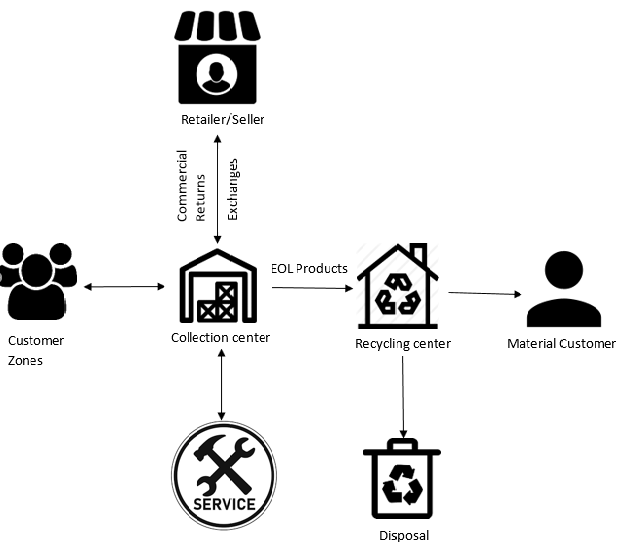
\includegraphics[width=0.75\textwidth]{FLowchat.png}
\caption{Reverse logistics network}
\label{fig:RLnetwork}
\end{figure}

\paragraph{Scope of the decision problem.} We emphasize at the outset that the problem studied here is a \emph{network planning (flow-allocation) problem} rather than a network \emph{design} problem. The locations and numbers of all facilities are fixed and known: a 3PL provider typically does not own the retailing, service, recycling, or disposal facilities, but operates collection centers and transportation services on behalf of its clients. Consequently, no facility-opening or location variables appear in the model. The decisions available to the 3PL are
\begin{enumerate}
    \item the \emph{tactical} assignment of customer zones to the collection centers it manages, which is fixed in the service contract before actual return volumes are observed, and 
    \item the \emph{operational} flow quantities routed between the facilities of the network once returns materialize.
\end{enumerate}
This scope reflects the contractual reality of third-party reverse logistics and distinguishes our formulation from facility-location-based reverse network design models such as \citet{zeballos2018integrating, Yavari2019}.

The network consists of customer zones, collection centers, service centers, retailing centers, recycling centers, and disposal locations. The process starts when customers place return orders for commercial returns, end-of-life (EOL) returns, or repairs. The products are collected from the customer zones by the 3PL and transported to a 3PL-managed collection center, where they are inspected and sorted. Commercial returns and exchanges are shipped to the retailing centers. Products requiring repair are transported to the service centers and, after repair, are \emph{shipped back by the 3PL from the service centers to the customer zones}; this return leg is modelled explicitly through its own flow variables and transportation cost. EOL returns are sent to the recycling centers, where raw materials are recovered; the residual fraction is transported to disposal locations as e-waste. All transportation, inspection, sorting, and storage activities, as well as e-waste disposal, are carried out by the 3PL.

\paragraph{Uncertainty and decision sequence.} Uncertainty in the collection of returned products is pronounced in third-party reverse logistics because the 3PL handles returns for multiple clients with different return policies, product types, and consumer behavior. The quantity of returns placed at each customer zone, the effective capacity of the collection centers, the inspection/sorting and storage costs, and the turnaround times of repaired products are not known with certainty at the moment the 3PL commits to its collection plan. We therefore formulate the problem as a \emph{two-stage stochastic program with recourse}. In the first stage, before the uncertain parameters are realized, the 3PL fixes the assignment of customer zones to collection centers. In the second stage, after observing a realization of the uncertain parameters, the 3PL decides the recourse flow quantities throughout the network, together with the amount of returns that remain uncollected. Uncertainty is represented by a finite set of scenarios $\Omega$ with occurrence probabilities $p_{\omega}$, $\sum\limits_{\omega \in \Omega} p_{\omega} = 1$, generated by Monte Carlo sampling from the specified distributions of the uncertain parameters (a sample average approximation of the underlying stochastic program). The quality of the resulting solutions is assessed on independently generated out-of-sample scenarios in Section 5.
\subsection{Mathematical Programming Model}\label{mathematical-programming-model}
In this subsection, we present the two-stage stochastic flow-allocation model that determines the assignment of customer zones to collection centers and the scenario-dependent quantities of products transported across the network, so as to jointly minimize the expected operating cost of the 3PL and the expected service-level penalties. The following assumptions are made. The sets, parameters, and decision variables are summarized in Table-\protect\hyperlink{t1}{2}, Table \protect\hyperlink{t2}{3}, Table-\ref{tab:uparam} and Table-\ref{tab:Decision}.

\subsubsection*{Assumptions}\label{assumptions}
\begin{enumerate}
\def\labelenumi{\arabic{enumi}.}
\item
  The model is single-period and considers a single (aggregate) product family. Product units are treated as a divisible volume at the planning level; the managerial implications of these simplifications and possible multi-period, multi-product extensions are discussed in Section 6.
\item
  Locations and numbers of customer zones, collection centers, retailing centers, service centers, recycling centers, and disposal locations are fixed and known. No facility-opening decisions are made (flow-allocation scope, see above).
\item
  Collection centers are managed by the 3PL and their capacities are restricted and uncertain. The capacities of the remaining facilities are assumed to be non-binding within the planning horizon; this is stated explicitly as a model limitation.
\item
  The 3PL carries out all transportation activities between the facilities, including the return of repaired products from service centers to customer zones.
\item
  Each customer zone is served by exactly one collection center (single sourcing), fixed contractually before return quantities are observed.
\item
  Operations and financials of the secondary market and material customers are not known to the 3PL and are excluded. Costs of the value-adding activities performed at service, recycling, and recovery centers are borne by the respective facility owners, not by the 3PL, and are therefore outside the objective function; contractual transfer prices are beyond the scope of this study.
\item
  The sorting fractions $\beta_{K}$, $\beta_{S}$ and $\beta_{R}$ are parameters of the model and not decisions. They describe the condition of the returned products, which inspection at the collection center reveals and the 3PL cannot choose. The 3PL therefore decides how much to collect and where each stream is sent, but not how the collected volume divides among the retailing, repair and recycling channels. The fractions are deterministic, identical across collection centers and scenarios, and conserve flow: $\beta_{K}+\beta_{S}+\beta_{R} = 1$.
\item
  The uncertain parameters are the return quantities $R_i^{\omega}$, the collection-center capacities $\widetilde{Ca}_j^{\omega}$, the inspection/sorting costs $\widetilde{C}_j^{\omega}$, the storage costs $\widetilde{W}_j^{\omega}$, and the unit turnaround times $t_{si}^{\omega}$; all are scenario-dependent.
\end{enumerate}

\hypertarget{t1}{}
\begin{table}[!htb]
\footnotesize
\renewcommand{\arraystretch}{1.25}
\renewcommand{\arraystretch}{1.25}
\caption{Indices and sets}
\label{t1}
%\fontsize{12.00pt}{12.00pt}\selectfont
\begin{tabular}{p{2cm}p{6cm}}
\toprule
Notions & Descriptions\\
\midrule
$i \in I$ & Set of customer zones \\
$j \in J$ & Set of collection centers \\
$k \in K$ & Set of retailing centers \\
$s \in S$ & Set of service centers \\
$r \in R$ & Set of recycling centers \\
$x \in X$ & Set of disposal locations \\
$\omega \in \Omega$ & Set of scenarios \\
\bottomrule
\end{tabular}
\end{table}
\hypertarget{t2}{}
\begin{table}[!htb]
\footnotesize
\renewcommand{\arraystretch}{1.25}
\caption{Deterministic parameters}
\label{t2}
%\fontsize{12.00pt}{12.00pt}\selectfont
\begin{tabular}{p{2cm}p{13cm}}
\toprule
Notions & Descriptions\\
\midrule
$T_{no}$ & Transportation cost per unit product from $n \to o$, where\\
& $(n,o)\in\{(i,j),(j,k),(j,s),(s,i),(j,r),(r,x)\}$. \\
$d_x$ & Disposal cost per unit product at disposal location $x$. \\
$\phi_1$ & Penalty per unit of returned product not collected from the customer zones. \\
$\phi_2$ & Penalty per unit-period of late delivery of repaired products. \\
$\tau_i$ & Scheduled (contractual) delivery time at customer zone $i$. \\
$\beta_{K}$ & Fraction of collected returns classified as commercial returns (to retailing centers). \\
$\beta_{S}$ & Fraction of collected returns classified as repairs (to service centers). \\
$\beta_{R}$ & Fraction of collected returns classified as EOL returns (to recycling centers). \\
$\alpha$ & Fraction of recycled volume generated as e-waste. \\
$p_{\omega}$ & Occurrence probability of scenario $\omega$, $\sum\limits_{\omega} p_{\omega}=1$. \\
\bottomrule
\end{tabular}
\end{table}
\hypertarget{t2b}{}
\begin{table}[!htb]
\footnotesize
\renewcommand{\arraystretch}{1.25}
\caption{Scenario-dependent (uncertain) parameters}
\label{tab:uparam}
%\fontsize{12.00pt}{12.00pt}\selectfont
\begin{tabular}{p{1.5cm}p{13.5cm}}
\toprule
Notions & Descriptions\\
\midrule
$R_i^{\omega}$ & Number of return orders placed at customer zone $i$ under scenario $\omega$. \\
$\widetilde{C}_j^{\omega}$ & Inspection and sorting cost per unit at collection center $j$ under scenario $\omega$. \\
$\widetilde{W}_j^{\omega}$ & Storage/warehousing cost per unit at collection center $j$ under scenario $\omega$. \\
$\widetilde{Ca}_j^{\omega}$ & Capacity of collection center $j$ under scenario $\omega$. \\
$t_{si}^{\omega}$ & Unit turnaround time of the repair channel serving zone $i$ via service center $s$ under scenario $\omega$ (collection, repair, and redelivery). \\
$\delta_{si}^{\omega}$ & Unit lateness of the repair channel, $\delta_{si}^{\omega}=\max(t_{si}^{\omega}-\tau_i,\,0)$, computed per scenario. \\
\bottomrule
\end{tabular}
\end{table}

\hypertarget{tab:Decision}{}
\begin{table}[!htb]
\footnotesize
\caption{Decision variables}
\label{tab:Decision}
\renewcommand{\arraystretch}{1.25}
%\fontsize{12.00pt}{12.00pt}\selectfont
\begin{tabular}{p{1.5cm}p{13.5cm}}
\toprule
Notions & Descriptions\\
\midrule
\multicolumn{2}{l}{\emph{First stage}} \\
\midrule
$y_{ij}$ & Binary; equals 1 if customer zone $i$ is assigned to collection center $j$, 0 otherwise. \\
\midrule
\multicolumn{2}{l}{\emph{Second stage (recourse, per scenario $\omega$)}} \\
\midrule
$Q_{ij}^{\omega}$ & Quantity collected from customer zone $i$ and shipped to collection center $j$. \\
$Q_{jk}^{\omega}$ & Quantity of commercial returns shipped from collection center $j$ to retailing center $k$. \\
$Q_{js}^{\omega}$ & Quantity of repairable products shipped from collection center $j$ to service center $s$. \\
$Q_{si}^{\omega}$ & Quantity of repaired products shipped back from service center $s$ to customer zone $i$. \\
$Q_{jr}^{\omega}$ & Quantity of EOL returns shipped from collection center $j$ to recycling center $r$. \\
$Q_{rx}^{\omega}$ & Quantity of e-waste shipped from recycling center $r$ to disposal location $x$. \\
$U_i^{\omega}$ & Quantity of returns at customer zone $i$ left uncollected. \\
\bottomrule
\end{tabular}
\end{table}
\protect\hypertarget{tab:Decision}{}{}


\subsection{Objective Functions and Constraints}
\label{objective-functions-and-constraints}
The first objective minimizes the total expected cost incurred by the 3PL throughout the reverse logistics process: transportation across all echelons of the network (including the return leg of repaired products from the service centers to the customer zones), inspection and sorting at the collection centers, storage, and disposal.
\begin{align}
    Minimize \hspace{10pt} Z_1 & = \sum_{\omega \in \Omega} p_{\omega} \Bigg[ \sum_i\sum_j \big(T_{ij}+\widetilde{C}_j^{\omega}+\widetilde{W}_j^{\omega}\big) Q_{ij}^{\omega} + \sum_j\sum_k T_{jk}Q_{jk}^{\omega} + \sum_j\sum_s T_{js}Q_{js}^{\omega} &&\notag\\
    & \hspace{45pt} + \sum_s\sum_i T_{si}Q_{si}^{\omega} + \sum_j\sum_r T_{jr}Q_{jr}^{\omega} + \sum_r\sum_x \big(T_{rx}+d_x\big) Q_{rx}^{\omega} \Bigg] \label{eqn-1}\tag{3.2.1}
\end{align}

Note that the transportation of repaired products back to the customer zones is now represented by the explicit flow variables $Q_{si}^{\omega}$ with their own unit cost $T_{si}$; this replaces the factor of two that multiplied the $j \rightarrow s$ transportation term in an earlier version of the model, which had implicitly (and opaquely) charged the return trip at the forward-trip rate.

The second objective minimizes the expected service-level penalties: the penalty for returned products left uncollected at the customer zones and the penalty for late redelivery of repaired products. Both terms are monetized through the contractual penalty rates $\phi_1$ (per uncollected unit) and $\phi_2$ (per unit-period of lateness), so the
two components of $Z_2$ are expressed in the same monetary unit and are directly commensurable.

\begin{flalign}
    Minimize \hspace{10pt} Z_2 & = \sum_{\omega \in \Omega} p_{\omega} \Bigg[ \phi_1 \sum_i U_i^{\omega} + \phi_2 \sum_s\sum_i \delta_{si}^{\omega} Q_{si}^{\omega} \Bigg] \label{eqn-2}\tag{3.2.2}
\end{flalign}
subject to
\begin{align}
    & \sum_{j} y_{ij} = 1 \hspace{215pt} \forall i \label{c1}\tag{3.2.3}\\
    & \sum_{j} Q_{ij}^{\omega} + U_i^{\omega} = R_i^{\omega} \hspace{170pt} \forall i, \omega \label{c2}\tag{3.2.4}\\
    & Q_{ij}^{\omega} \leq R_i^{\omega}\, y_{ij} \hspace{190pt} \forall i, j, \omega \label{c3}\tag{3.2.5}\\
    & \sum_{i} Q_{ij}^{\omega} \leq \widetilde{Ca}_j^{\omega} \hspace{190pt} \forall j, \omega \label{c4}\tag{3.2.6}\\
    & \sum_{k} Q_{jk}^{\omega} = \beta_{K} \sum_i Q_{ij}^{\omega} \hspace{160pt} \forall j, \omega \label{c5}\tag{3.2.7}\\
    & \sum_{s} Q_{js}^{\omega} = \beta_{S} \sum_i Q_{ij}^{\omega} \hspace{160pt} \forall j, \omega \label{c6}\tag{3.2.8}\\
    & \sum_{r} Q_{jr}^{\omega} = \beta_{R} \sum_i Q_{ij}^{\omega} \hspace{160pt} \forall j, \omega \label{c7}\tag{3.2.9}\\
    & \sum_{i} Q_{si}^{\omega} = \sum_{j} Q_{js}^{\omega} \hspace{175pt} \forall s, \omega \label{c8}\tag{3.2.10}\\
    & \sum_{s} Q_{si}^{\omega} = \beta_{S} \big(R_i^{\omega} - U_i^{\omega}\big) \hspace{140pt} \forall i, \omega \label{c9}\tag{3.2.11}\\
    & \sum_{x} Q_{rx}^{\omega} = \alpha \sum_j Q_{jr}^{\omega} \hspace{170pt} \forall r, \omega \label{c10}\tag{3.2.12}\\
    & y_{ij} \in \{0,1\}; \hspace{6pt} Q_{ij}^{\omega}, Q_{jk}^{\omega}, Q_{js}^{\omega}, Q_{si}^{\omega}, Q_{jr}^{\omega}, Q_{rx}^{\omega}, U_i^{\omega} \geq 0 \hspace{22pt} \forall i,j,k,s,r,x,\omega \label{c11}\tag{3.2.13}
\end{align}

Constraint~\ref{c1} is the first-stage single-sourcing condition: each customer zone is assigned to exactly one collection center before the uncertainty is realized. Constraint~\ref{c2} is the collection balance at each customer zone: under every scenario, the realized returns are either collected or accounted for as uncollected volume $U_i^{\omega}$, which is penalized in $Z_2$. Constraint~\ref{c3} links the two stages: products can flow from zone $i$ to collection center $j$ only if the assignment $y_{ij}$ was made in the first stage, and never in excess of the realized returns. Constraint~\ref{c4} enforces the (uncertain) capacity of each collection center under every scenario. Constraints~\ref{c5}--\ref{c7} are the flow-balance (sorting) constraints at each collection center $j$: the inbound collected volume is split into commercial returns, repairs, and EOL returns according to the sorting fractions. Because $\beta_{K}+\beta_{S}+\beta_{R}=1$ (Assumption 7), these three constraints jointly guarantee conservation of flow at the collection centers: every unit that enters a collection center leaves it through exactly one of the three downstream channels. Constraint~\ref{c8} is the flow balance at each service center: all repaired products are shipped back to the customer zones. Constraint~\ref{c9} ensures that each customer zone receives back the repaired share of its own collected returns, so that redelivery volumes are consistent with collection volumes at the zone level. Constraint-\ref{c10} balances the recycling centers: the fraction $\alpha$ of the recycled volume is generated as e-waste and must be shipped to the disposal locations. Constraint~\ref{c11} declares the variable domains explicitly: the first-stage assignment variables are binary, whereas all flow and shortage variables are continuous and nonnegative, product volume being treated as divisible at the planning level (Assumption 1). The model is therefore a \emph{bi-objective two-stage stochastic mixed-integer linear program (MILP)}.

\paragraph{Treatment of the lateness term.} The unit lateness $\delta_{si}^{\omega} = \max(t_{si}^{\omega}-\tau_i,\,0)$ is a \emph{parameter} computed for each scenario from the realized turnaround time $t_{si}^{\omega}$ and the contractual delivery time $\tau_i$; it is not a decision variable, so no nonlinearity enters the model and $Z_2$ is linear in the decision variables. Should turnaround times be made endogenous in future extensions (e.g., workload-dependent repair times), the max-operator can be linearized in the standard way by introducing auxiliary variables $\delta_{si}^{\omega} \geq t_{si}^{\omega} - \tau_i$, $\delta_{si}^{\omega} \geq 0$, which is exact whenever $\delta_{si}^{\omega}$ is penalized in a minimization objective.

\subsection{Model Properties and Computational Complexity}
\label{model-properties-and-computational-complexity}
The deterministic single-scenario restriction of the model already contains the single-source capacitated assignment structure induced by constraints~\ref{c1}, \ref{c3} and \ref{c4}, which includes the generalized assignment problem as a special case and is therefore NP-hard \citep{Garey, wolsey1998integer}. Three features compound the computational burden. First, the problem is bi-objective: cost minimization and service-level improvement conflict, so the solution concept is the Pareto-optimal set rather than a single optimum. Second, the two-stage stochastic structure replicates all recourse variables and constraints for every scenario $\omega \in \Omega$, so the model size grows linearly in $|\Omega|$ and realistic scenario counts yield large-scale MILPs. Third, the network spans multiple echelons with interdependent flow balances. These properties make the worst case hard. They do not show that the instances studied here are beyond a general-purpose solver, and Section~\ref{validation-against-exact-solutions} reports how far the $\epsilon$-constraint method gets on them under a stated time budget. The approximate method of Section~4 is motivated by run time, not by a claim that exact solution is out of reach at benchmark size.

\begin{example}
To fix ideas, consider a network with two customer zones, one collection center, and one facility of each remaining type, under a single scenario $\omega$ with $R_1^{\omega}=100$, $R_2^{\omega}=80$, and $\widetilde{Ca}_1^{\omega}=150$, with sorting fractions $\beta_K=0.5$, $\beta_S=0.3$, $\beta_R=0.2$ and e-waste fraction
$\alpha=0.4$. Both zones are assigned to the single collection center ($y_{11}=y_{21}=1$). Since the realized returns (180) exceed the realized capacity (150), the recourse decision collects $Q_{11}^{\omega}=100$ and $Q_{21}^{\omega}=50$, leaving $U_2^{\omega}=30$ units uncollected and penalized at rate $\phi_1$ in $Z_2$. The collected volume of 150 is sorted into
$0.5 \times 150 = 75$ units to the retailing center,
$0.3 \times 150 = 45$ units to the service center, and
$0.2 \times 150 = 30$ units to the recycling center (constraints
\ref{c5}--\ref{c7}). The 45 repaired units are redelivered to the zones in proportion to their collected repair shares (constraint~\ref{c9}):
$Q_{s1}^{\omega}$ delivers $0.3 \times 100 = 30$ units to zone 1 and
$0.3 \times 50 = 15$ units to zone 2. If the realized turnaround time
for zone 1 is $t_{s1}^{\omega}=5$ against a contractual $\tau_1=4$,
the lateness parameter is $\delta_{s1}^{\omega}=1$ and the
corresponding penalty in $Z_2$ is $\phi_2 \times 1 \times 30$.
Finally, $0.4 \times 30 = 12$ units of e-waste flow to the disposal
location (constraint~\ref{c10}), incurring
transportation and disposal costs in $Z_1$.
\end{example}
The resulting bi-objective formulation balances the 3PL's expected operating cost against its expected contractual service performance under return, capacity, cost, and turnaround-time uncertainty, while keeping every modelling element within the decision authority of a third-party provider: assignment of zones to collection centers, recourse flow allocation, and explicit accounting of uncollected and late volumes. The model is stated with full recourse: the flows $Q^{\omega}$ and the uncollected volumes $U_i^{\omega}$ in Table~\ref{tab:Decision} may take any feasible value in each scenario. The solution method of Section~4 does not search this whole space. It works with a restricted class of recourse policies, and the difference between the two is set out in Section~\ref{sec:representation}.
\section{Solution methodology}
The model formulated in Section~3 is a bi-objective two-stage stochastic mixed-integer linear program whose deterministic counterpart already contains an NP-hard single-source capacitated assignment problem. Furthermore, the problem size increases linearly with the number of scenarios considered. Worst-case complexity does not settle whether a given instance can be solved in practice. With an open-source solver and 300 seconds per subproblem, the $\epsilon$-constraint method applied to the scenario-expanded MILP proves optimality at every grid point up to instance~5 and at all but one to three of the 21 points up to instance~12. On the largest instance it still returns incumbents with certified gaps of about 4\% at most in a little under two hours (Section~\ref{validation-against-exact-solutions}). Exact solution is therefore available as a reference on this benchmark, and we use it as one. What an evolutionary method offers here is run time: seconds per run where the exact grid takes from under a minute to about two hours. This holds from instance~3 onwards. On instances 1 and 2 the exact method is as fast as the evolutionary method or faster.

To obtain approximate fronts quickly, we propose an \emph{Enhanced NSGA-II} (E-NSGA-II), an improved variant of the Non-Dominated Sorting Genetic Algorithm II developed by \citet{Kdeb2002}. The proposed algorithm incorporates three problem-specific enhancements:
\begin{enumerate}
    \item A heuristic initialization procedure to generate high-quality initial solutions,
    \item A feasibility repair operator to ensure constraint satisfaction following genetic operations, and 
    \item An adaptive mutation strategy that dynamically balances exploration and exploitation throughout the evolutionary search.
\end{enumerate}
E-NSGA-II is compared against three multi-objective evolutionary algorithms, each representing a different optimization approach: MOEA/D-DE, which uses decomposition and differential evolution operators; SMS-EMOA, which selects solutions based on hypervolume contribution; and SPEA2, which is a Pareto-based method that uses an archive and density-based selection.
\iffalse
\subsection{Positioning of the methodological
contribution}\label{positioning-of-the-methodological-contribution}
Before describing the algorithms, we explicitly state what is new in the solution methodology relative to the common practice in metaheuristic studies of reverse logistics networks (the structural novelty of the model itself—the 3PL decision scope, the two-stage assignment-plus-recourse structure, the explicit repair-return leg, and the penalty-based service objective—is positioned against the literature in \textcolor{red}{Section 2}). Algorithmically, this study contributes:

\begin{enumerate}
\def\labelenumi{\arabic{enumi}.}
\item
  A problem-specific two-part encoding that combines integer assignment genes (the first-stage variables $y_{ij}$) with continuous collection-intensity genes $\rho_i$, so that the chromosome spans both stages of the stochastic program and the intensity genes generate the cost--service Pareto trade-off directly;
\item
  A heuristic initialization scheme that seeds the population with capacity-aware greedy assignments and economically graded collection intensities, giving the search immediate access to structurally strong first-stage plans;
\item
  A feasibility repair operator based on proportional capacity scaling, which maps every chromosome to flows satisfying all constraints-\eqref{c1}--\eqref{c11}
  by construction, so the search never leaves the feasible region and no penalty functions are required;
\item
  An adaptive mutation mechanism that reacts to diversity loss and hypervolume stagnation, directly countering the Pareto-front crowding observed in preliminary experiments and flagged as an open issue in the previous version of this work;
\item
  Scenario-based fitness evaluation with common random numbers inside the evolutionary loop (sample-average approximation), with out-of-sample validation, complemented by a decision-closure layer (knee-point analysis and TOPSIS ranking) that converts the final front into an implementable operating plan.
\end{enumerate}
\begin{table}[htbp]
\centering
\caption{Algorithmic positioning of this study}
\label{tab:AlgPositioning}
\renewcommand{\arraystretch}{1.2}
\fontsize{10.00pt}{10.00pt}\selectfont
\begin{tabular}{p{2.1cm}p{6.0cm}p{6.2cm}}
\toprule
\textbf{Design element} &
\textbf{Common practice in RL metaheuristic studies} &
\textbf{This study (E-NSGA-II)} \\
\midrule
Encoding &
Flow quantities or priorities, single-stage representation &
Two-part encoding: first-stage customer assignments and collection intensities \\
\midrule
Initialization &
Uniform random initialization &
Capacity-aware greedy initialization with graded collection intensities (30\%) and random initialization (70\%) \\
\midrule
Feasibility handling &
Penalty functions or discard-and-resample strategies &
Proportional capacity repair ensuring feasible solutions after every genetic operation \\
\midrule
Diversity management &
Fixed mutation probability &
Adaptive mutation guided by population diversity and stagnation indicators \\
\midrule
Uncertainty in evaluation &
Deterministic evaluation or single sampled realization &
Sample-average evaluation over common in-sample scenarios with additional out-of-sample validation \\
\midrule
Benchmark suite &
Comparison against algorithms from the same family &
Comparison with decomposition-based (MOEA/D-DE), indicator-based (SMS-EMOA), and archive-based (SPEA2) algorithms \\
\midrule
Algorithm assessment &
CPU time and number of non-dominated solutions &
Hypervolume (HV), IGD$^{+}$, spread metric, and statistical tests under equal evaluation budgets \\
\midrule
Post-optimization decision &
Pareto front reported directly &
Knee-point identification combined with TOPSIS and weight sensitivity analysis \\
\bottomrule
\end{tabular}
\end{table}\fi
\subsection{Solution representation and decoding}\label{sec:representation}
A candidate solution must specify the first-stage assignment of customer
zones to collection centers and imply, for every scenario, a feasible
set of recourse flows. In the model of Section~3 these flows are chosen freely in each scenario. The algorithm does not encode them directly. It encodes a collection rule that is fixed before the uncertainty is realized, and the decoder generates the scenario flows from that rule. The search is therefore carried out over a restricted class of recourse policies. The restriction and its consequences are stated at the end of this subsection. We use a two-part chromosome of length $2|I|$:

\begin{enumerate}
\def\labelenumi{\arabic{enumi}.}
\item
  \textbf{Assignment part} $a = (a_1, \ldots, a_{|I|})$, where $a_i \in \{1, \ldots, |J|\}$ encodes the collection center to which customer zone $i$ is assigned; this is an integer encoding of the binary first-stage variables ($y_{ij} = 1 \Leftrightarrow a_i = j$) that satisfies the single-sourcing constraint-\eqref{c1} by construction.
\item
  \textbf{Collection-intensity part}
  $\rho = (\rho_1, \ldots, \rho_{|I|})$, where $\rho_i \in [0,1]$ is the fraction of the realized returns of zone $i$ that the 3PL attempts to collect. The intensity genes carry no scenario index: $\rho$ is chosen together with $a$ and the same value $\rho_i$ is applied in every scenario. The intensity genes let the population trade collection cost in $Z_1$ against the uncollected-returns penalty in $Z_2$, which is the tension that generates the Pareto
  front.
\end{enumerate}

\textbf{Decoding.} Given a chromosome $(a, \rho)$ and a scenario $\omega$, the recourse flows are constructed as follows.

\begin{enumerate}
\def\labelenumi{\arabic{enumi}.}
\item
  \emph{Attempted collection}: zone $i$ tenders $\rho_i R_i^{\omega}$ units to collection center $a_i$.
\item
  \emph{Feasibility repair} (described below): tendered volumes are
  scaled so that the capacity constraint-\eqref{c4} holds at every collection center; residual quantities join $U_i^{\omega}$.
\item
  \emph{Sorting}: the inbound volume at each collection center is split into the three downstream channels by the fractions $\beta_K, \beta_S, \beta_R$ (constraints-\eqref{c5}--\eqref{c7}).
\item
  \emph{Downstream allocation}: commercial returns are routed from each collection center to its cheapest retailing center ($\argmin_k T_{jk}$), EOL returns to the cheapest recycling center, and e-waste from each recycling center to the cheapest disposal location; since these facilities are uncapacitated (Assumption 3), the
  greedy choice is optimal for any fixed collection plan, these flows entering only $Z_1$. Repairable volumes are routed to the service center minimizing the round-trip transportation cost $T_{js} + T_{si}$ of the originating zone, and the repaired units return to their zones according to constraint-\eqref{c9}. This last choice is made on cost alone and does not look at the scenario lateness $\delta_{si}^{\omega}$.
\item
  \emph{Evaluation}: the scenario costs and penalties are accumulated and averaged over the scenario set to yield the sample-average objective vector ($Z_1, Z_2$).
\end{enumerate}

All individuals of all algorithms are evaluated on the \emph{same}
in-sample scenario set (common random numbers), which removes evaluation
noise from the comparison between algorithms; solution quality is
subsequently re-assessed on an independent out-of-sample scenario set in
Section 5.

\paragraph{Relation to the two-stage model.} The decoder is a recourse policy in the sense of a decision rule \citep{bental2004adjustable, kuhn2011primal}: it maps the pair $(a,\rho)$ and the realization $\omega$ to a complete set of flows. For every chromosome and every scenario these flows satisfy constraints-\eqref{c2}--\eqref{c11}, so each decoded solution is feasible for the two-stage model and its objective vector is attainable. The policy is nevertheless a restriction of the recourse declared in Table~\ref{tab:Decision}, in three respects.
\begin{enumerate}
\item The collected quantity is
\begin{equation}
Q_{i a_i}^{\omega} = \rho_i R_i^{\omega}\,\min\!\left\{1,\, \widetilde{Ca}_{a_i}^{\omega} \big/ V_{a_i}^{\omega}\right\},
\qquad V_j^{\omega} = \sum_{i:\, a_i = j} \rho_i R_i^{\omega},
\label{eq:policy}\tag{4.1.1}
\end{equation}
so it responds to the scenario only through the realized returns and the capacity of the assigned center. The fraction $\rho_i$ is a here-and-now quantity. It cannot be raised in scenarios where capacity is slack or the handling costs $\widetilde{C}_j^{\omega}$ and $\widetilde{W}_j^{\omega}$ are low, and it cannot be lowered in the opposite case, whereas the model allows both.
\item When capacity binds, the shortfall is shared in proportion to the tendered volumes of the zones assigned to the center. The full recourse would instead give priority to the zones whose cost and penalty terms are most favourable in that scenario. In the example of Section~\ref{model-properties-and-computational-complexity} the recourse collects 100 and 50 units from the two zones, whereas the rule with $\rho_1=\rho_2=1$ collects 83.3 and 66.7.
\item The service center of each zone is selected by round-trip cost, which is the best choice for $Z_1$ but ignores the lateness term of $Z_2$.
\end{enumerate}
E-NSGA-II and the three benchmark algorithms of Section~\ref{sec:benchmarks} share this decoder. All four therefore search over the pairs $(y,\rho)$ and not over the recourse space of the model, and the fronts reported in Section~5 are fronts of this policy-restricted problem. Because the restricted feasible set is contained in the feasible set of the two-stage model, these fronts approximate the two-stage Pareto front from the inside: every reported point can be achieved, but points of the two-stage front may dominate it. The method should accordingly be read as an approximate solution method for the two-stage model and not as an exact treatment of its recourse. Section~\ref{validation-against-exact-solutions} measures the loss against $\epsilon$-constraint reference fronts. The comparison among the four algorithms is not affected by the restriction, since all of them search the same policy class.

The rule has two practical properties that we use later. A selected plan $(a,\rho)$ can be applied to a realization that was not in the sample without solving any optimization problem, which is how the out-of-sample evaluation of Section~\ref{out-of-sample-evaluation} is carried out, and one evaluation of a chromosome costs $O(|I||\Omega|)$ arithmetic operations. The restriction is not, however, forced by the problem. For a fixed assignment, a fixed scenario and a weight $\lambda\in[0,1]$ placed on $Z_1$ against $Z_2$, the recourse problem is a linear program. Since the downstream facilities are uncapacitated (Assumption 3), it separates by collection center into a continuous knapsack problem: each unit collected from zone $i$ has a scenario-specific weighted net value, obtained from its collection and downstream costs, the avoided penalty $\phi_1$ and the lateness of its best service center, and the capacity of the center is filled in decreasing order of this value. Solving this problem inside the decoder, with $\lambda$ carried as a gene in place of $\rho$, lets the collected fraction depend on the scenario and removes the first two restrictions listed above. We have implemented this variant with the service center still chosen by cost, and tested it on instances 1--3 only. Section~\ref{validation-against-exact-solutions} reports the result: it stays at the level of the reference on every instance tested, where the collection rule recovers between 28\% and 89\% of the reference hypervolume. %All other experiments in Section~5 use the collection rule, and re-running them with the recourse decoder is listed in Section~7 as the first extension of this work.
\subsection{The Proposed E-NSGA-II}
E-NSGA-II retains the elitist framework of NSGA-II, including non-dominated sorting, crowding-distance diversity preservation, binary tournament selection, and $\mu + \lambda$ environmental selection. It augments this framework with the three components described below. The complete procedure is illustrated in Figure-\ref{fig:ensga2} and summarized in Algorithm-\ref{alg:ensga2}.
\subsubsection{{Heuristic Initialization}}
A fraction $\eta$ of the initial population (we use $\eta = 0.3$; sensitivity to $\eta$ is reported in Section 5) is constructed heuristically; the remainder is generated uniformly at random to protect diversity. Each heuristic individual is built in two steps.
\begin{itemize}
    \item \emph{Assignment genes}: customer zones are considered in decreasing
order of expected returns $\bar{R}_i$ and assigned greedily to the collection center with the lowest unit collection cost $T_{ij} + \bar{C}_j + \bar{W}_j$ among centers whose residual expected capacity can absorb the zone's expected volume; when no center has residual capacity, the cheapest center is chosen regardless (the repair operator restores feasibility scenario-wise). Randomized tie-breaking across the ordered candidate list produces distinct seeds.
\item \emph{Intensity genes}: since collecting one unit from zone $i$ costs approximately $T_{i a_i} + \bar{C}_{a_i} + \bar{W}_{a_i}$ plus downstream handling, whereas leaving it uncollected incurs $\phi_1$, the economic pressure to collect is summarized by the ratio of penalty to marginal cost. The seeds grade their intensities along this ratio: individuals intended for the cost-efficient end of the front receive $\rho_i$ proportional to the (normalized) penalty-to-cost ratio of zone $i$, while individuals intended for the service end receive $\rho_i$ close to 1. Spreading the seeds along this economic gradient covers the anticipated span of the Pareto front from the first generation onwards.
\end{itemize}
\subsubsection{Feasibility Repair Operator}
Crossover and mutation always produce syntactically valid chromosomes (assignment genes remain in $\{1,\ldots,|J|\}$ and intensity genes are truncated to $[0,1]$), but the implied collection plan may violate the scenario capacities. The repair operator restores feasibility inside the decoder: for each scenario $\omega$ and each collection center $j$ whose tendered volume $V_j^{\omega} = \sum\limits_{i: a_i = j} \rho_i R_i^{\omega}$ exceeds $\widetilde{Ca}_j^{\omega}$, all collected quantities of the zones assigned to $j$ are scaled by the factor $\widetilde{Ca}_j^{\omega} / V_j^{\omega}$, and the displaced volume is recorded as uncollected ($U_i^{\omega}$), where it is penalized in $Z_2$. Repair is therefore proportional (it preserves the relative collection policy expressed by the genes), scenario-exact (feasibility holds for every realization, not merely in expectation), and free of penalty-function calibration. Because repair acts within the decoding step, the genotype is left untouched and no repair-induced genetic drift occurs.
\subsubsection{Genetic Operators and Adaptive
Mutation}
The assignment part uses integer-coded single-point or two-point crossover (both are examined in the experimental design of Section 5) with a reassignment mutation that replaces $a_i$ by a center drawn uniformly at random; the intensity part shares the crossover cut points and uses a creep mutation that perturbs $\rho_i$ by a uniform step of half-width $\sigma$, truncated to $[0,1]$.

Preliminary experiments, together with feedback from the reviewers of an earlier version of this paper, identified the crowding of the Pareto front as a limitation of the standard configuration. E-NSGA-II therefore adapts its mutation pressure according to two run-time signals. Let $\Delta_t$ denote the normalized spread of the first front at generation $t$, computed as the average crowding distance of the non-boundary
members normalized by its running maximum, and let $s_t$ denote the number of consecutive generations without improvement in the in-sample hypervolume. The per-gene mutation probability and the creep half-width are then set as
\begin{equation}
   p_m(t) = p_{\min} + \left(p_{\max}-p_{\min}\right)\left(1-\Delta_t\right),
\qquad
\sigma(t) = \sigma_0 \left(1 - \tfrac{t}{T}\right)\left(1 + \mathds{1}\{s_t \geq g_s\}\right), \tag{4.2.3.1}
\end{equation}
where $T$ is the generation budget and $g_s$ a stagnation threshold. When the front is well spread ($\Delta_t \to 1$), mutation recedes to the exploitation level $p_{\min}$; when solutions cluster ($\Delta_t \to 0$) or the hypervolume stalls for $g_s$ generations,
mutation pressure and step width increase, re-injecting the variation needed to escape crowded configurations. This mechanism operationalizes the diversity-preservation remedy that the earlier version of the paper only identified as future work.
\begin{figure}[htbp]
\centering
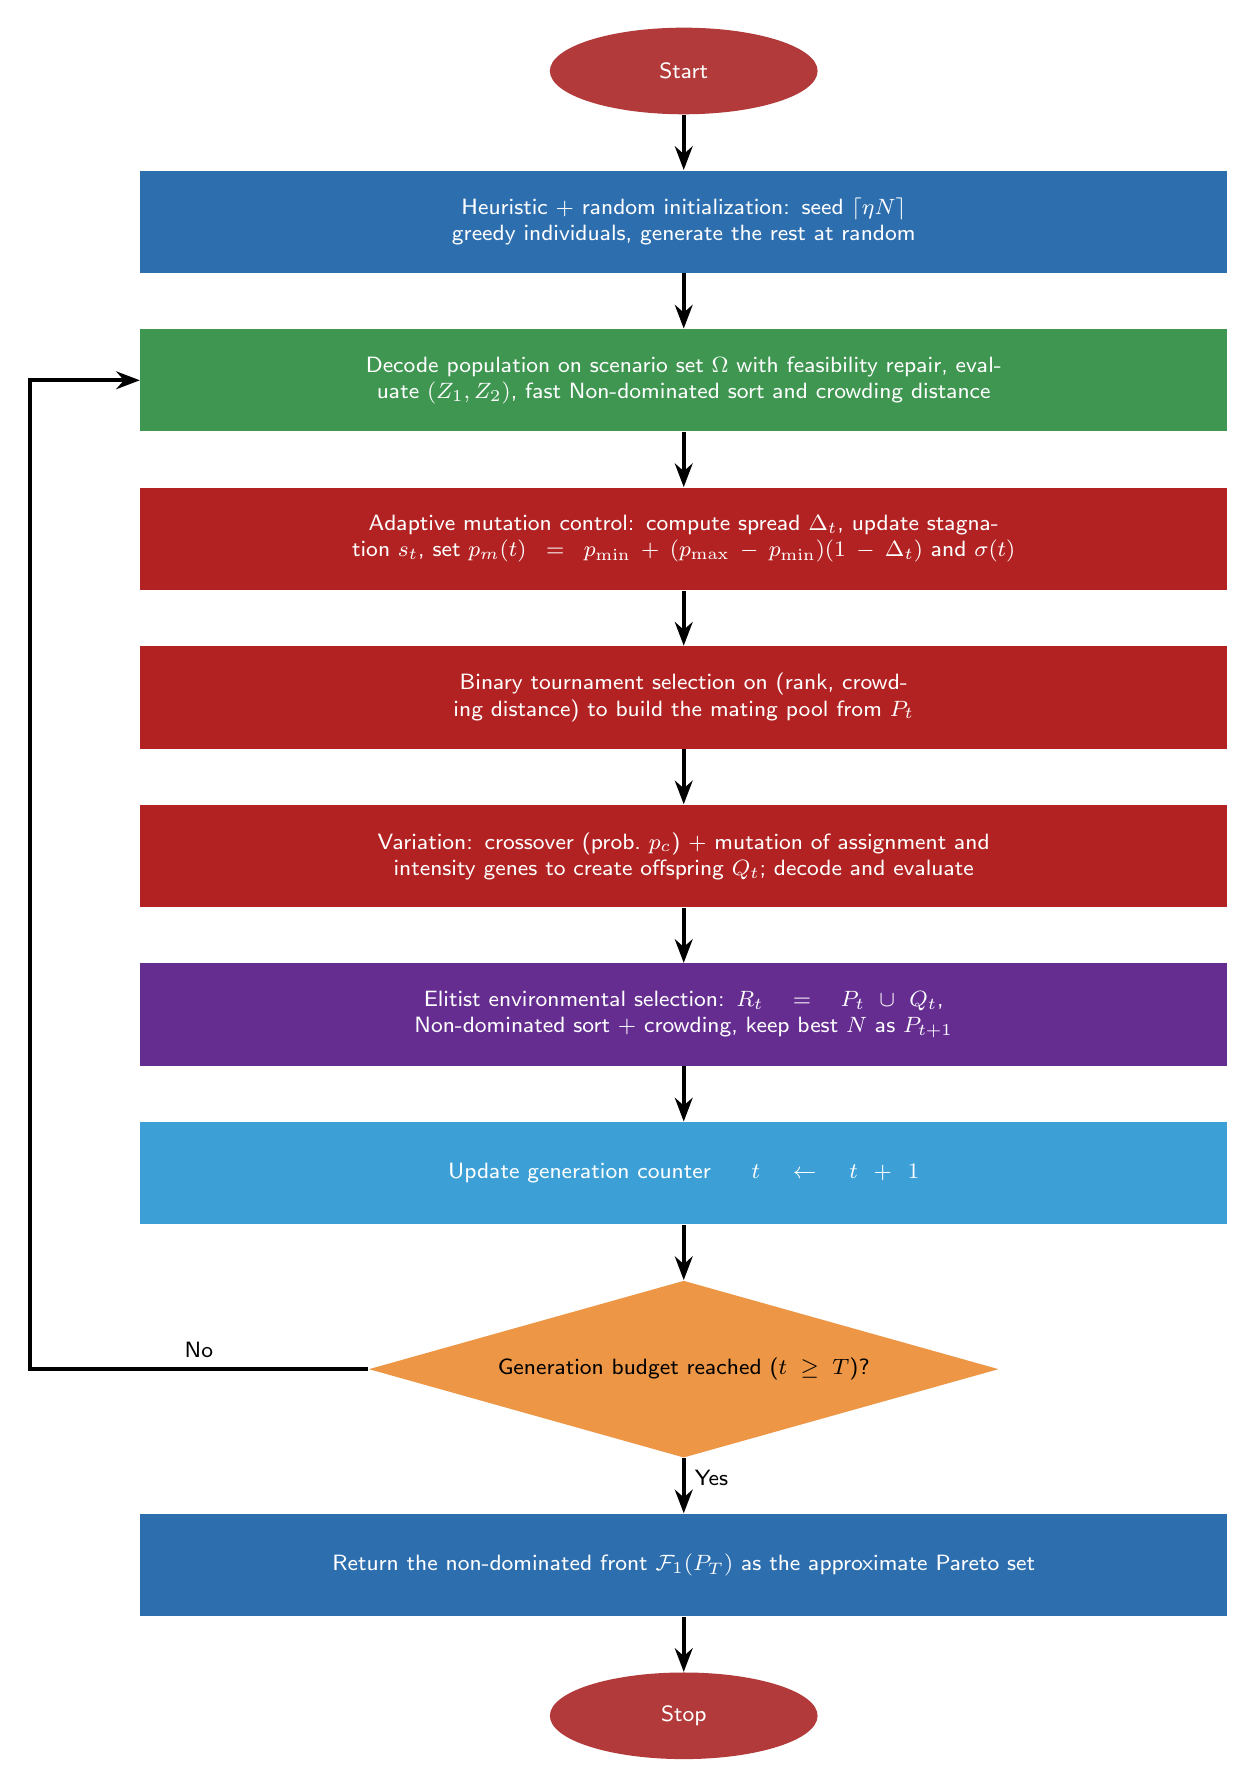
\begin{tikzpicture}[
  node distance = 7mm and 7mm,
  font = \sffamily\footnotesize,
  every node/.style = {align=center, text=white},
  box/.style   = {rectangle, minimum width=138mm, minimum height=13mm, inner sep=4pt, text width=108mm, align=center},
  term/.style  = {ellipse, minimum width=34mm, minimum height=11mm, fill=startred},
  dec/.style   = {diamond, aspect=3.2, inner sep=1pt, minimum width=80mm,
                   text width=60mm, fill=decorange, text=black},
  arr/.style   = {-{Stealth[length=3mm]}, line width=0.5mm, black}]
% ---- Nodes --------------------------------------------------------------

\node[term] (start) {Start};

\node[box, fill=initblue, below=of start] (init)
  {Heuristic + random initialization: seed $\lceil\eta N\rceil$ greedy
   individuals, generate the rest at random};

\node[box, fill=evalgreen, below=of init] (eval)
  {Decode population on scenario set $\Omega$ with feasibility repair,
   evaluate $(Z_1,Z_2)$, fast Non-dominated sort and crowding distance};

\node[box, fill=stepred, below=of eval] (adapt)
  {Adaptive mutation control: compute spread $\Delta_t$, update
   stagnation $s_t$, set $p_m(t)=p_{\min}+(p_{\max}-p_{\min})(1-\Delta_t)$
   and $\sigma(t)$};

\node[box, fill=stepred, below=of adapt] (select)
  {Binary tournament selection on (rank, crowding distance) to build the
   mating pool from $P_t$};

\node[box, fill=stepred, below=of select] (variation)
  {Variation: crossover (prob.\ $p_c$) + mutation of assignment and
   intensity genes to create offspring $Q_t$; decode and evaluate};

\node[box, fill=mutpurple, below=of variation] (env)
  {Elitist environmental selection: $R_t=P_t\cup Q_t$, Non-dominated
   sort + crowding, keep best $N$ as $P_{t+1}$};

\node[box, fill=updblue, below=of env] (update)
  {Update generation counter $\;t \leftarrow t+1$};

\node[dec, below=of update] (stop) {Generation budget reached ($t \geq T$)?};

\node[box, fill=initblue, below=of stop] (out)
  {Return the non-dominated front $\mathcal{F}_1(P_T)$ as the approximate
   Pareto set};

\node[term, below=of out] (end) {Stop};

% ---- Straight-through arrows -------------------------------------------
\draw[arr] (start)     -- (init);
\draw[arr] (init)      -- (eval);
\draw[arr] (eval)      -- (adapt);
\draw[arr] (adapt)     -- (select);
\draw[arr] (select)    -- (variation);
\draw[arr] (variation) -- (env);
\draw[arr] (env)       -- (update);
\draw[arr] (update)    -- (stop);
\draw[arr] (stop)      -- node[pos=0.35, right, text=black] {Yes} (out);
\draw[arr] (out)       -- (end);

% ---- "No" feedback loop back to the evaluation step --------------------
\coordinate (loop) at ($(eval.west)+(-14mm,0)$);
\draw[arr] (stop.west) -| node[pos=0.25, above, text=black] {No} (loop) -- (eval.west);

\end{tikzpicture}
\caption{Flowchart of the Enhanced NSGA-II (E-NSGA-II) for the
           bi-objective two-stage stochastic 3PL network planning model.}
  \label{fig:ensga2}
\end{figure}

\begin{algorithm}[!htb]
%\small
\DontPrintSemicolon
\SetKwFunction{HInit}{HeuristicInit}
\SetKwFunction{RInit}{RandomInit}
\SetKwFunction{Eval}{Evaluate}
\SetKwFunction{NDSort}{NDSort}
\SetKwFunction{Tour}{Tournament}
\SetKwFunction{Cross}{Crossover}
\SetKwFunction{Mut}{Mutate}
\SetKwFunction{HV}{Hypervolume}
\SetKwFunction{Spread}{Spread}
\caption{Enhanced NSGA-II (E-NSGA-II)}
\label{alg:ensga2}
\BlankLine
\KwInput{$N$, $\eta$, $p_c$, $p_{\min}$, $p_{\max}$, $\sigma_0$, $g_s$, $T$, $\Omega$, reference point $r$}
\KwOutput{Approximate Pareto front $\mathcal{F}_1(P_T)$}
$P_0 \leftarrow \HInit{\ensuremath{\lceil \eta N \rceil}} \,\cup\, \RInit{\ensuremath{N-\lceil \eta N \rceil}}$ \tcp*{greedy seeds + random fill}
\Eval{\ensuremath{P_0, \Omega}} \tcp*{decode $\rightarrow$ repair $\rightarrow$ $(Z_1,Z_2)$}
\NDSort{$P_0$}\;
$s \leftarrow 0$;\quad $h^{\ast} \leftarrow \HV{\ensuremath{\mathcal{F}_1(P_0), r}}$ \tcp*{best hypervolume so far}
\For{$t \leftarrow 0$ \KwTo $T-1$}{
  $\Delta_t \leftarrow \Spread{\ensuremath{\mathcal{F}_1(P_t)}}$;\quad
  $h_t \leftarrow \HV{\ensuremath{\mathcal{F}_1(P_t), r}}$\;
  \lIf{$h_t > h^{\ast}$}{$s \leftarrow 0$;\ $h^{\ast} \leftarrow h_t$}
  \lElse{$s \leftarrow s+1$}
  $p_m \leftarrow p_{\min} + (p_{\max}-p_{\min})(1-\Delta_t)$ \tcp*{more mutation when crowded}
  $\sigma \leftarrow \sigma_0 \left(1-t/T\right)\left(1+\mathds{1}\{s \geq g_s\}\right)$ \tcp*{decaying step; doubled on stall}
  $M_t \leftarrow \Tour{\ensuremath{P_t}}$ \tcp*{binary tournament on (rank, crowding)}
  $O_t \leftarrow \Cross{\ensuremath{M_t, p_c}}$\;
  $Q_t \leftarrow \Mut{\ensuremath{O_t, p_m, \sigma}}$ \tcp*{reassignment + creep on $[0,1]$}
  \Eval{\ensuremath{Q_t, \Omega}} \tcp*{common random numbers}
  $R_t \leftarrow P_t \cup Q_t$;\quad \NDSort{\ensuremath{R_t}}\;
  $P_{t+1} \leftarrow$ first $N$ of $R_t$ by (rank, crowding) \tcp*{elitist survival}
}
\KwRet{\ensuremath{\mathcal{F}_1(P_T)}}\;
\end{algorithm}

\subsection{Benchmark Algorithms and Rationale}\label{sec:benchmarks}
E-NSGA-II is compared against three algorithms chosen to represent the principal design philosophies of modern multi-objective evolutionary computation, all implemented with the same representation, decoder, repair operator, and function-evaluation budget to keep the comparison fair.

\textbf{MOEA/D-DE}\citep{li2009moeadde} decomposes the bi-objective problem into a set of scalarized subproblems (we use the Tchebycheff approach) optimized cooperatively through neighbourhood-based mating, and employs differential-evolution variation, which strengthens exploration of the continuous intensity genes relative to the original MOEA/D; integer assignment genes are varied with the reassignment operator after DE recombination, followed by repair. Decomposition typically accelerates convergence, but the distribution of the weight vectors governs the diversity of the resulting front.

\textbf{SMS-EMOA}\citep{beume2007smsemoa} is an indicator-based, steady-state algorithm that accepts a new individual only if it increases the dominated hypervolume of the population; in the bi-objective case the hypervolume contribution of each individual is computable in $O(N \log N)$ time per iteration, so the method remains computationally attractive while optimizing precisely the indicator by which fronts are commonly judged. Its inclusion places a \emph{newer, indicator-driven} selection paradigm in the comparison.

\textbf{SPEA2}\citep{zitzler2001spea2} maintains an external archive of non-dominated solutions and uses a $k$-nearest-neighbor density estimator in its fitness assignment, which tends to produce well-distributed fronts at the price of a higher computational cost per generation.

The composition of this suite also answers a natural question: why enhance NSGA-II rather than adopt one of its successors as the primary algorithm ? Reference-point- and reference-vector-based algorithms such as NSGA-III\citep{deb2014nsgaiii} and RVEA\citep{cheng2016rvea} were motivated by \emph{many}-objective problems (four or more objectives), where Pareto dominance loses selective pressure and crowding-based diversity maintenance degrades; for two objectives, dominance-based selection retains full pressure, the crowding distance is a reliable diversity measure, and empirical comparisons in the literature repeatedly find NSGA-II-class algorithms competitive with their successors in the bi-objective regime. We therefore invest the problem-specific knowledge where it demonstrably pays, namely initialization, feasibility repair, and diversity control. The benchmark suite, comprising decomposition-, indicator-, and archive-based selection mechanisms, then tests whether any competing paradigm outperforms the enhanced dominance-based design. The empirical comparison in Section 5 evaluates all four algorithms with standard multi-objective quality indicators (hypervolume, IGD+, spread) under identical budgets rather than by runtime alone, and includes an ablation study of the three enhancements.
\subsection{{From the Pareto front to an implementable decision}}
A Pareto front is a decision-support artifact, not a decision. To close
the loop for managerial implementation, we apply a two-step selection
procedure to the final non-dominated set. First, a \emph{knee-point}
analysis identifies the solutions where a small improvement in one
objective requires a disproportionately large sacrifice in the other;
knee points are natural default choices in the absence of explicit
preferences. Second, when the 3PL can articulate preferences, we rank
the non-dominated solutions with TOPSIS: the objective vectors are
normalized, weighted according to the decision-maker's relative
priorities on cost versus service, and ranked by relative closeness to
the ideal point. Section 5 illustrates the procedure on the Pareto
fronts obtained for a representative instance, and the sensitivity of
the selected solution to the TOPSIS weights is reported alongside. This
step responds directly to the practical requirement that a single
operating plan must ultimately be contracted and executed.
\section{Computational Study}\label{computational-study}
This section reports the numerical experiments conducted to (i) compare E-NSGA-II with the $\epsilon$-constraint method run under a stated time budget, (ii) compare E-NSGA-II with MOEA/D-DE, SMS-EMOA, and SPEA2 using standard multi-objective quality indicators under equal evaluation budgets, (iii) isolate the contribution of each algorithmic enhancement through
an ablation study, (iv) assess the robustness of the obtained solutions on out-of-sample scenarios and under alternative probability distributions, and (v) illustrate the decision-closure step that converts the Pareto front into a single implementable plan. All experiments were implemented in Python~3.9 and executed on a machine equipped with an Apple~M1 processor with 8-core CPU and 8~GB of RAM. The out-of-sample and distributional-robustness analyses below are designed to partially compensate for this by testing the stability of the conclusions under sampling and specification changes.
\subsection{Experimental setup}\label{experimental-setup}
\paragraph{Test instances.}Twelve base instances of increasing size are considered, extended by three large instances (13--15) to examine
scalability towards industrial dimensions (Table \ref{tab:Instances}). For each instance, the deterministic and uncertain parameters take the values reported in Table-\protect\hyperlink{tab:Values}{6}.

\hypertarget{tab:Instances}{}
\begin{table}[!htb]
	\caption{Problem Instances}
    \centering
    \footnotesize
    \renewcommand{\arraystretch}{1.25}
	\begin{tabular}{@{}lccccccccccccccc@{}}
		\toprule
		Instance & 1 & 2 & 3 & 4 & 5 & 6 & 7 & 8 & 9 & 10 & 11 & 12 & 13 & 14 & 15\\
		\midrule
		Customer zones      & 6 & 8 & 10 & 12 & 15 & 18 & 21 & 24 & 27 & 30 & 33 & 36 & 50 & 75 & 100\\
		Collection centers  & 2 & 3 & 4  & 5  & 6  & 6  & 8  & 9  & 9  & 10 & 10 & 12 & 16 & 24 & 32\\
		Retailers           & 3 & 5 & 7  & 8  & 9  & 9  & 10 & 12 & 14 & 16 & 18 & 18 & 24 & 34 & 45\\
		Service centers     & 2 & 2 & 3  & 3  & 3  & 4  & 4  & 5  & 5  & 6  & 6  & 8  & 10 & 14 & 18\\
		Recycling centers   & 1 & 2 & 2  & 2  & 3  & 3  & 4  & 4  & 5  & 6  & 6  & 8  & 10 & 14 & 18\\
		Disposal locations  & 1 & 1 & 1  & 2  & 2  & 2  & 3  & 3  & 4  & 4  & 5  & 5  & 6  & 8  & 10\\
		\bottomrule
	\end{tabular}
	\label{tab:Instances}
\end{table}
\hypertarget{tab:Values}{}
\begin{longtable}[]{@{}ll@{}}
\caption{Values of input parameters}\tabularnewline
\toprule
Parameters & Corresponding values\tabularnewline
\midrule
\endfirsthead
\toprule
Parameters & Corresponding values\tabularnewline
\midrule
\endhead
Number of returns from customer zones ($R_i^{\omega}$) & U(3500,
3800)\tabularnewline
Capacity of collection center ($\widetilde{Ca}_j^{\omega}$) & U(1600,
2400)\tabularnewline
Fraction of commercial returns ($\beta_K$) & 0.5\tabularnewline
Fraction of returns for repair ($\beta_S$) & 0.3\tabularnewline
Fraction of EOL returns ($\beta_R$) & 0.2\tabularnewline
Fraction of e-waste from recycling ($\alpha$) & 0.4\tabularnewline
Penalty for uncollected returns ($\phi_1$) & 160\tabularnewline
Penalty for delay in delivery ($\phi_2$) & 200\tabularnewline
Transportation cost per unit ($T_{no}$), all arcs including
$s \rightarrow i$ & U(2, 10)\tabularnewline
Inspection and sorting cost ($\widetilde{C}_j^{\omega}$) & U(15,
18)\tabularnewline
Storage and warehousing cost ($\widetilde{W}_j^{\omega}$) & U(15,
25)\tabularnewline
Disposal cost ($d_x$) & U(5, 10)\tabularnewline
Scheduled delivery time ($\tau_i$) & U(2, 8)\tabularnewline
Turnaround time of repair channel ($t_{si}^{\omega}$) & U(2,
10)\tabularnewline
In-sample scenarios ($|\Omega|$), equiprobable & 50\tabularnewline
Out-of-sample scenarios ($|\Omega^{\mathrm{oos}}|$) &
500\tabularnewline
\bottomrule
\end{longtable}
\protect\hypertarget{tab:Values}{}{}
\paragraph{Scenario generation and uncertainty specification.}The
uncertain parameters ($R_i^{\omega}$, $\widetilde{Ca}_j^{\omega}$,
$\widetilde{C}_j^{\omega}$, $\widetilde{W}_j^{\omega}$, $t_{si}^{\omega}$) are sampled independently to build the finite scenario set $\Omega$ with equal probabilities $p_{\omega} = 1/|\Omega|$ (sample average approximation). The Uniform
distribution is adopted as the baseline specification on two grounds: (i) when only plausible lower and upper bounds can be elicited from a 3PL (the situation that motivates this study), the Uniform distribution is the maximum-entropy choice consistent with that information, and (ii) it makes no shape assumption that the available information cannot support. Because real return streams often exhibit skewness and seasonality, Section 5.6 repeats the core comparison with two alternative specifications (a symmetric truncated Normal and a right-skewed Lognormal matched to the same bounds/moments) and reports the effect on both the objective values and the algorithm ranking. All algorithms and all individuals are evaluated on the same scenario set per instance and replication (common random numbers), and the seeds of the scenario generator are distinct from the seeds of the algorithms.
\paragraph{Algorithm Configurations.}The four algorithms share the representation, decoder, repair operator, and function-evaluation budget described in Section 4. The parameter settings follow the recommendations in the original publications and are applied uniformly across all benchmark instances(Table-\protect\hyperlink{tab:AlgoParams}{8}), thereby ensuring that all algorithms are evaluated under a common experimental protocol. The population size is $N = 100$ for all population-based components, and two-point crossover with $p_c = 0.9$ is used wherever a crossover operator applies. The E-NSGA-II-specific parameters are fixed across all instances at $\eta = 0.3$, $p_{\min} = 0.05$, $p_{\max} = 0.30$, $\sigma_0 = 0.2$, and $g_s = 10$. The sensitivity of the results to $\eta$ and the adaptive-mutation bounds is examined in the ablation study, thus assessing the robustness of the default configuration. Every comparison run uses an identical budget of 20000 function evaluations (one evaluation = one decode over the full in-sample scenario set), and each algorithm--instance pair is replicated 30 times with independent seeds. The hypervolume reference point of each instance is fixed once for all algorithms and replications at 1.1 times the componentwise worst objective vector observed in a preliminary union of all fronts.

\hypertarget{tab:AlgoParams}{}
\begin{table}[!htb]
\caption{Algorithm Configurations (Recommended Settings)}
\centering
\setstretch{1.25}
\resizebox{\textwidth}{!}{
\begin{tabular}{p{2.8cm}p{13.0cm}}
\toprule
\textbf{Algorithm} & \textbf{Parameter Settings (Source of Recommendation)} \\
\midrule
E-NSGA-II &
$N=100$; two-point crossover, $p_c=0.9$; adaptive
$p_m\in[0.05,0.30]$; $\sigma_0=0.2$; $\eta=0.3$;
$g_s=10$ (This Study, Section~4) \\
MOEA/D-DE &
$N=100$; Tchebycheff; neighborhood $T=20$;
$\delta=0.9$; $n_r=2$; $F=0.5$;
$CR=1.0$ (Li and Zhang, 2009) \\
SMS-EMOA &
Steady-state, $\mu=100$; two-point crossover,
$p_c=0.9$; $p_m=1/(2|I|)$;
exact 2-D HV contributions (Beume et al., 2007) \\
SPEA2 &
$N=100$; archive $=100$; two-point crossover,
$p_c=0.9$; $p_m=1/(2|I|)$;
$k=\sqrt{2N}$ (Zitzler et al., 2001) \\
\bottomrule
\end{tabular}}
\label{tab:AlgoParams}
\end{table}
\protect\hypertarget{tab:AlgoParams}{}{}
\paragraph{Quality Indicators.}Solution quality is measured by (i) the
hypervolume (HV, to be maximized) with the fixed reference point defined above; (ii) the modified inverted generational distance (IGD+, to be minimized), computed against the reference front described in the next paragraph; and (iii) the spread indicator $\Delta$
(to be minimized); and (iv) the additive epsilon-indicator $I_{\epsilon+}$ (to be minimized), computed against the same reference
front, which measures the smallest additive shift by which the obtained
front must be translated to weakly dominate the reference front. Together the four indicators cover dominated volume, convergence,
distribution, and worst-case dominance gap; the generational distance
(GD) is omitted as it is superseded by IGD+, and pairwise coverage
metrics are omitted because they do not scale transparently to four
algorithms. Computational time is reported separately and is not used as a quality criterion. Statistical comparisons use the Wilcoxon
signed-rank test (pairwise against E-NSGA-II, Holm-corrected, Significance level = 0.05) and the Friedman test across all instances.

\paragraph{Reference front.} For the IGD+ and epsilon-indicator values in Tables~\ref{tab:IGD} and~\ref{tab:Eps} the reference front of an instance is built from the runs themselves. The final fronts of the four algorithms over the 30 replications, 120 fronts in all, are pooled and the non-dominated points of the pool are kept. The same construction is used on every instance, including instances 1--3. For the large instances 13--15 of Section~\ref{scalability-analysis} the pool is formed in the same way from the 120 fronts of the scalability runs, and the hypervolume reference point is 1.1 times the largest value of each objective in that pool. The exact fronts of Section~\ref{validation-against-exact-solutions} are used only in Table~\ref{tab:Exact}. Two consequences should be kept in mind when reading these tables. The reference is the best that the four algorithms found together, so IGD+ and the epsilon-indicator measure the standing of each algorithm relative to the others and not its distance to the Pareto front of the model. A value near zero means that an algorithm supplied most of the pooled front. Also, all four algorithms use the collection rule of Section~\ref{sec:representation}, so the pooled front lies inside that policy class and is itself short of the exact front by the amounts shown in Table~\ref{tab:Exact}.
\hypertarget{validation-against-exact-solutions}{%
\subsection{Validation against exact
solutions}\label{validation-against-exact-solutions}}
The scenario-expanded model is solved by the $\epsilon$-constraint method with the HiGHS MILP solver called through SciPy. We had no access to a commercial solver such as Gurobi or CPLEX, so everything reported here is what an open-source solver achieves on one thread of a laptop. The budget is as follows. The minimum-penalty problem is solved first to fix the range of $Z_2$. Cost is then minimized at each of 21 equally spaced bounds on $Z_2$. Every subproblem has a limit of 300 seconds and a relative gap tolerance of $10^{-4}$. There is no overall cutoff, so the grid is always completed, and where a subproblem stops at its limit we keep the incumbent and the best bound. In the exact model the collected quantities $Q_{ij}^{\omega}$ are free in every scenario. The service center of each zone is fixed by round-trip cost, as in the decoder, so the reference is exact for the model with cost-based repair routing, and the effect of that routing choice is not measured here.

Two statements in the earlier version were wrong and are withdrawn. The text gave a limit of 180 seconds per subproblem inside an overall limit of 3{,}600 seconds. A grid of 21 points cannot finish under those two numbers even in principle. It also reported that instances 4 and 5 exceeded the limit. The exact method had in fact been run on instances 1--3 only, and the entries for instances 4 and 5 were not the outcome of a run. Instance~4 takes 40 seconds.

For instances 1--3 the 21-point grid needs 0.27, 7.77 and 25.43 seconds, with every point proved optimal. One run of E-NSGA-II on the same instances takes 3.14, 3.30 and 3.67 seconds (Table~\ref{tab:CPU}). On instance~1 the exact method is therefore more than ten times faster than the evolutionary method, and it returns a front with a certificate of optimality. On instance~2 the two run times are of the same order. On these two instances there is no reason to prefer the evolutionary method, and we make no such claim. Its run-time advantage begins at instance~3 and grows with size. A staircase through 21 points understates the hypervolume of the exact front by between 1\% and 2\% on these instances, enough for a good approximate front to score above one, so for them the grid was refined to 201 points, again all optimal. Panel (a) of Table~\ref{tab:Exact} uses this reference. Panel (b) covers instances 4--8, 10, 12 and 15 with the 21-point grid under the budget above. Instances 9, 11, 13 and 14 were not run.

Table~\ref{tab:Exact} reports two versions of E-NSGA-II against these references, with the same seeds and the same budget of 20{,}000 evaluations. The first is the algorithm used in the rest of this section, which applies the scenario-independent collection rule of Section~\ref{sec:representation}. The second replaces the intensity genes by a single weight $\lambda$ and solves the weighted recourse problem inside the decoder, as described at the end of Section~\ref{sec:representation}. The hypervolume ratio is $\mathrm{HV}(\text{E-NSGA-II})/\mathrm{HV}(\text{exact})$, and IGD+ is measured against the exact front.

\hypertarget{tab:Exact}{}
\begin{table}[!htb]
\centering
\small
\setstretch{1.25}
\caption{E-NSGA-II against the epsilon-constraint method, with the collection rule and with the recourse solved in the decoder. Panel (a): instances 1--3, reference of 201 grid points, all proved optimal. Panel (b): larger instances, 21 grid points with 300 seconds per subproblem. Mean $\pm$ sd over 30 replications (10 for the recourse variant on instance 15).}
\label{tab:Exact}
\textit{(a) Instances 1--3}\\[2pt]
\begin{tabular}{@{}llllll@{}}
\toprule
 & & \multicolumn{2}{l}{Collection rule $(a,\rho)$} & \multicolumn{2}{l}{Recourse in decoder $(a,\lambda)$} \\
\cmidrule(lr){3-4}\cmidrule(l){5-6}
Instance & $|I|,|J|$ & HV ratio & IGD+ $(10^{4})$ & HV ratio & IGD+ $(10^{4})$ \\
\midrule
1 & 6, 2  & 0.8459 $\pm$ 0.0003 & 4.676 $\pm$ 0.004 & 0.9958 $\pm$ 0.0002 & 0.113 $\pm$ 0.004 \\
2 & 8, 3  & 0.8850 $\pm$ 0.0031 & 4.305 $\pm$ 0.010 & 0.9944 $\pm$ 0.0005 & 0.188 $\pm$ 0.008 \\
3 & 10, 4 & 0.6256 $\pm$ 0.0491 & 20.03 $\pm$ 0.79 & 0.9918 $\pm$ 0.0008 & 0.284 $\pm$ 0.015 \\
\bottomrule
\end{tabular}

\vspace{8pt}
\textit{(b) Instances 4--15}\\[2pt]
\footnotesize
\setlength{\tabcolsep}{3.5pt}
\resizebox{\linewidth}{!}{%
\begin{tabular}{@{}llrrrrrllrr@{}}
\toprule
 & & & \multicolumn{4}{l}{$\epsilon$-constraint method (HiGHS)} & \multicolumn{2}{l}{HV ratio} & \multicolumn{2}{l}{Time per run (s)} \\
\cmidrule(lr){4-7}\cmidrule(lr){8-9}\cmidrule(l){10-11}
Inst. & $|I|,|J|$ & Variables & Optimal & Max gap & Gap, min $Z_2$ & Time (s) & Rule & Recourse & Rule & Recourse \\
\midrule
4  & 12, 5   & 3{,}060   & 21/21 & --     & optimal & 40      & 0.847 $\pm$ 0.025 & 1.013 $\pm$ 0.001 & 3.9  & 1.9 \\
5  & 15, 6   & 4{,}590   & 21/21 & --     & optimal & 495     & 0.797 $\pm$ 0.012 & 1.010 $\pm$ 0.001 & 4.1  & 2.3 \\
6  & 18, 6   & 5{,}508   & 20/21 & n.f.   & 1.39\%  & 705     & 0.806 $\pm$ 0.006 & 1.012 $\pm$ 0.001 & 4.3  & 2.5 \\
7  & 21, 8   & 8{,}568   & 20/21 & n.f.   & 2.93\%  & 888     & 0.807 $\pm$ 0.036 & 1.010 $\pm$ 0.001 & 4.7  & 2.9 \\
8  & 24, 9   & 11{,}016  & 20/21 & n.f.   & 3.19\%  & 892     & 0.762 $\pm$ 0.050 & 1.009 $\pm$ 0.001 & 5.2  & 3.4 \\
10 & 30, 10  & 15{,}300  & 19/21 & 0.28\%, n.f. & 2.13\%  & 1{,}363 & 0.663 $\pm$ 0.044 & 1.008 $\pm$ 0.001 & 5.9  & 6.2 \\
12 & 36, 12  & 22{,}032  & 18/21 & 0.26\%, n.f. & 1.47\%  & 2{,}164 & 0.557 $\pm$ 0.050 & 1.008 $\pm$ 0.001 & 6.5  & 6.9 \\
15 & 100, 32 & 163{,}200 & 7/21  & 4.03\% & no bound & 6{,}691 & 0.284 $\pm$ 0.010 & 1.003 $\pm$ 0.001 & 30.0 & 8.2 \\
\bottomrule
\end{tabular}}

\vspace{4pt}
\parbox{\linewidth}{\footnotesize \emph{Optimal}: grid points proved optimal within 300 seconds. \emph{Max gap}: largest relative gap between incumbent and bound among the remaining points. n.f.: the tightest grid point, whose bound on $Z_2$ equals the incumbent of the minimum-penalty problem, returned no feasible solution within the limit and is left out of the reference. \emph{Gap, min $Z_2$}: gap of the minimum-penalty problem at its limit. On instance 15 that problem returned an incumbent but no useful bound. \emph{Time}: total for the minimum-penalty problem and the 21 grid points. HV ratios are relative to the front of the incumbents. The rule columns for instance 15 use the stored runs of Section~\ref{scalability-analysis}.}
\end{table}
\protect\hypertarget{tab:Exact}{}{}
The outcome is plain. With the collection rule, E-NSGA-II reaches 84.6\%, 88.5\% and 62.6\% of the exact hypervolume. These fronts are not close to the exact fronts, and the description of them as near-exact in the earlier version was wrong. On instance~1, which has six customer zones, two collection centers and therefore only 64 first-stage assignments, the algorithm is 15\% short with a standard deviation of 0.0003 over thirty seeds. A search that returns the same deficient front on every run is not failing to search. It cannot represent what is missing. The second pair of columns confirms this. With the same assignments, operators, seeds and budget, but with the recourse solved in the decoder, the ratio rises to 0.996, 0.994 and 0.992, the IGD+ falls by a factor of between 20 and 70, and the variability across seeds stays below 0.001. For instance~1 we also enumerated all 64 assignments over a grid of 2001 weights. Against the 21-point reference this enumeration scores 1.018 and the evolutionary search with the recourse decoder scores 1.014, so what remains after the recourse is handled is a search and discretization error of well under 1\%.

The shortfall of the collection rule is therefore a consequence of the policy restriction and not of the search. The reason can be read from the instance data. Collection capacity is far below the returned volume in every scenario, so the recourse decides which zones use the scarce capacity, and the lateness penalty of a unit, $\phi_2\beta_S\delta_{si}^{\omega}$, exceeds the penalty $\phi_1$ for leaving it uncollected whenever $\delta_{si}^{\omega}$ is above 2.67 periods. Which zones are worth collecting from thus changes from scenario to scenario with the realized turnaround times, and a fraction $\rho_i$ that is fixed across scenarios cannot follow it. The loss is largest on instance~3, where the rule recovers less than two thirds of the exact hypervolume and the result also varies across seeds.

\paragraph{Beyond instance 3.} Panel (b) of Table~\ref{tab:Exact} continues the comparison. Three things follow from it. First, exact solution is not out of reach on this benchmark, and the earlier text was wrong to suggest it. HiGHS proves optimality at every grid point on instances 4 and 5, in 40 and 495 seconds, and at all but one to three points up to instance~12, in at most 37 minutes. Most subproblems are easy. The median time per grid point is below half a second up to instance~10 and about 15 seconds on instance~12. The effort is concentrated at the high-service end of the front, where the minimum-penalty problem stops at its limit with a gap between 1.4\% and 3.2\% on instances 6--12 and the tightest grid point finds no feasible solution. On instance~15, with 163{,}200 variables, 7 points are proved optimal and the other 14 stop with gaps between 0.06\% and 4.0\%, for a total of 6{,}691 seconds. HiGHS checks its limit between node solves, so on this instance single subproblems ran past 300 seconds, in one case to 1{,}544 seconds. Even at this size the solver returns a usable front together with a bound on its error. The case for an evolutionary method on these instances therefore cannot be that exact solution is intractable. It is run time. From instance~4 onwards one run of E-NSGA-II takes between 2 and 30 seconds, against 40 seconds to almost two hours for the exact grid, and a commercial solver would be expected to narrow that difference further.

Second, the shortfall of the collection rule does not stay at the level seen on instances 1--3. It grows with size. The rule recovers 85\% of the reference hypervolume on instance~4, 76\% on instance~8, 56\% on instance~12 and 28\% on instance~15. The fronts reported for the larger instances in the remainder of this section are therefore further from the two-stage front than those for the small ones.

Third, with the recourse solved in the decoder the same algorithm stays at the level of the reference on every instance, in 2 to 8 seconds per run. The ratios in panel (b) are slightly above one. This does not mean that the algorithm improves on the exact front. The reference is a staircase through at most 21 incumbents, which understates the exact hypervolume by 1\% to 2\% as noted above, it omits the tightest point on instances 6--12, and on instances 10--15 some of its points carry the gaps shown. What the ratios support is that the recourse variant is not measurably worse than what the exact method delivers under this budget. On instance~15 it reaches that level in about 8 seconds, where the exact grid needs close to two hours.

\hypertarget{comparison-of-the-four-algorithms}{%
\subsection{Comparison of the four
algorithms}\label{comparison-of-the-four-algorithms}}

Tables-\protect\hyperlink{tab:HV}{10}--\protect\hyperlink{tab:CPU}{14} report, for each instance and algorithm, the mean and standard deviation over 30 replications of HV, IGD+, spread, the epsilon-indicator, and computational time. In the indicator tables, the best mean per instance is set in bold, and $^{+}$/$^{-}$/$^{=}$ marks indicate that E-NSGA-II is significantly better/worse/indistinguishable relative to the column algorithm under the Holm-corrected Wilcoxon test.

\hypertarget{tab:HV}{}
{\small
\begin{longtable}[!htb]{@{}cllll@{}}
\caption{Hypervolume, mean $\pm$ sd over 30 replications (higher is better)}\tabularnewline
\toprule
Instance & E-NSGA-II & MOEA/D-DE & SMS-EMOA & SPEA2\tabularnewline
\midrule
\endfirsthead
\toprule
Instance & E-NSGA-II & MOEA/D-DE & SMS-EMOA & SPEA2\tabularnewline
\midrule
\endhead
1 & $\mathbf{1.46\mathrm{e}11 \pm 2.36\mathrm{e}7}$ & $1.20\mathrm{e}11 \pm 2.00\mathrm{e}10^+$ & $1.34\mathrm{e}11 \pm 3.66\mathrm{e}7^+$ & $1.16\mathrm{e}11 \pm 1.15\mathrm{e}10^+$\tabularnewline

2 & $2.76\mathrm{e}11 \pm 7.08\mathrm{e}9$ & $2.47\mathrm{e}11 \pm 2.76\mathrm{e}10^+$ & $\mathbf{2.80\mathrm{e}11 \pm 9.85\mathrm{e}8}^{-}$ & $1.83\mathrm{e}11 \pm 5.15\mathrm{e}10^+$\tabularnewline

3 & $3.63\mathrm{e}11 \pm 2.17\mathrm{e}10$ & $\mathbf{3.67\mathrm{e}11 \pm 2.92\mathrm{e}10}^-$ & $3.57\mathrm{e}11 \pm 2.41\mathrm{e}10^{=}$ & $2.79\mathrm{e}11 \pm 6.01\mathrm{e}10^+$\tabularnewline

4 & $7.03\mathrm{e}11 \pm 1.89\mathrm{e}10$ & $6.91\mathrm{e}11 \pm 1.70\mathrm{e}10^+$ & $\mathbf{7.05\mathrm{e}11 \pm 1.98\mathrm{e}10}^{-}$ & $5.28\mathrm{e}11 \pm 1.21\mathrm{e}11^+$\tabularnewline

5 & $\mathbf{9.70\mathrm{e}11 \pm 9.87\mathrm{e}9}$ & $9.58\mathrm{e}11 \pm 1.19\mathrm{e}10^+$ & $9.36\mathrm{e}11 \pm 1.49\mathrm{e}10^{+}$ & $8.46\mathrm{e}11 \pm 8.11\mathrm{e}10^+$\tabularnewline

6 & $\mathbf{1.08\mathrm{e}12 \pm 8.80\mathrm{e}9}$ & $1.06\mathrm{e}12 \pm 1.61\mathrm{e}10^+$ & $1.07\mathrm{e}12 \pm 8.50\mathrm{e}9^{+}$ & $9.91\mathrm{e}11 \pm 6.45\mathrm{e}10^+$\tabularnewline

7 & $\mathbf{1.96\mathrm{e}12 \pm 2.41\mathrm{e}10}$ & $1.90\mathrm{e}12 \pm 5.11\mathrm{e}10^+$ & $1.90\mathrm{e}12 \pm 7.24\mathrm{e}10^{+}$ & $1.80\mathrm{e}12 \pm 1.43\mathrm{e}11^+$\tabularnewline

8 & $\mathbf{2.26\mathrm{e}12 \pm 3.42\mathrm{e}10}$ & $2.15\mathrm{e}12 \pm 7.40\mathrm{e}10^+$ & $2.10\mathrm{e}12 \pm 1.16\mathrm{e}11^{+}$ & $2.10\mathrm{e}12 \pm 1.29\mathrm{e}11^+$\tabularnewline

9 & $\mathbf{2.39\mathrm{e}12 \pm 4.93\mathrm{e}10}$ & $2.25\mathrm{e}12 \pm 1.00\mathrm{e}11^+$ & $2.08\mathrm{e}12 \pm 1.39\mathrm{e}11^{+}$ & $2.26\mathrm{e}12 \pm 6.85\mathrm{e}10^+$\tabularnewline

10 & $\mathbf{2.94\mathrm{e}12 \pm 7.31\mathrm{e}10}$ & $2.76\mathrm{e}12 \pm 1.03\mathrm{e}11^+$ & $2.49\mathrm{e}12 \pm 1.29\mathrm{e}11^{+}$ & $2.75\mathrm{e}12 \pm 6.44\mathrm{e}10^+$\tabularnewline

11 & $\mathbf{3.16\mathrm{e}12 \pm 8.98\mathrm{e}10}$ & $2.88\mathrm{e}12 \pm 1.12\mathrm{e}11^+$ & $2.59\mathrm{e}12 \pm 1.21\mathrm{e}11^{+}$ & $2.89\mathrm{e}12 \pm 6.68\mathrm{e}10^+$\tabularnewline

12 & $\mathbf{4.18\mathrm{e}12 \pm 9.28\mathrm{e}10}$ & $3.82\mathrm{e}12 \pm 1.61\mathrm{e}11^+$ & $3.05\mathrm{e}12 \pm 2.20\mathrm{e}11^{+}$ & $3.87\mathrm{e}12 \pm 9.87\mathrm{e}10^+$\tabularnewline
\bottomrule
\label{tab:HV}
\end{longtable}}
\protect\hypertarget{tab:HV}{}{}

\hypertarget{tab:IGD}{}
\begin{longtable}[!htb]{@{}cllll@{}}
\caption{IGD+, mean $\pm$ sd over 30 replications (lower is better)}\tabularnewline
\toprule
Instance & E-NSGA-II & MOEA/D-DE & SMS-EMOA & SPEA2\tabularnewline
\midrule
\endfirsthead
\toprule
Instance & E-NSGA-II & MOEA/D-DE & SMS-EMOA & SPEA2\tabularnewline
\midrule
\endhead
1 & $\mathbf{6.33\mathrm{e}2 \pm 9.40\mathrm{e}0}$ & $7.40\mathrm{e}3 \pm 9.57\mathrm{e}3^+$ & $1.26\mathrm{e}3 \pm 6.40\mathrm{e}1^+$ & $1.53\mathrm{e}4 \pm 5.63\mathrm{e}3^+$\tabularnewline

2 & $\mathbf{1.33\mathrm{e}3 \pm 6.04\mathrm{e}2}$ & $9.74\mathrm{e}3 \pm 7.39\mathrm{e}3^+$ & $2.23\mathrm{e}3 \pm 1.17\mathrm{e}2^+$ & $4.37\mathrm{e}4 \pm 2.65\mathrm{e}4^+$\tabularnewline

3 & $\mathbf{5.53\mathrm{e}3 \pm 3.22\mathrm{e}3}$ & $8.27\mathrm{e}3 \pm 5.36\mathrm{e}3^+$ & $9.50\mathrm{e}3 \pm 8.13\mathrm{e}3^+$ & $5.29\mathrm{e}4 \pm 2.96\mathrm{e}4^+$\tabularnewline

4 & $\mathbf{4.63\mathrm{e}3 \pm 2.20\mathrm{e}3}$ & $1.04\mathrm{e}4 \pm 6.41\mathrm{e}3^+$ & $5.49\mathrm{e}3 \pm 2.23\mathrm{e}3^+$ & $8.01\mathrm{e}4 \pm 3.46\mathrm{e}4^+$\tabularnewline

5 & $\mathbf{9.49\mathrm{e}3 \pm 6.96\mathrm{e}3}$ & $1.65\mathrm{e}4 \pm 7.74\mathrm{e}3^+$ & $3.42\mathrm{e}4 \pm 1.13\mathrm{e}4^+$ & $6.84\mathrm{e}4 \pm 2.99\mathrm{e}4^+$\tabularnewline

6 & $\mathbf{7.54\mathrm{e}3 \pm 5.11\mathrm{e}3}$ & $2.21\mathrm{e}4 \pm 1.14\mathrm{e}4^+$ & $1.10\mathrm{e}4 \pm 5.08\mathrm{e}3^+$ & $5.39\mathrm{e}4 \pm 2.92\mathrm{e}4^+$\tabularnewline

7 & $\mathbf{1.36\mathrm{e}4 \pm 9.10\mathrm{e}3}$ & $3.63\mathrm{e}4 \pm 1.86\mathrm{e}4^+$ & $2.28\mathrm{e}4 \pm 1.43\mathrm{e}4^+$ & $7.41\mathrm{e}4 \pm 4.94\mathrm{e}4^+$\tabularnewline

8 & $\mathbf{2.04\mathrm{e}4 \pm 9.03\mathrm{e}3}$ & $4.37\mathrm{e}4 \pm 1.24\mathrm{e}4^+$ & $4.64\mathrm{e}4 \pm 2.34\mathrm{e}4^+$ & $7.24\mathrm{e}4 \pm 4.31\mathrm{e}4^+$\tabularnewline

9 & $\mathbf{2.71\mathrm{e}4 \pm 1.05\mathrm{e}4}$ & $5.24\mathrm{e}4 \pm 1.62\mathrm{e}4^+$ & $7.75\mathrm{e}4 \pm 3.44\mathrm{e}4^+$ & $5.89\mathrm{e}4 \pm 1.19\mathrm{e}4^+$\tabularnewline

10 & $\mathbf{1.48\mathrm{e}4 \pm 5.01\mathrm{e}3}$ & $4.37\mathrm{e}4 \pm 1.34\mathrm{e}4^+$ & $8.10\mathrm{e}4 \pm 2.07\mathrm{e}4^+$ & $5.58\mathrm{e}4 \pm 1.16\mathrm{e}4^+$\tabularnewline

11 & $\mathbf{1.50\mathrm{e}4 \pm 8.81\mathrm{e}3}$ & $5.61\mathrm{e}4 \pm 1.31\mathrm{e}4^+$ & $8.86\mathrm{e}4 \pm 2.12\mathrm{e}4^+$ & $5.71\mathrm{e}4 \pm 8.90\mathrm{e}3^+$\tabularnewline

12 & $\mathbf{1.97\mathrm{e}4 \pm 8.05\mathrm{e}3}$ & $6.45\mathrm{e}4 \pm 1.33\mathrm{e}4^+$ & $1.77\mathrm{e}5 \pm 4.31\mathrm{e}4^+$ & $6.33\mathrm{e}4 \pm 1.25\mathrm{e}4^+$\tabularnewline
\bottomrule
\label{tab:IGD}
\end{longtable}
\protect\hypertarget{tab:IGD}{}{}

\hypertarget{tab:Spread}{}
\begin{longtable}[!htb]{@{}cllll@{}}
\caption{Spread $\Delta$, mean $\pm$ sd over 30 replications (lower is better)}\tabularnewline
\toprule
Instance & E-NSGA-II & MOEA/D-DE & SMS-EMOA & SPEA2\tabularnewline
\midrule
\endfirsthead
\toprule
Instance & E-NSGA-II & MOEA/D-DE & SMS-EMOA & SPEA2\tabularnewline
\midrule
\endhead
1 & \textbf{0.1523 $\pm$ 0.0119} & 0.5842 $\pm$ 0.1659$^{+}$ & 0.4372 $\pm$ 0.0367$^{+}$ & 0.8147 $\pm$ 0.1760$^{+}$\tabularnewline
2 & \textbf{0.1709 $\pm$ 0.0548} & 0.5855 $\pm$ 0.0784$^{+}$ & 0.4289 $\pm$ 0.0339$^{+}$ & 0.9583 $\pm$ 0.1551$^{+}$\tabularnewline
3 & \textbf{0.4495 $\pm$ 0.0832} & 0.4513 $\pm$ 0.0850$^{+}$ & 0.5713 $\pm$ 0.0728$^{+}$ & 0.9693 $\pm$ 0.1608$^{+}$\tabularnewline
4 & \textbf{0.3489 $\pm$ 0.0654} & 0.6302 $\pm$ 0.0240$^{+}$ & 0.5074 $\pm$ 0.0271$^{+}$ & 1.1229 $\pm$ 0.1809$^{+}$\tabularnewline
5 & \textbf{0.2656 $\pm$ 0.0383} & 0.5568 $\pm$ 0.0332$^{+}$ & 0.4487 $\pm$ 0.0468$^{+}$ & 1.2217 $\pm$ 0.2097$^{+}$\tabularnewline
6 & \textbf{0.2380 $\pm$ 0.0291} & 0.5608 $\pm$ 0.0275$^{+}$ & 0.4191 $\pm$ 0.0257$^{+}$ & 1.3693 $\pm$ 0.1737$^{+}$\tabularnewline
7 & \textbf{0.2425 $\pm$ 0.0456} & 0.5775 $\pm$ 0.0451$^{+}$ & 0.4721 $\pm$ 0.0799$^{+}$ & 1.3032 $\pm$ 0.1326$^{+}$\tabularnewline
8 & \textbf{0.3084 $\pm$ 0.0389} & 0.5972 $\pm$ 0.0518$^{+}$ & 0.6413 $\pm$ 0.0885$^{+}$ & 1.2512 $\pm$ 0.1530$^{+}$\tabularnewline
9 & \textbf{0.3244 $\pm$ 0.0402} & 0.5788 $\pm$ 0.0541$^{+}$ & 0.6893 $\pm$ 0.0824$^{+}$ & 1.2327 $\pm$ 0.1527$^{+}$\tabularnewline
10 & \textbf{0.3322 $\pm$ 0.0546} & 0.6162 $\pm$ 0.0391$^{+}$ & 0.6938 $\pm$ 0.0581$^{+}$ & 1.1734 $\pm$ 0.1392$^{+}$\tabularnewline
11 & \textbf{0.3186 $\pm$ 0.0759} & 0.6171 $\pm$ 0.0540$^{+}$ & 0.7148 $\pm$ 0.0378$^{+}$ & 1.1421 $\pm$ 0.1341$^{+}$\tabularnewline
12 & \textbf{0.3555 $\pm$ 0.0452} & 0.6494 $\pm$ 0.0441$^{+}$ & 0.7588 $\pm$ 0.0334$^{+}$ & 1.1051 $\pm$ 0.1382$^{+}$\tabularnewline
\bottomrule
\label{tab:Spread}
\end{longtable}
\protect\hypertarget{tab:Spread}{}{}

\hypertarget{tab:Eps}{}
\begin{longtable}[!htb]{@{}cllll@{}}
\caption{Additive epsilon-indicator $I_{\epsilon+}$, mean $\pm$ sd over 30 replications (lower is better)}\tabularnewline
\toprule
Instance & E-NSGA-II & MOEA/D-DE & SMS-EMOA & SPEA2\tabularnewline
\midrule
\endfirsthead
\toprule
Instance & E-NSGA-II & MOEA/D-DE & SMS-EMOA & SPEA2\tabularnewline
\midrule
\endhead
1 & $\mathbf{2.12\mathrm{e}3 \pm 4.50\mathrm{e}2}$ & $3.20\mathrm{e}4 \pm 4.08\mathrm{e}4^{+}$ & $4.38\mathrm{e}3 \pm 6.22\mathrm{e}2^{+}$ & $4.96\mathrm{e}4 \pm 1.98\mathrm{e}4^{+}$\tabularnewline

2 & $1.20\mathrm{e}4 \pm 1.25\mathrm{e}4$ & $5.67\mathrm{e}4 \pm 4.16\mathrm{e}4^{+}$ & $\mathbf{7.38\mathrm{e}3 \pm 1.41\mathrm{e}3}^{-}$ & $1.32\mathrm{e}5 \pm 5.77\mathrm{e}4^{+}$\tabularnewline

3 & $7.07\mathrm{e}4 \pm 2.94\mathrm{e}4$ & $\mathbf{7.06\mathrm{e}4 \pm 3.09\mathrm{e}4^{=}}$ & $7.69\mathrm{e}4 \pm 3.01\mathrm{e}4^{=}$ & $1.57\mathrm{e}5 \pm 6.88\mathrm{e}4^{+}$\tabularnewline

4 & $8.24\mathrm{e}4 \pm 1.96\mathrm{e}4$ & $8.70\mathrm{e}4 \pm 1.33\mathrm{e}4^{+}$ & $\mathbf{7.83\mathrm{e}4 \pm 2.19\mathrm{e}4}^{=}$ & $2.06\mathrm{e}5 \pm 9.32\mathrm{e}4^{+}$\tabularnewline

5 & $\mathbf{2.48\mathrm{e}4 \pm 1.50\mathrm{e}4}$ & $4.73\mathrm{e}4 \pm 2.18\mathrm{e}4^{+}$ & $7.27\mathrm{e}4 \pm 2.95\mathrm{e}4^{+}$ & $1.69\mathrm{e}5 \pm 7.73\mathrm{e}4^{+}$\tabularnewline

6 & $\mathbf{4.35\mathrm{e}4 \pm 2.19\mathrm{e}4}$ & $9.61\mathrm{e}4 \pm 3.74\mathrm{e}4^{+}$ & $5.27\mathrm{e}4 \pm 2.18\mathrm{e}4^{=}$ & $1.31\mathrm{e}5 \pm 6.98\mathrm{e}4^{+}$\tabularnewline

7 & $\mathbf{5.47\mathrm{e}4 \pm 4.05\mathrm{e}4}$ & $1.46\mathrm{e}5 \pm 7.13\mathrm{e}4^{+}$ & $8.42\mathrm{e}4 \pm 5.07\mathrm{e}4^{+}$ & $1.81\mathrm{e}5 \pm 1.03\mathrm{e}5^{+}$\tabularnewline

8 & $\mathbf{7.87\mathrm{e}4 \pm 3.69\mathrm{e}4}$ & $1.63\mathrm{e}5 \pm 5.30\mathrm{e}4^{+}$ & $1.79\mathrm{e}5 \pm 7.52\mathrm{e}4^{+}$ & $1.87\mathrm{e}5 \pm 9.11\mathrm{e}4^{=}$\tabularnewline

9 & $\mathbf{9.06\mathrm{e}4 \pm 3.57\mathrm{e}4}$ & $1.44\mathrm{e}5 \pm 4.96\mathrm{e}4^{+}$ & $1.96\mathrm{e}5 \pm 7.05\mathrm{e}4^{+}$ & $1.43\mathrm{e}5 \pm 4.10\mathrm{e}4^{+}$\tabularnewline

10 & $\mathbf{7.24\mathrm{e}4 \pm 2.47\mathrm{e}4}$ & $1.42\mathrm{e}5 \pm 4.20\mathrm{e}4^{+}$ & $2.17\mathrm{e}5 \pm 4.26\mathrm{e}4^{+}$ & $1.37\mathrm{e}5 \pm 3.73\mathrm{e}4^{+}$\tabularnewline

11 & $\mathbf{7.79\mathrm{e}4 \pm 4.49\mathrm{e}4}$ & $1.93\mathrm{e}5 \pm 6.51\mathrm{e}4^{+}$ & $2.47\mathrm{e}5 \pm 4.20\mathrm{e}4^{+}$ & $1.56\mathrm{e}5 \pm 4.12\mathrm{e}4^{+}$\tabularnewline

12 & $\mathbf{1.06\mathrm{e}5 \pm 3.15\mathrm{e}4}$ & $2.16\mathrm{e}5 \pm 4.52\mathrm{e}4^{+}$ & $4.30\mathrm{e}5 \pm 8.34\mathrm{e}4^{+}$ & $1.76\mathrm{e}5 \pm 2.58\mathrm{e}4^{+}$\tabularnewline
\bottomrule
\label{tab:Eps}
\end{longtable}
\protect\hypertarget{tab:Eps}{}{}

\hypertarget{tab:CPU}{}
\begin{longtable}[!htb]{@{}cllll@{}}
\caption{Computational time in seconds under the common evaluation
budget}\tabularnewline
\toprule
Instance & E-NSGA-II & MOEA/D-DE & SMS-EMOA & SPEA2\tabularnewline
\midrule
\endfirsthead
\toprule
Instance & E-NSGA-II & MOEA/D-DE & SMS-EMOA & SPEA2\tabularnewline
\midrule
\endhead
1 & $3.14 \pm 0.28$ & $3.89 \pm 0.19$ & $34.38 \pm 3.36$ & $31.78 \pm 3.46$\tabularnewline
2 & $3.30 \pm 0.08$ & $4.12 \pm 0.26$ & $34.54 \pm 3.03$ & $28.71 \pm 4.12$\tabularnewline
3 & $3.67 \pm 0.29$ & $4.19 \pm 0.20$ & $35.05 \pm 3.90$ & $22.40 \pm 4.20$\tabularnewline
4 & $3.89 \pm 0.27$ & $5.28 \pm 1.33$ & $33.39 \pm 1.72$ & $20.81 \pm 3.48$\tabularnewline
5 & $4.14 \pm 0.22$ & $4.94 \pm 0.42$ & $33.71 \pm 1.67$ & $14.74 \pm 3.99$\tabularnewline
6 & $4.34 \pm 0.10$ & $4.90 \pm 0.07$ & $33.61 \pm 0.94$ & $12.03 \pm 3.10$\tabularnewline
7 & $4.73 \pm 0.13$ & $5.41 \pm 0.05$ & $35.49 \pm 0.48$ & $10.08 \pm 2.16$\tabularnewline
8 & $5.21 \pm 0.12$ & $5.81 \pm 0.07$ & $35.85 \pm 0.43$ & $9.28 \pm 1.35$\tabularnewline
9 & $5.48 \pm 0.10$ & $6.08 \pm 0.04$ & $36.25 \pm 0.47$ & $8.84 \pm 1.11$\tabularnewline
10 & $5.85 \pm 0.07$ & $6.42 \pm 0.11$ & $35.97 \pm 2.04$ & $7.80 \pm 1.06$\tabularnewline
11 & $6.11 \pm 0.07$ & $6.72 \pm 0.09$ & $28.82 \pm 8.17$ & $7.61 \pm 2.12$\tabularnewline
12 & $6.47 \pm 0.45$ & $7.20 \pm 0.28$ & $25.84 \pm 7.30$ & $7.52 \pm 0.78$\tabularnewline
\bottomrule
\label{tab:CPU}
\end{longtable}
\protect\hypertarget{tab:CPU}{}{}

\begin{figure}[!htb]
\centering
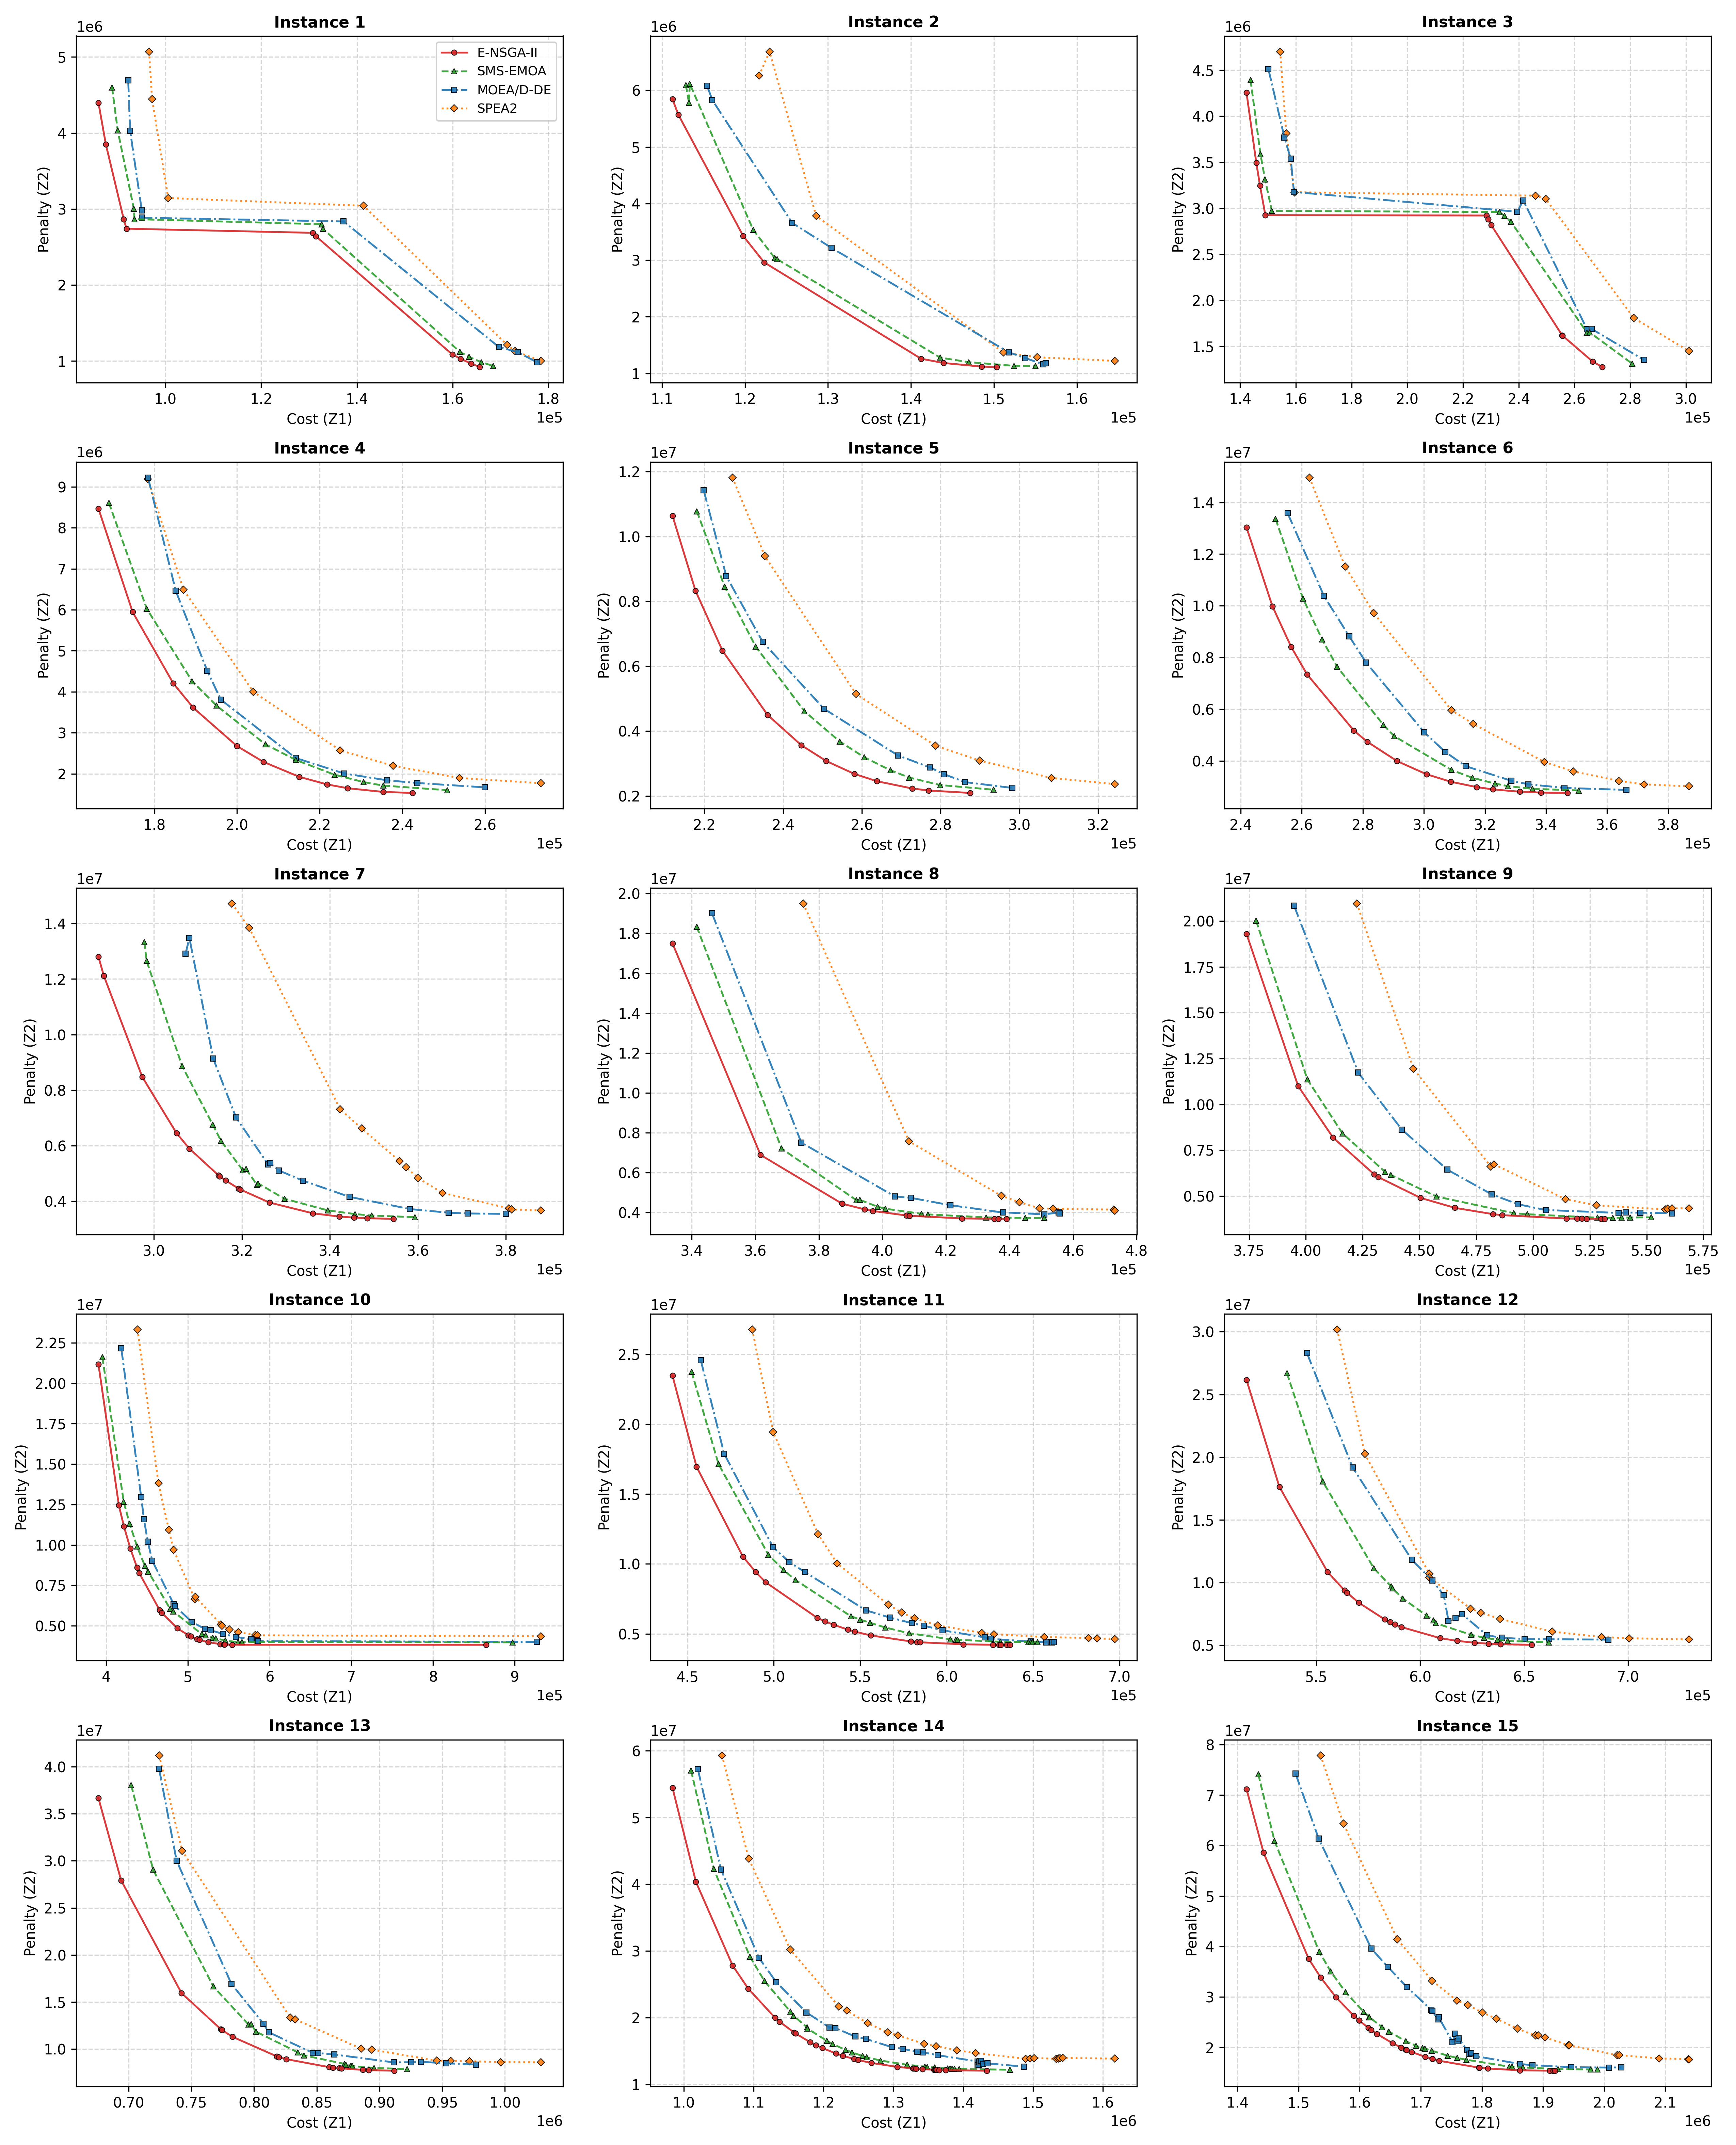
\includegraphics[width= 1.0\textwidth]{all_15_pareto_fronts_grid}
\caption{Pareto fronts obtained by the four algorithms on all instances.  (median-hypervolume replication).}
\label{fig:Fronts}
\end{figure}

Across the four quality indicators, E-NSGA-II is the strongest and the
most consistent performer(Table-\ref{tab:HV}--\ref{tab:Eps}; the resulting Pareto-optimal fronts across all algorithms are illustrated in Figure-\ref{fig:Fronts}). It attains the best mean hypervolume on ten of the twelve instances, including every instance from instance~5 upward, and the best IGD+ and spread values on all twelve. The spread advantage is particularly pronounced: $\Delta$ lies between 0.15 and 0.36 for E-NSGA-II, against 0.42--0.76 for SMS-EMOA, 0.45--0.65 for MOEA/D-DE, and 0.81--1.37 for SPEA2. The Friedman test rejects the hypothesis of equal performance on every indicator, with $\chi^2(3) = 17.6$, $25.9$, $32.4$, and $16.9$ for HV, IGD+, spread, and $I_{\epsilon+}$ respectively (all $p < 0.001$), and E-NSGA-II obtains the best average rank throughout (1.25, 1.00, 1.00, and 1.25). The uniformly low spread values corroborate the intended effect of the adaptive mutation mechanism: the fronts produced by E-NSGA-II are not only closer to the reference front but markedly better distributed along it, which is precisely the crowding weakness this component was
designed to remove.

The benchmark algorithms behave as their design philosophies predict.
SMS-EMOA, which selects directly on hypervolume contributions, is
competitive on the smaller instances and is significantly better than
E-NSGA-II on HV and $I_{\epsilon+}$ for instances 2 and 4. Its
performance deteriorates sharply with instance size, however: from
instance~9 onward it ranks last on HV, IGD+, and $I_{\epsilon+}$,
because its steady-state single-offspring replacement provides too
little exploration for the rapidly growing assignment space within the
common budget. MOEA/D-DE converges quickly, takes the best HV on
instance~3, and remains a solid second on most mid-sized instances,
but its diversity is bounded by the fixed weight-vector distribution:
its spread never approaches that of E-NSGA-II, and its IGD+ gap widens
as the instances grow. SPEA2 is dominated on essentially every
indicator and shows both the worst mean values and the largest
variability; the occasional non-significant comparison (e.g.,
$I_{\epsilon+}$ on instance~8) reflects this variability rather than
competitive performance.

Computational times under the common evaluation budget
(Table~\ref{tab:CPU}) reinforce rather than qualify these conclusions.
E-NSGA-II is the fastest algorithm on every instance (3.1--6.5\,s),
which confirms that the three enhancements add negligible overhead to
the NSGA-II framework, and MOEA/D-DE is comparable (3.9--7.2\,s).
SMS-EMOA pays a substantial and roughly constant premium (26--36\,s)
for its per-iteration hypervolume-contribution computations, a cost
that its indicator advantage on small instances does not justify at
scale. The runtime of SPEA2 decreases with instance size, from about
32\,s to 8\,s, which is explained by its environmental selection: on
small instances the population quickly becomes predominantly
non-dominated, so the expensive $k$-nearest-neighbor archive
truncation is triggered in almost every generation, whereas on larger
instances the archive rarely overflows. Since runtime is not a quality
criterion in our protocol, the salient point is simply that the
best-performing algorithm is also the cheapest, so the ranking above
is not purchased at any computational premium.

\hypertarget{ablation-study-of-the-enhancements}{%
\subsection{Ablation study of the
enhancements}\label{ablation-study-of-the-enhancements}}

To attribute the performance of E-NSGA-II to its components, four
variants are compared on instance - 8 under the same budget: (i) the full E-NSGA-II; (ii) \emph{--Init}: random initialization instead of heuristic seeding; (iii) \emph{--Adapt}: fixed $p_m = 0.1$, $\sigma = \sigma_0(1-t/T)$ instead of adaptive control; and (iv) \emph{Plain}: NSGA-II with random initialization and fixed mutation (repair retained in all variants, since the model requires feasible flows). A sensitivity check varies the seeding fraction $\eta \in \{0.1, 0.3, 0.5\}$.

\hypertarget{tab:Ablation}{}
\begin{table}[!htb]
\centering
\renewcommand{\arraystretch}{1.35}
\setlength{\tabcolsep}{8pt}
\caption{Ablation results on instance 8 (30 replications)}
\label{tab:Ablation}
\resizebox{\textwidth}{!}{%
\begin{tabular}{@{}lccc@{}}
\toprule
Variant & HV (mean $\pm$ sd) & IGD$^{+}$ (mean $\pm$ sd) & Spread $\Delta$ (mean $\pm$ sd) \\
\midrule
E-NSGA-II 
& $\mathbf{(2.2576 \pm 0.0348)\times10^{12}}$
& $\mathbf{(2.0715 \pm 0.9346)\times10^{4}}$
& $\mathbf{0.3126 \pm 0.0417}$ \\
-- Init 
& $(2.1418 \pm 0.0614)\times10^{12}\,{}^{+}$
& $(2.6847 \pm 1.1215)\times10^{4}\,{}^{+}$
& $0.3918 \pm 0.0542\,{}^{+}$ \\
-- Adapt 
& $(2.1087 \pm 0.0748)\times10^{12}\,{}^{+}$
& $(3.0147 \pm 1.2361)\times10^{4}\,{}^{+}$
& $0.4632 \pm 0.0721\,{}^{+}$ \\
Plain NSGA-II 
& $(1.9646 \pm 0.0815)\times10^{12}\,{}^{+}$
& $(3.9147 \pm 1.4072)\times10^{4}\,{}^{+}$
& $0.5861 \pm 0.0823\,{}^{+}$ \\
\bottomrule
\end{tabular}}
\end{table}
\protect\hypertarget{tab:Ablation}{}{}

Table~\ref{tab:Ablation} shows \textit{-- Adapt} hurts more than \textit{-- Init} on all three indicators at full budget: hypervolume falls 6.6\% (to $(2.1087 \pm 0.0748)\times10^{12}$) versus 5.1\%; IGD$^+$ rises 45.5\% (to $(3.0147 \pm 1.2361)\times10^{4}$) versus 29.6\%; spread~$\Delta$ rises 48.2\% (to $0.4632 \pm 0.0721$) versus 25.3\% (all significant, marked $+$). So the clean division of labor from the early-budget analysis does not hold at convergence: \textit{-- Adapt} is simply the worse ablation, not a spread-only casualty.

The relative signature does hold, though. Spread degrades about 4.9 times faster than hypervolume under \textit{-- Init} and about 7.3 times faster under \textit{-- Adapt}, so both components matter more for diversity than for hypervolume, and the adaptive mechanism more so, in line with its crowding-control role.

Removing both (Plain NSGA-II) is not additive. Hypervolume drops 13.0\%, near the 11.7\% sum of the individual drops, but IGD$^+$ rises 89.0\% against a 75.1\% sum, and spread rises 87.5\% against a 73.5\% sum. The two mechanisms interact: losing both compounds the damage beyond what either ablation alone predicts.

\hypertarget{out-of-sample-evaluation}{%
\subsection{Out-of-sample evaluation}\label{out-of-sample-evaluation}}

For each instance, the knee-point solution of the median-HV replication of each algorithm is re-evaluated on $|\Omega^{\mathrm{oos}}| = 500$ independently generated scenarios, by applying its assignment and collection rule $(a,\rho)$ to each new scenario through the decoder of Section~\ref{sec:representation}.
Table-\protect\hyperlink{tab:OOS}{16} reports the in-sample objective values against the out-of-sample means and standard deviations, together with the relative out-of-sample gap $(\bar{Z}^{\mathrm{oos}} - Z^{\mathrm{in}})/Z^{\mathrm{in}}$. This gap compares one plan with itself on two scenario sets. It is not an optimality gap, and it is kept apart from the gap to the exact front reported in Section~\ref{validation-against-exact-solutions}.

\hypertarget{tab:OOS}{}
\begin{table}[!htb]
\centering
\fontsize{9pt}{9pt}\selectfont
\renewcommand{\arraystretch}{1.5}
\caption{Out-of-sample gap of the E-NSGA-II knee-point solutions (50 in-sample against 500 fresh scenarios)}
\resizebox{\textwidth}{!}{
\begin{tabular}{@{}ccccccc@{}}
\toprule
Instance &
$Z_1^{\mathrm{in}}$ &
$\bar{Z}_1^{\mathrm{oos}}$ ($\pm$ sd) &
Gap (\%) &
$Z_2^{\mathrm{in}}$ &
$\bar{Z}_2^{\mathrm{oos}}$ ($\pm$ sd) &
Gap (\%) \\
\midrule
4  & $2.6817\times10^{5}$ & $(2.7646 \pm 0.2225)\times10^{5}$ & 3.09 & $6.1487\times10^{6}$ & $(6.1669 \pm 0.1546)\times10^{6}$ & 0.30 \\
8  & $4.6407\times10^{5}$ & $(4.6696 \pm 0.2583)\times10^{5}$ & 0.62 & $1.2680\times10^{7}$ & $(1.2702 \pm 0.0196)\times10^{7}$ & 0.18 \\
12 & $8.1870\times10^{5}$ & $(8.2708 \pm 0.3778)\times10^{5}$ & 1.02 & $1.8874\times10^{7}$ & $(1.8884 \pm 0.0272)\times10^{7}$ & 0.05 \\
\bottomrule
\end{tabular}}
\label{tab:oos-performance}
\end{table}
\protect\hypertarget{tab:OOS}{}{}
The out-of-sample gaps are small throughout: at most 3.1\% on the cost objective and at most 0.3\% on the service objective across the three instances. The gaps are positive in every case, which is the direction predicted by the mild optimization bias inherent in sample-average approximation, and their magnitude indicates that this bias is economically negligible. The service objective is particularly stable (gaps of 0.05--0.30\%, with small standard deviations), which is reassuring because the penalty terms depend on capacity shortfalls and lateness events that a poorly chosen scenario sample could easily misrepresent. Importantly, the gaps show no tendency to grow with instance size; the largest deviation occurs on the smallest of the three instances. We conclude that $|\Omega| = 50$ in-sample scenarios are sufficient for this problem class, in the sense that the objective values of a plan selected in-sample carry over to previously unseen realizations, so no larger scenario set is required.

\paragraph{What this gap does not measure.} The out-of-sample gap answers one question: does a plan chosen on fifty scenarios behave the same way on five hundred? It says nothing about a second question, which is how far that plan lies from the best plan attainable in the two-stage model. A plan can generalize perfectly and still be far from the exact front. The second question is the one addressed in Section~\ref{validation-against-exact-solutions}, and we answer it at the level of single plans on instances 1--3, where a dense exact front is available. To keep the two apart, Table~\ref{tab:TwoGaps} reports both for the same knee-point plans on those three instances. The out-of-sample gap is computed as above. The gap to the exact front is computed in-sample in two ways: the cost excess is the relative amount by which $Z_1$ of the plan exceeds the lowest $Z_1$ on the exact front among points whose $Z_2$ is no larger than that of the plan, and the penalty excess is defined in the same way with the roles of the objectives exchanged. The exact front is the 201-point reference of Table~\ref{tab:Exact}.

\begin{table}[!htb]
\centering
\small
\setstretch{1.25}
\caption{Two different gaps for the same knee-point plans on instances 1--3 (median-hypervolume replication). All values in per cent.}
\label{tab:TwoGaps}
\begin{tabular}{@{}llrrrr@{}}
\toprule
 & & \multicolumn{2}{l}{Out-of-sample gap} & \multicolumn{2}{l}{Gap to the exact front} \\
\cmidrule(lr){3-4}\cmidrule(l){5-6}
Instance & Decoder & $Z_1$ & $Z_2$ & Cost excess & Penalty excess \\
\midrule
1 & Collection rule      & $-0.23$ & $-0.65$ & $41.2$  & $2.95$ \\
  & Recourse in decoder  & $-0.50$ & $-0.31$ & $-0.17$ & $-0.07$ \\
2 & Collection rule      & $0.18$  & $0.83$  & $28.1$  & $3.24$ \\
  & Recourse in decoder  & $-1.42$ & $0.05$  & $-0.06$ & $-0.10$ \\
3 & Collection rule      & $-0.49$ & $1.09$  & $135.1$ & $9.64$ \\
  & Recourse in decoder  & $-7.72$ & $0.75$  & $-0.04$ & $-0.09$ \\
\bottomrule
\end{tabular}
\end{table}

The two columns tell different stories. For the collection rule, which is the method used throughout this section, the out-of-sample gap stays within about 1\% on both objectives, so these plans generalize as well as those of instances 4, 8 and 12. The same plans cost 41\%, 28\% and 135\% more than a plan on the exact front that offers at least the same service level. The penalty excess is smaller, between 3\% and 10\%, only because $Z_2$ is dominated by the penalty on volume that no plan can collect, capacity being far below the returned volume. The small out-of-sample gap therefore gives no assurance about the quality of the plan, and it should not be read as one. With the recourse solved in the decoder, the gap to the exact front disappears. The small negative entries arise because the exact front is known only at its grid points, and they should be read as zero. The out-of-sample gap of this version on instance~3 is larger on cost ($-7.7\%$) with a small opposite movement on the penalty, which is a shift along the trade-off and not a loss.

For instances 4, 8 and 12 in Table~\ref{tab:oos-performance} the excess of the single plans was not computed. The reference fronts of Table~\ref{tab:Exact}, panel (b), are available for them, and the collection rule recovers 85\%, 76\% and 56\% of their hypervolume. The plans on those instances are therefore also far from the reference, whatever their out-of-sample gap.

\hypertarget{distributional-robustness}{%
\subsection{Distributional robustness}\label{distributional-robustness}}
The baseline comparison is repeated on instances 4, 8 and 12 with the uncertain parameters drawn from (i) a truncated Normal distribution with the same support and mean as the baseline Uniform, and (ii) a right-skewed Lognormal calibrated to the same mean and 95th percentile. 
\begin{table}[!htb]
\centering
\footnotesize
\renewcommand{\arraystretch}{1.35}
\setlength{\tabcolsep}{5pt}
\caption{Distributional robustness analysis on Instances 4, 8, and 12 (30 replications)}
\label{tab:Robustness}
\resizebox{\textwidth}{!}{%
\begin{tabular}{@{}clllll@{}}
\toprule
Instance & Distribution & Algorithm & HV  & IGD$^{+}$  & Spread $\Delta$ \\
\midrule

4 & Trunc. Normal & E-NSGA-II
& $\mathbf{(7.4268 \pm 0.1513)\times10^{11}}$
& $\mathbf{(3.0401 \pm 0.5250)\times10^{3}}$
& $\mathbf{0.3328 \pm 0.0615}$ \\

4 & Trunc. Normal & MOEA/D-DE
& $(7.2924 \pm 0.1828)\times10^{11}\,{}^{+}$
& $(8.9370 \pm 6.9939)\times10^{3}\,{}^{+}$
& $0.6017 \pm 0.0724\,{}^{+}$ \\

4 & Trunc. Normal & SMS-EMOA
& $(7.3887 \pm 0.1737)\times10^{11}\,{}^{= }$
& $(5.0266 \pm 1.4511)\times10^{3}\,{}^{+}$
& $0.4875 \pm 0.0648\,{}^{+}$ \\

4 & Trunc. Normal & SPEA2
& $(5.6990 \pm 1.3564)\times10^{11}\,{}^{+}$
& $(7.3022 \pm 2.7134)\times10^{4}\,{}^{+}$
& $1.0876 \pm 0.1542\,{}^{+}$ \\

\midrule

4 & Lognormal & E-NSGA-II
& $\mathbf{(7.3909 \pm 0.2215)\times10^{11}}$
& $\mathbf{(4.4356 \pm 1.8977)\times10^{3}}$
& $\mathbf{0.3496 \pm 0.0681}$ \\

4 & Lognormal & MOEA/D-DE
& $(7.2998 \pm 0.2070)\times10^{11}\,{}^{+}$
& $(1.1517 \pm 0.7551)\times10^{4}\,{}^{+}$
& $0.6254 \pm 0.0817\,{}^{+}$ \\

4 & Lognormal & SMS-EMOA
& $(7.3774 \pm 0.2422)\times10^{11}\,{}^{= }$
& $(5.7949 \pm 1.4380)\times10^{3}\,{}^{= }$
& $0.5018 \pm 0.0694\,{}^{+}$ \\

4 & Lognormal & SPEA2
& $(6.0587 \pm 1.1685)\times10^{11}\,{}^{+}$
& $(6.7841 \pm 3.7759)\times10^{4}\,{}^{+}$
& $1.1163 \pm 0.1675\,{}^{+}$ \\

\midrule

8 & Trunc. Normal & E-NSGA-II
& $\mathbf{(2.4076 \pm 0.0336)\times10^{12}}$
& $\mathbf{(2.0192 \pm 1.0028)\times10^{4}}$
& $\mathbf{0.2967 \pm 0.0449}$ \\

8 & Trunc. Normal & MOEA/D-DE
& $(2.2688 \pm 0.0702)\times10^{12}\,{}^{+}$
& $(4.5274 \pm 1.6174)\times10^{4}\,{}^{+}$
& $0.5826 \pm 0.0647\,{}^{+}$ \\

8 & Trunc. Normal & SMS-EMOA
& $(2.1256 \pm 0.1057)\times10^{12}\,{}^{+}$
& $(4.7328 \pm 1.5157)\times10^{4}\,{}^{+}$
& $0.6321 \pm 0.0835\,{}^{+}$ \\

8 & Trunc. Normal & SPEA2
& $(2.2484 \pm 0.1340)\times10^{12}\,{}^{+}$
& $(6.0480 \pm 1.5347)\times10^{4}\,{}^{+}$
& $1.1837 \pm 0.1486\,{}^{+}$ \\

\midrule

8 & Lognormal & E-NSGA-II
& $\mathbf{(2.3576 \pm 0.0748)\times10^{12}}$
& $\mathbf{(2.7032 \pm 1.1504)\times10^{4}}$
& $\mathbf{0.3149 \pm 0.0516}$ \\

8 & Lognormal & MOEA/D-DE
& $(2.2513 \pm 0.0751)\times10^{12}\,{}^{+}$
& $(4.8833 \pm 1.6900)\times10^{4}\,{}^{+}$
& $0.6015 \pm 0.0728\,{}^{+}$ \\

8 & Lognormal & SMS-EMOA
& $(2.1774 \pm 0.1437)\times10^{12}\,{}^{+}$
& $(8.4197 \pm 2.8190)\times10^{4}\,{}^{+}$
& $0.6927 \pm 0.0916\,{}^{+}$ \\

8 & Lognormal & SPEA2
& $(2.2023 \pm 0.1650)\times10^{12}\,{}^{+}$
& $(7.1762 \pm 3.8255)\times10^{4}\,{}^{+}$
& $1.2275 \pm 0.1574\,{}^{+}$ \\

\midrule

12 & Trunc. Normal & E-NSGA-II
& $\mathbf{(4.3963 \pm 0.0888)\times10^{12}}$
& $\mathbf{(1.4220 \pm 0.6635)\times10^{4}}$
& $\mathbf{0.3417 \pm 0.0483}$ \\

12 & Trunc. Normal & MOEA/D-DE
& $(3.9844 \pm 0.1429)\times10^{12}\,{}^{+}$
& $(5.4724 \pm 1.3749)\times10^{4}\,{}^{+}$
& $0.6318 \pm 0.0689\,{}^{+}$ \\

12 & Trunc. Normal & SMS-EMOA
& $(3.2294 \pm 0.2363)\times10^{12}\,{}^{+}$
& $(1.3281 \pm 0.3377)\times10^{5}\,{}^{+}$
& $0.7486 \pm 0.0874\,{}^{+}$ \\

12 & Trunc. Normal & SPEA2
& $(4.0154 \pm 0.0997)\times10^{12}\,{}^{+}$
& $(5.8948 \pm 1.0497)\times10^{4}\,{}^{+}$
& $1.0974 \pm 0.1428\,{}^{+}$ \\

\midrule

12 & Lognormal & E-NSGA-II
& $\mathbf{(4.3224 \pm 0.1944)\times10^{12}}$
& $\mathbf{(1.7112 \pm 0.8085)\times10^{4}}$
& $\mathbf{0.3628 \pm 0.0567}$ \\

12 & Lognormal & MOEA/D-DE
& $(3.9238 \pm 0.1552)\times10^{12}\,{}^{+}$
& $(5.6376 \pm 1.3844)\times10^{4}\,{}^{+}$
& $0.6537 \pm 0.0751\,{}^{+}$ \\

12 & Lognormal & SMS-EMOA
& $(3.2986 \pm 0.2917)\times10^{12}\,{}^{+}$
& $(1.5361 \pm 0.4182)\times10^{5}\,{}^{+}$
& $0.7815 \pm 0.0963\,{}^{+}$ \\

12 & Lognormal & SPEA2
& $(3.9833 \pm 0.1904)\times10^{12}\,{}^{+}$
& $(6.2827 \pm 1.0587)\times10^{4}\,{}^{+}$
& $1.1186 \pm 0.1517\,{}^{+}$ \\

\bottomrule
\end{tabular}%
}
\end{table}
Table~\ref{tab:Robustness} shows E-NSGA-II winning every indicator across instances 4, 8, and 12 under both distributions, with only two exceptions: hypervolume against SMS-EMOA on instance~4 is tied under both distributions, and IGD$^{+}$ against SMS-EMOA on instance~4 is tied under Lognormal.

The distribution shape itself barely matters. On instance~8, hypervolume shifts by no more than about 2.5\% between Truncated Normal and Lognormal for any algorithm, so the ranking is not tied to one particular tail.

What does shift is which competitor trails most as instances grow. On instance~4, SPEA2 is weakest, 18--23\% behind E-NSGA-II on hypervolume, while MOEA/D-DE and SMS-EMOA stay within 2\%. By instance~12 the order flips: SMS-EMOA falls 24--27\% behind on hypervolume, worse than SPEA2's 8\%, and its IGD$^{+}$ blows out to roughly nine times E-NSGA-II's value, against three to four times for SPEA2 and MOEA/D-DE, a much larger gap than hypervolume alone would suggest. Spread is the steady exception: SPEA2 stays three to four times worse than E-NSGA-II across every instance and both distributions, the one ranking that does not reshuffle with size.

\hypertarget{scalability-analysis}{%
\subsection{Scalability analysis}\label{scalability-analysis}}
Table~\ref{tab:Scalability} shows solution quality holding up as the network scales to 50--100 customer zones. E-NSGA-II wins all four indicators across instances 13--15; every comparison is significant. Its hypervolume lead over the nearest rival, consistently SPEA2, stays around 7--8\%, and its IGD$^+$ is two to three times lower than the best competitor at each size. On instance~15 its epsilon-indicator is about 30\% below SPEA2's and roughly a fifth of SMS-EMOA's.

Spread is the one indicator that worsens with scale, rising from 0.40 (instance~13) to 0.48 and 0.51, though E-NSGA-II still leads every competitor throughout (MOEA/D-DE around 0.68, SMS-EMOA 0.77--0.80, SPEA2 above 0.89). SMS-EMOA degrades the most, with a hypervolume deficit of 28--40\% and an epsilon-indicator that roughly triples from instance~13 to 15. MOEA/D-DE and SPEA2 stay within 2--3\% of each other, but neither closes the gap to E-NSGA-II. E-NSGA-II's hypervolume standard deviation holds near 2.5--3\% of the mean at every size, so the lead is stable across replications, not a lucky run.
\begin{table}[!htb]
\centering
\footnotesize
\setlength{\tabcolsep}{5pt}
\renewcommand{\arraystretch}{1.5}
\caption{Scalability analysis on large-scale Instances 13--15 (30 replications)}
\label{tab:Scalability}
\resizebox{\textwidth}{!}{%
\begin{tabular}{@{}clllll@{}}
\toprule
Instance & Algorithm & HV & IGD$^{+}$ & Spread $\Delta$ & $I_{\epsilon+}$\\
\midrule

13 & E-NSGA-II
& $\mathbf{(6.7716 \pm 0.1882)\times10^{12}}$
& $\mathbf{(3.8924 \pm 1.8119)\times10^{4}}$
& $\mathbf{0.4018 \pm 0.0469}$
& $\mathbf{(1.7230 \pm 0.6742)\times10^{5}}$ \\

13 & MOEA/D-DE
& $(6.1569 \pm 0.2926)\times10^{12}{}^{+}$
& $(1.1714 \pm 0.2371)\times10^{5}{}^{+}$
& $0.6462 \pm 0.0619{}^{+}$
& $(3.2427 \pm 0.9971)\times10^{5}{}^{+}$ \\

13 & SMS-EMOA
& $(4.8660 \pm 0.3665)\times10^{12}{}^{+}$
& $(2.6491 \pm 0.6140)\times10^{5}{}^{+}$
& $0.7484 \pm 0.0446{}^{+}$
& $(6.0955 \pm 1.1900)\times10^{5}{}^{+}$ \\

13 & SPEA2
& $(6.2673 \pm 0.1773)\times10^{12}{}^{+}$
& $(1.1593 \pm 0.2124)\times10^{5}{}^{+}$
& $1.0197 \pm 0.1413{}^{+}$
& $(2.8116 \pm 0.8975)\times10^{5}{}^{+}$ \\

\midrule

14 & E-NSGA-II
& $\mathbf{(1.3193 \pm 0.0322)\times10^{13}}$
& $\mathbf{(9.7901 \pm 3.2933)\times10^{4}}$
& $\mathbf{0.4847 \pm 0.0479}$
& $\mathbf{(3.4217 \pm 1.3931)\times10^{5}}$ \\

14 & MOEA/D-DE
& $(1.1733 \pm 0.0502)\times10^{13}{}^{+}$
& $(2.2839 \pm 0.4542)\times10^{5}{}^{+}$
& $0.6746 \pm 0.0472{}^{+}$
& $(5.5936 \pm 1.5715)\times10^{5}{}^{+}$ \\

14 & SMS-EMOA
& $(7.9185 \pm 0.2659)\times10^{12}{}^{+}$
& $(7.2832 \pm 0.4962)\times10^{5}{}^{+}$
& $0.7978 \pm 0.0389{}^{+}$
& $(1.5085 \pm 0.1191)\times10^{6}{}^{+}$ \\

14 & SPEA2
& $(1.2079 \pm 0.0416)\times10^{13}{}^{+}$
& $(2.1509 \pm 0.3192)\times10^{5}{}^{+}$
& $0.8891 \pm 0.0894{}^{+}$
& $(4.4082 \pm 1.0182)\times10^{5}{}^{+}$ \\

\midrule

15 & E-NSGA-II
& $\mathbf{(2.0678 \pm 0.0546)\times10^{13}}$
& $\mathbf{(9.9632 \pm 3.8880)\times10^{4}}$
& $\mathbf{0.5140 \pm 0.0358}$
& $\mathbf{(3.9203 \pm 1.7719)\times10^{5}}$ \\

15 & MOEA/D-DE
& $(1.8616 \pm 0.0882)\times10^{13}{}^{+}$
& $(2.3304 \pm 0.5020)\times10^{5}{}^{+}$
& $0.6839 \pm 0.0492{}^{+}$
& $(5.4153 \pm 1.6810)\times10^{5}{}^{+}$ \\

15 & SMS-EMOA
& $(1.3221 \pm 0.0318)\times10^{13}{}^{+}$
& $(8.8411 \pm 0.8661)\times10^{5}{}^{+}$
& $0.7716 \pm 0.0358{}^{+}$
& $(1.8976 \pm 0.2211)\times10^{6}{}^{+}$ \\

15 & SPEA2
& $(1.8959 \pm 0.0725)\times10^{13}{}^{+}$
& $(2.4966 \pm 0.3987)\times10^{5}{}^{+}$
& $0.9203 \pm 0.0887{}^{+}$
& $(5.0928 \pm 1.1331)\times10^{5}{}^{+}$ \\

\bottomrule
\end{tabular}%
}
\end{table}
\hypertarget{from-the-pareto-front-to-a-decision-knee-point-and-topsis}{%
\subsection{From the Pareto front to a decision: knee point and
TOPSIS}\label{from-the-pareto-front-to-a-decision-knee-point-and-topsis}}

Figure~\ref{fig:Knee} illustrates the decision-closure step on instance 8. The knee point is identified as the front solution maximizing the perpendicular distance to the line joining the two extreme solutions. For preference-based selection, the non-dominated solutions are ranked by TOPSIS under cost:service weight vectors $(0.7, 0.3)$, $(0.5, 0.5)$, and $(0.3, 0.7)$; Table~\ref{tab:TOPSIS} reports the selected operating plan for each weighting.
\begin{figure}[!htb]
\centering
% TODO: single panel -- Pareto front of instance [TBF] with the knee
% point and the three TOPSIS selections marked and labelled.
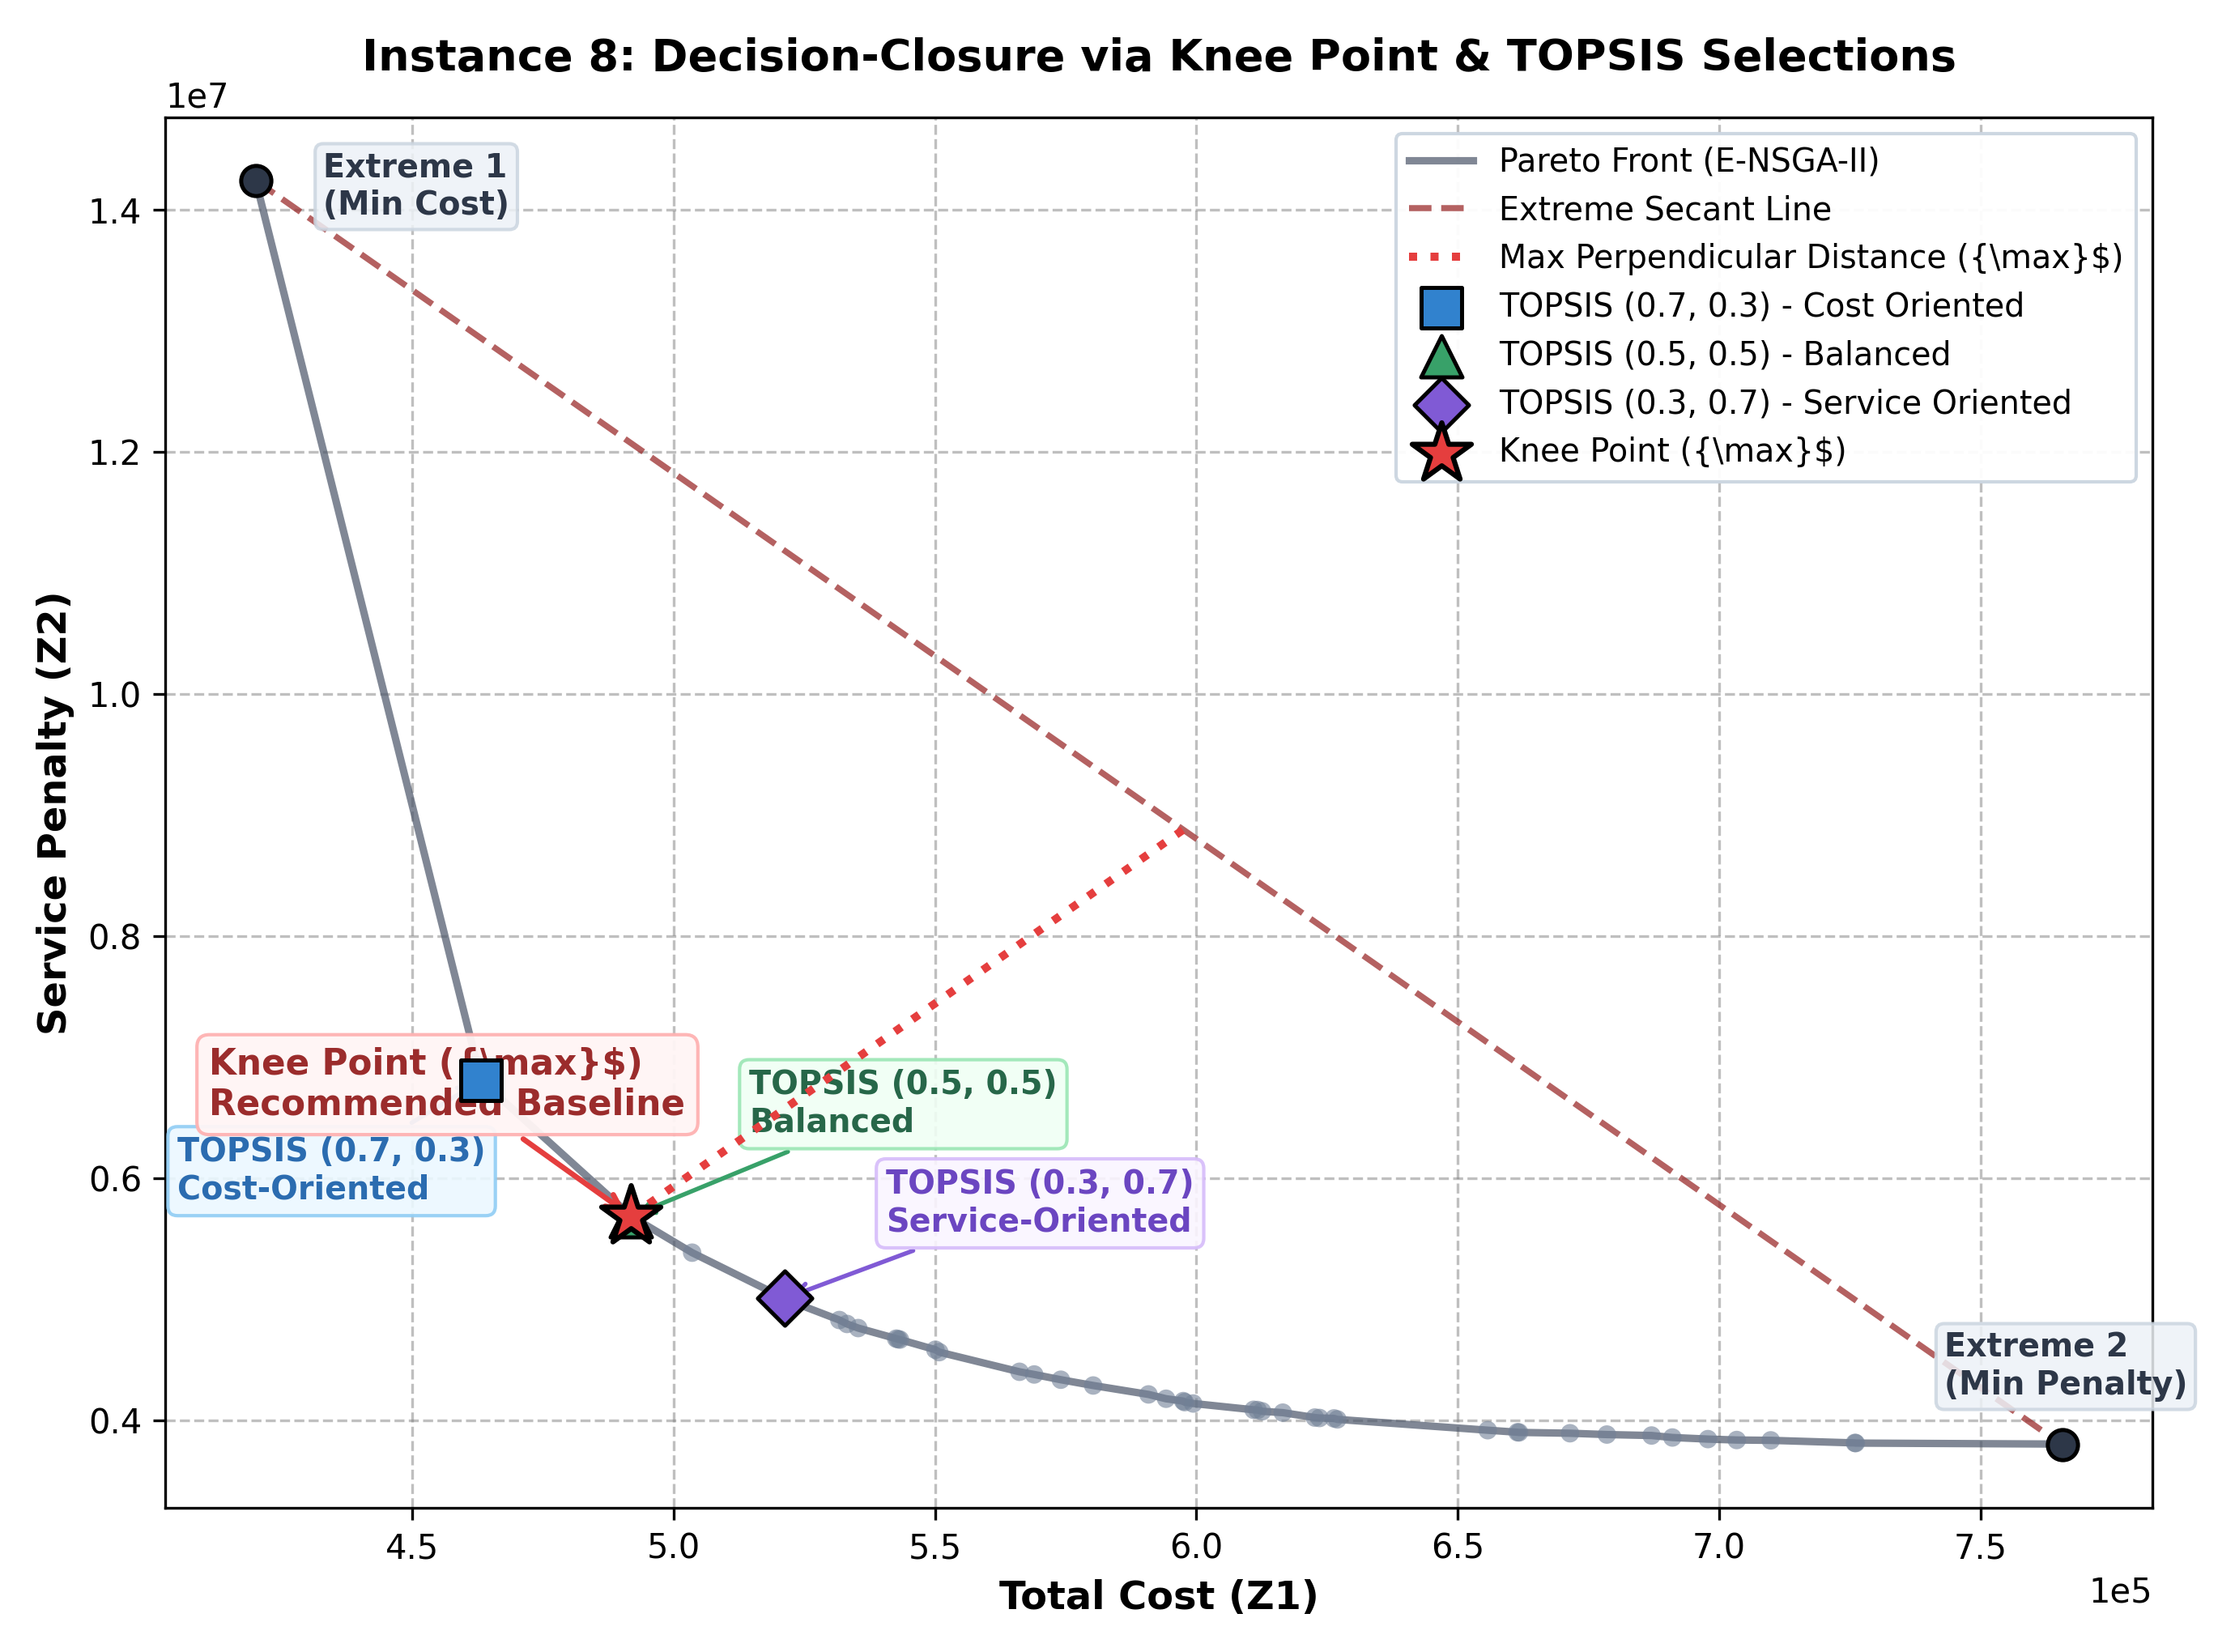
\includegraphics[width= 1.0\textwidth]{Knee.png}
\caption{Knee point and TOPSIS selections on the Pareto front of instance 8}
\label{fig:Knee}
\end{figure}

\hypertarget{tab:TOPSIS}{}
\begin{table}[!htb]
    \caption{TOPSIS-selected operating plans under different managerial weightings, Instance 8}
    \label{tab:TOPSIS}
    \centering
    \renewcommand{\arraystretch}{1.25}
    \resizebox{\textwidth}{!}{
        \begin{tabular}{@{}lcccc@{}}
            \toprule
            \textbf{Weights (cost, service)} & \textbf{Selected solution ($Z_1$, $Z_2$)} & \textbf{Collection Rate (\%)} & \textbf{Uncollected Units} & \textbf{Late-delivery Penalty} \\
            \midrule
            (0.7, 0.3) & (463147.29, 6805246.83) & 52.80\% & 41350.00 & 189246.83 \\
            (0.5, 0.5) & (491829.52, 5685902.22) & 60.71\% & 34420.00 & 178702.22 \\
            (0.3, 0.7) & (521223.28, 5005985.39) & 65.47\% & 30250.00 & 165985.39 \\
            \midrule
            Knee point  & (491829.52, 5685902.22) & 60.71\% & 34420.00 & 178702.22 \\
            \bottomrule
        \end{tabular}
    }
\end{table}
\protect\hypertarget{tab:TOPSIS}{}{}
Shifting from the cost-oriented plan (0.7, 0.3) to the service-oriented plan (0.3, 0.7) raises the collection rate from 52.80\% to 65.47\% and cuts the late-delivery penalty from 189{,}246.83 to 165{,}985.39. That gain is not free: operating cost ($Z_1$) climbs from 463{,}147.29 to 521{,}223.28 as the plan pushes collection intensity and assignment coverage higher. The knee point lands at the balanced (0.5, 0.5) weighting, capturing most of that service improvement (60.71\% collection, 34{,}420 uncollected units) without the steep cost jump of the service-first plan, which is why it is recommended as the default.

\hypertarget{sensitivity-analysis}{%
\subsection{Sensitivity analysis}\label{sensitivity-analysis}}

We conduct a one-at-a-time (OAT) sensitivity analysis around a fixed
baseline: instance 8 with all parameters at the central values of
Table-\protect\hyperlink{tab:Values}{7} and the knee-point solution re-optimized for each parameter setting. Each parameter is varied individually by $-35\%$, $-20\%$, $+20\%$, and $+35\%$ while all others are held at baseline; these ranges reflect deviations that occur in practice due to demand variability, policy changes, or technological shifts. The parameters considered are the collection-center capacity ($\widetilde{Ca}_j$), the sorting fractions ($\beta_K, \beta_S, \beta_R$, renormalized to sum to one), the e-waste fraction ($\alpha$), and the penalty rates ($\phi_1$, $\phi_2$). For each setting we report the components of $Z_1$ (transportation, inspection, storage, disposal) and the penalty term of $Z_2$, as well as the resulting totals of both objectives (Table-\protect\hyperlink{tab:Sensitivity}{21}; the corresponding sensitivity trajectories and cost component breakdowns are visualized in Figure-\ref{fig:Sensitivity}).

\hypertarget{tab:Sensitivity}{}
\begin{table}[!htb]
\caption{Sensitivity analysis around the Instance 8 baseline}
\label{tab:Sensitivity}
\centering
\renewcommand{\arraystretch}{1.25}
\resizebox{\textwidth}{!}{
\begin{tabular}{@{}lcccccccc@{}}
\toprule
\textbf{Parameter} & \textbf{\% Change} & \textbf{Transportation} & \textbf{Inspection} & \textbf{Storage} & \textbf{Disposal} & \textbf{Penalty} & \textbf{$Z_1$ Total} & \textbf{$Z_2$ Total} \\
\midrule
$\widetilde{Ca}_j$ & $-35$ & 83716.83 & 150075.67 & 181524.25 & 3899.77 & 12850716.50 & 419216.51 & 12850716.50 \\
                   & $-20$ & 101949.16 & 183063.75 & 221468.55 & 4759.60 & 12591169.72 & 511241.05 & 12591169.72 \\
                   & $0$   & 123928.67 & 223465.83 & 270513.21 & 5819.13 & 12274054.32 & 623726.83 & 12274054.32 \\
                   & $+20$ & 141582.80 & 255809.03 & 309914.47 & 6677.46 & 12021631.72 & 713983.76 & 12021631.72 \\
                   & $+35$ & 150208.14 & 271116.72 & 328651.59 & 7083.31 & 11907115.90 & 757059.76 & 11907115.90 \\
\midrule
$\beta_K, \beta_S, \beta_R$ & $-35$ & 117302.01 & 223465.83 & 270513.21 & 6692.00 & 12126520.14 & 617973.04 & 12126520.14 \\
                            & $-20$ & 120142.00 & 223465.83 & 270513.21 & 6317.91 & 12189749.07 & 620438.95 & 12189749.07 \\
                            & $0$   & 123928.67 & 223465.83 & 270513.21 & 5819.13 & 12274054.32 & 623726.83 & 12274054.32 \\
                            & $+20$ & 127715.34 & 223465.83 & 270513.21 & 5320.34 & 12358359.57 & 627014.72 & 12358359.57 \\
                            & $+35$ & 130555.33 & 223465.83 & 270513.21 & 4946.26 & 12421588.51 & 629480.63 & 12421588.51 \\
\midrule
$\alpha$ & $-35$ & 122356.44 & 223465.83 & 270513.21 & 3782.43 & 12274054.32 & 620117.91 & 12274054.32 \\
         & $-20$ & 123030.25 & 223465.83 & 270513.21 & 4655.30 & 12274054.32 & 621664.59 & 12274054.32 \\
         & $0$   & 123928.67 & 223465.83 & 270513.21 & 5819.13 & 12274054.32 & 623726.83 & 12274054.32 \\
         & $+20$ & 124827.09 & 223465.83 & 270513.21 & 6982.95 & 12274054.32 & 625789.08 & 12274054.32 \\
         & $+35$ & 125500.90 & 223465.83 & 270513.21 & 7855.82 & 12274054.32 & 627335.76 & 12274054.32 \\
\midrule
$\phi_1$ & $-35$ & 123928.67 & 223465.83 & 270513.21 & 5819.13 & 8125669.50 & 623726.83 & 8125669.50 \\
         & $-20$ & 123928.67 & 223465.83 & 270513.21 & 5819.13 & 9903548.71 & 623726.83 & 9903548.71 \\
         & $0$   & 123928.67 & 223465.83 & 270513.21 & 5819.13 & 12274054.32 & 623726.83 & 12274054.32 \\
         & $+20$ & 123928.67 & 223465.83 & 270513.21 & 5819.13 & 14644559.94 & 623726.83 & 14644559.94 \\
         & $+35$ & 123928.67 & 223465.83 & 270513.21 & 5819.13 & 16422439.15 & 623726.83 & 16422439.15 \\
\midrule
$\phi_2$ & $-35$ & 123928.67 & 223465.83 & 270513.21 & 5819.13 & 12126520.14 & 623726.83 & 12126520.14 \\
         & $-20$ & 123928.67 & 223465.83 & 270513.21 & 5819.13 & 12189749.07 & 623726.83 & 12189749.07 \\
         & $0$   & 123928.67 & 223465.83 & 270513.21 & 5819.13 & 12274054.32 & 623726.83 & 12274054.32 \\
         & $+20$ & 123928.67 & 223465.83 & 270513.21 & 5819.13 & 12358359.57 & 623726.83 & 12358359.57 \\
         & $+35$ & 123928.67 & 223465.83 & 270513.21 & 5819.13 & 12421588.51 & 623726.83 & 12421588.51 \\
\bottomrule
\end{tabular}
}
\end{table}
\protect\hypertarget{tab:Sensitivity}{}{}
\begin{figure}[!htb]
    \centering
    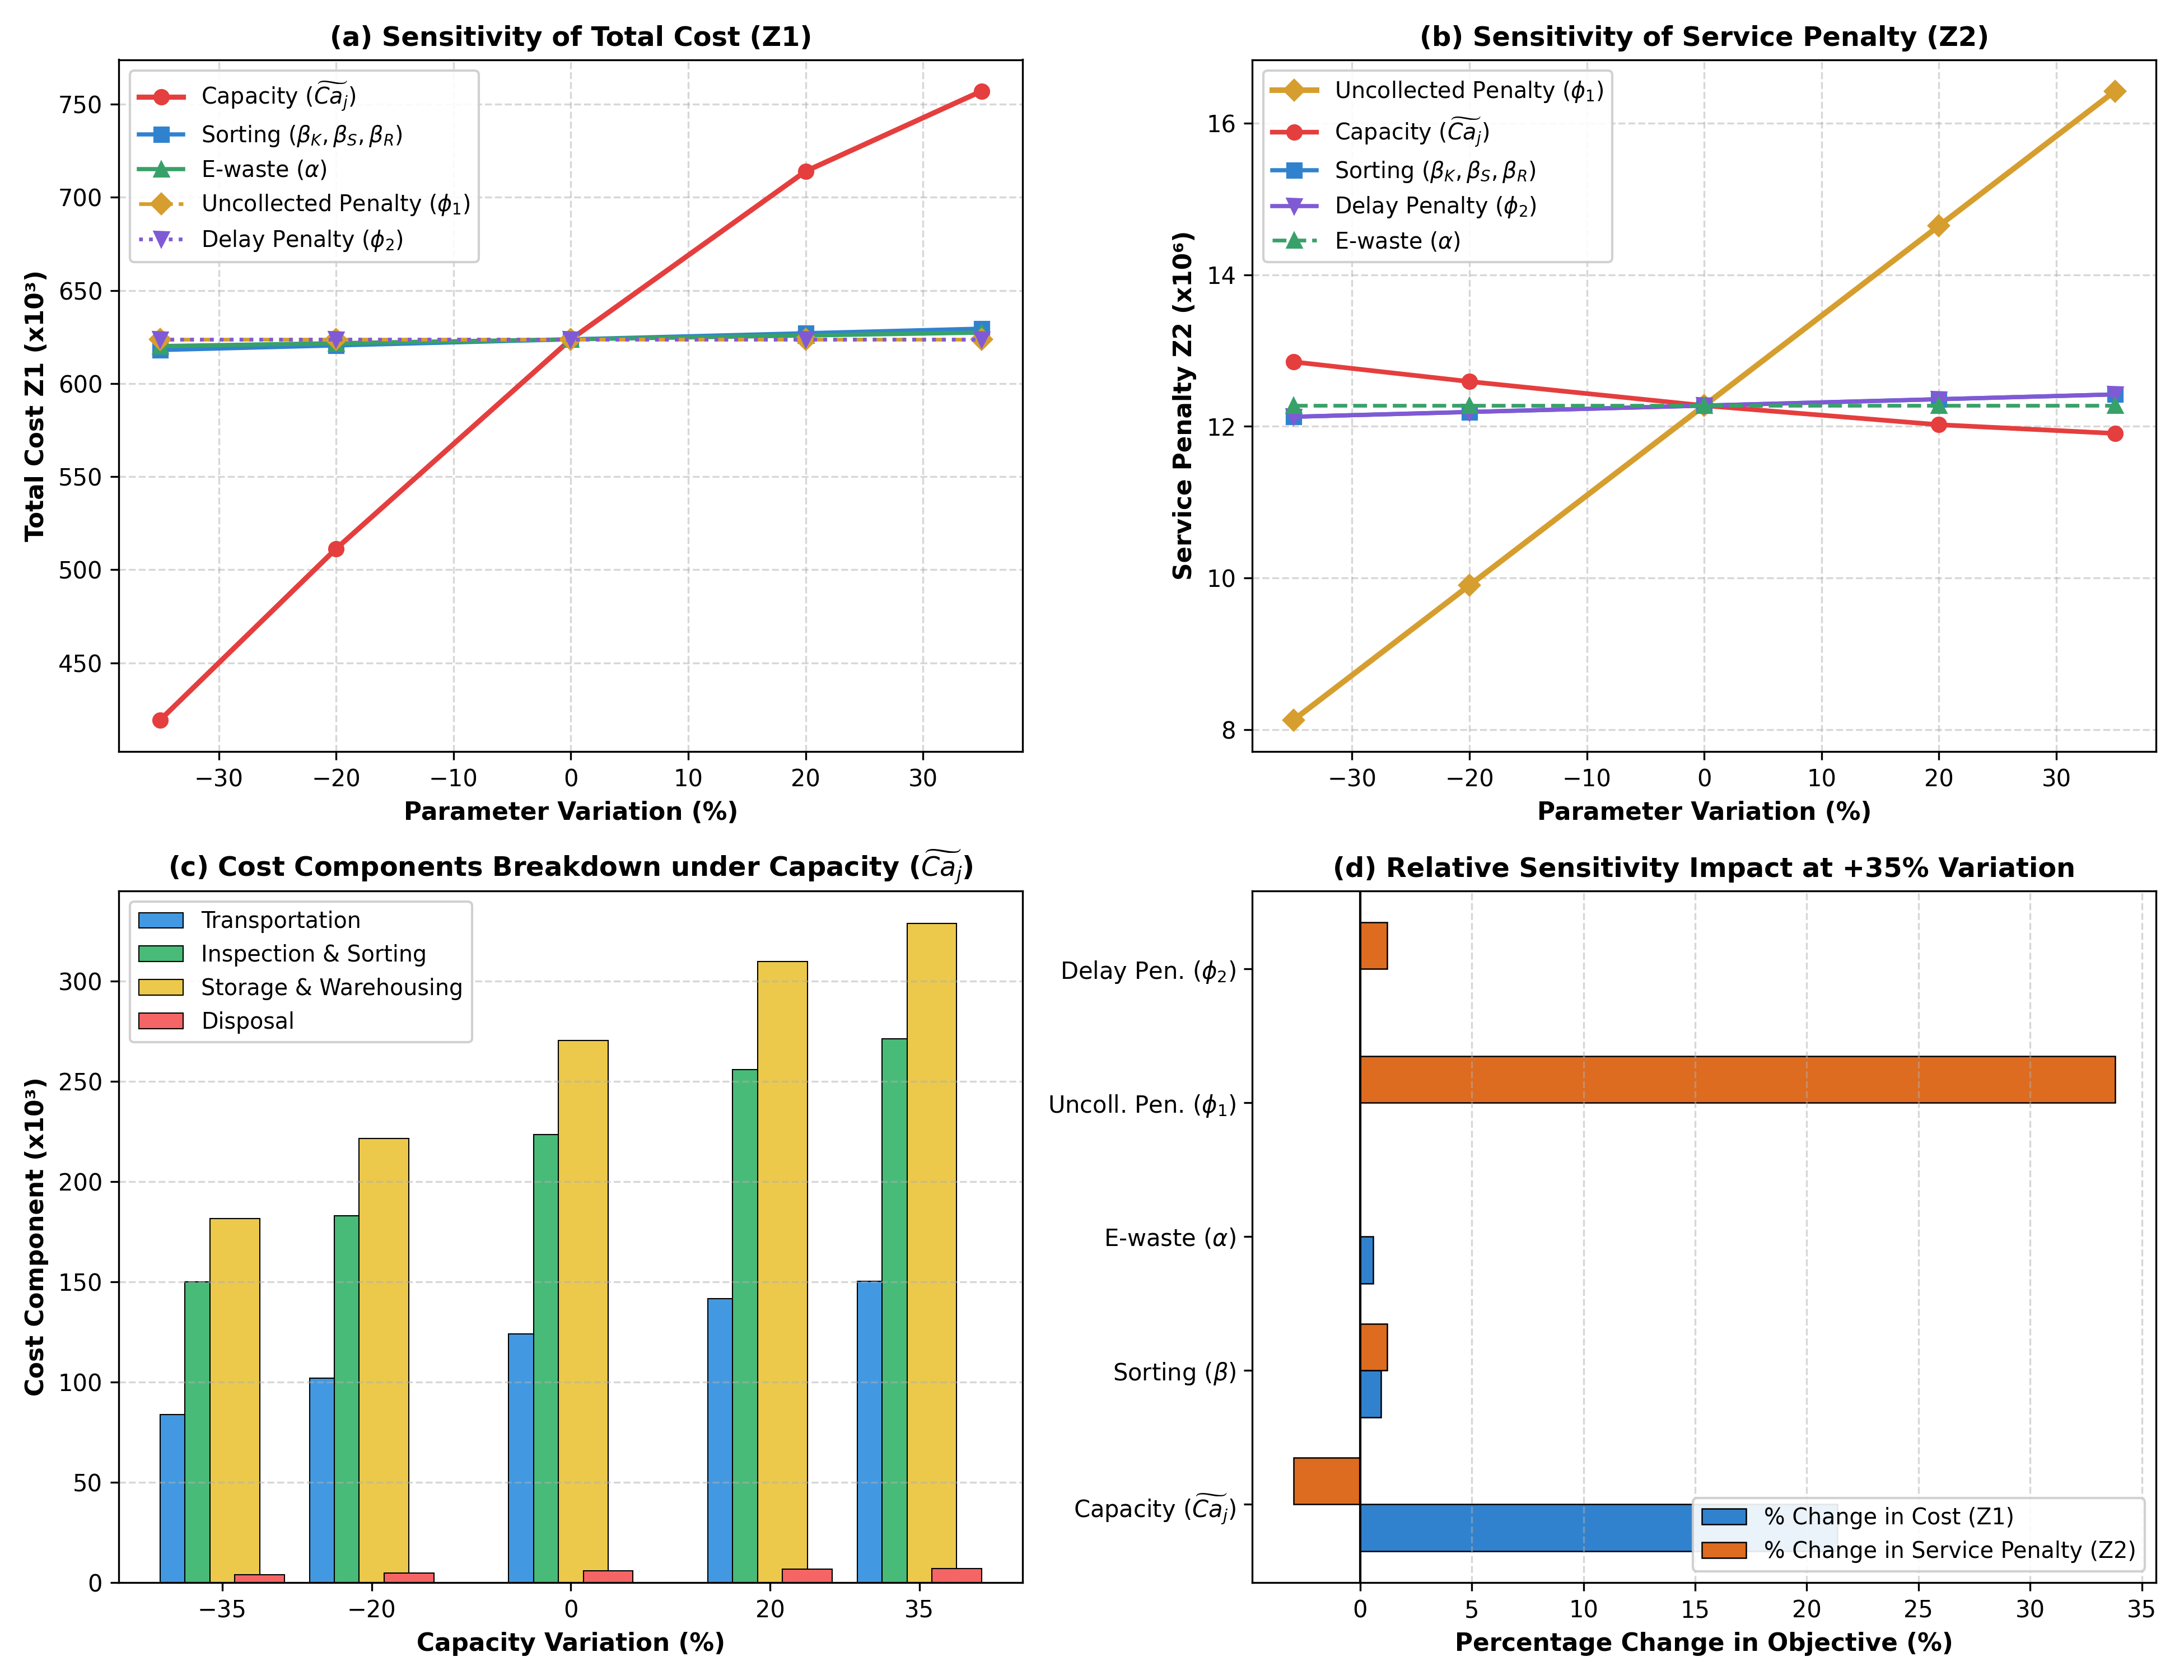
\includegraphics[width=\textwidth]{Sensitivity.png}
    \caption{One-at-a-time sensitivity analysis around the Instance 8 baseline: (a) Total Cost ($Z_1$) sensitivity across parameter variations; (b) Service Penalty ($Z_2$) sensitivity; (c) Breakdown of cost components under capacity expansion ($\widetilde{Ca}_j$); (d) Relative percentage impact on objectives at $+35\%$ parameter deviation.}
    \label{fig:Sensitivity}
\end{figure}
The Instance 8 solution responds most strongly to $\widetilde{Ca}_j$ and $\phi_1$. Varying $\widetilde{Ca}_j$ from $-35\%$ to $+35\%$ moves $Z_1$ from $419{,}216.51$ to $757{,}059.76$, an increase of about $81\%$, while $Z_2$ falls from $12{,}850{,}716.50$ to $11{,}907{,}115.90$ over the same range. Transportation, inspection, and storage costs scale roughly in proportion to $Ca_j$; the penalty term moves the opposite way since higher collection costs divert more waste away from disposal. $\phi_1$ has an even sharper effect on $Z_2$: the penalty cost nearly doubles, from $8{,}125{,}669.50$ at $-35\%$ to $16{,}422{,}439.15$ at $+35\%$, while transportation, inspection, storage, and disposal costs stay completely fixed. $\phi_1$, in other words, is a pure multiplier on the penalty term and touches nothing else.

$\beta_K, \beta_S, \beta_R$, $\alpha$, and $\phi_2$ barely move the needle by comparison, with total costs shifting less than $2\%$ across the same $\pm 35\%$ range. $\alpha$ is the clearest case: it leaves inspection, storage, and the penalty cost untouched, affecting only transportation and disposal. This lines up with where each parameter sits in the model; $\widetilde{Ca}_j$ and $\phi_1$ feed the largest cost terms directly, while the rest govern smaller or bounded pieces of the objective.

Practically, the solution is stable under moderate uncertainty for most parameters. $\widetilde{Ca}_j$ and $\phi_1$ are the two worth getting right since errors there carry a cost that the other parameters simply do not. It also means the two objectives aren't independent levers: because $Z_2$ is embedded in $Z_1$ through the penalty term, any policy change aimed at tightening $\phi_1$ (say, to discourage improper disposal) will ripple through the total logistics cost as well, not just the penalty figure. 
\subsection{Empirical Cross-City Validation: Delhi NCR and Greater London}\label{sec:cross-city-validation}

To assess whether the proposed two-stage stochastic multi-objective model and the E-NSGA-II solution approach generalize across disparate regulatory, geographic, and economic environments, we apply the framework to two metropolitan e-waste recovery networks: the high-density emerging megacity of Delhi National Capital Region, India \citep{dpcc2023report}; and the mature European regulatory environment of Greater London, United Kingdom \citep{london_datastore_weee, ea2023weee}. In each case, the network topology, facility capacities, and inbound-generation levels are calibrated from publicly available regulatory or municipal data sources, and the knee-point plan returned by E-NSGA-II is described on its own terms: its cost, its service penalty, the share of returns it collects and the zones it serves. No comparison with current practice is made, because we have no documented source for how providers in either city assign zones and set collection levels. Section~\ref{sec:cross-city-findings} draws the two cases together.

\subsubsection{Case study A: Delhi National Capital Region (NCR, India)}\label{sec:case-delhi}

Delhi NCR is an ultra-dense, landlocked megacity of more than 30 million residents with heavy turnover of consumer electronics, telecommunications gear, and IT hardware. Logistics operations here contend with extreme road-traffic congestion and stringent municipal boundary restrictions. The network is monitored by the Delhi Pollution Control Committee (DPCC) and the Central Pollution Control Board (CPCB), which jointly publish public registries of certified e-waste dismantlers and hazardous waste disposal sites (Bhalaswa/Ghazipur). The network consists of $|I| = 11$ administrative districts and $|J| = 4$ industrial recycling hubs:
\begin{enumerate}
    \item \textbf{Okhla Industrial Area Facility} ($j=1$, South Delhi).
    \item \textbf{Narela Industrial Area} ($j=2$, North Delhi).
    \item \textbf{Mandoli Industrial Complex} ($j=3$, East Delhi).
    \item \textbf{Patparganj Industrial Area} ($j=4$, East Delhi).
\end{enumerate}
The customer districts are South Delhi, North-West Delhi, West Delhi, South-East Delhi, New Delhi, Central Delhi, East Delhi, Shahdara, North-East Delhi, North Delhi, and South-West Delhi, with a total mean regional return demand of 95.0 MT/scenario. Generation is heavily skewed toward South and North-West Delhi (30.0 MT/scenario combined, or roughly a third of the region's total), while the remaining nine districts contribute progressively smaller shares. The mean total capacity of the four hubs is 99.7 MT/scenario, slightly above the mean returns.

Figure~\ref{fig:DelhiResults} presents the non-dominated front and the allocation at the knee point. The front runs from a plan that collects almost nothing ($Z_1 = 85$, $Z_2 = 1.50\times10^{4}$) to a plan that uses nearly all the capacity ($Z_1 = 3798$, $Z_2 = 4.32\times10^{3}$), and it is close to a straight line, so the knee is only weakly defined. The knee-point plan has $Z_1 = 1970.89$ and $Z_2 = 9.17\times10^{3}$ and collects 51.8\% of the returned volume on average (between 48.4\% and 55.3\% across the scenarios). It serves seven of the eleven districts almost fully, namely North-West, New, Central, East, North and South-West Delhi and Shahdara, and collects next to nothing from South, West, South-East and North-East Delhi. Patparganj works at 99\% of its mean capacity, Mandoli at 71\%, Narela at 59\% and Okhla at 8\%. The knee point is therefore a low-collection plan: it is cheap because nearly half of the returns, including those of the largest district, are left uncollected and paid for through the penalty in $Z_2$.

\begin{figure}[htbp]
\centering
\begin{minipage}{0.49\textwidth}
\centering
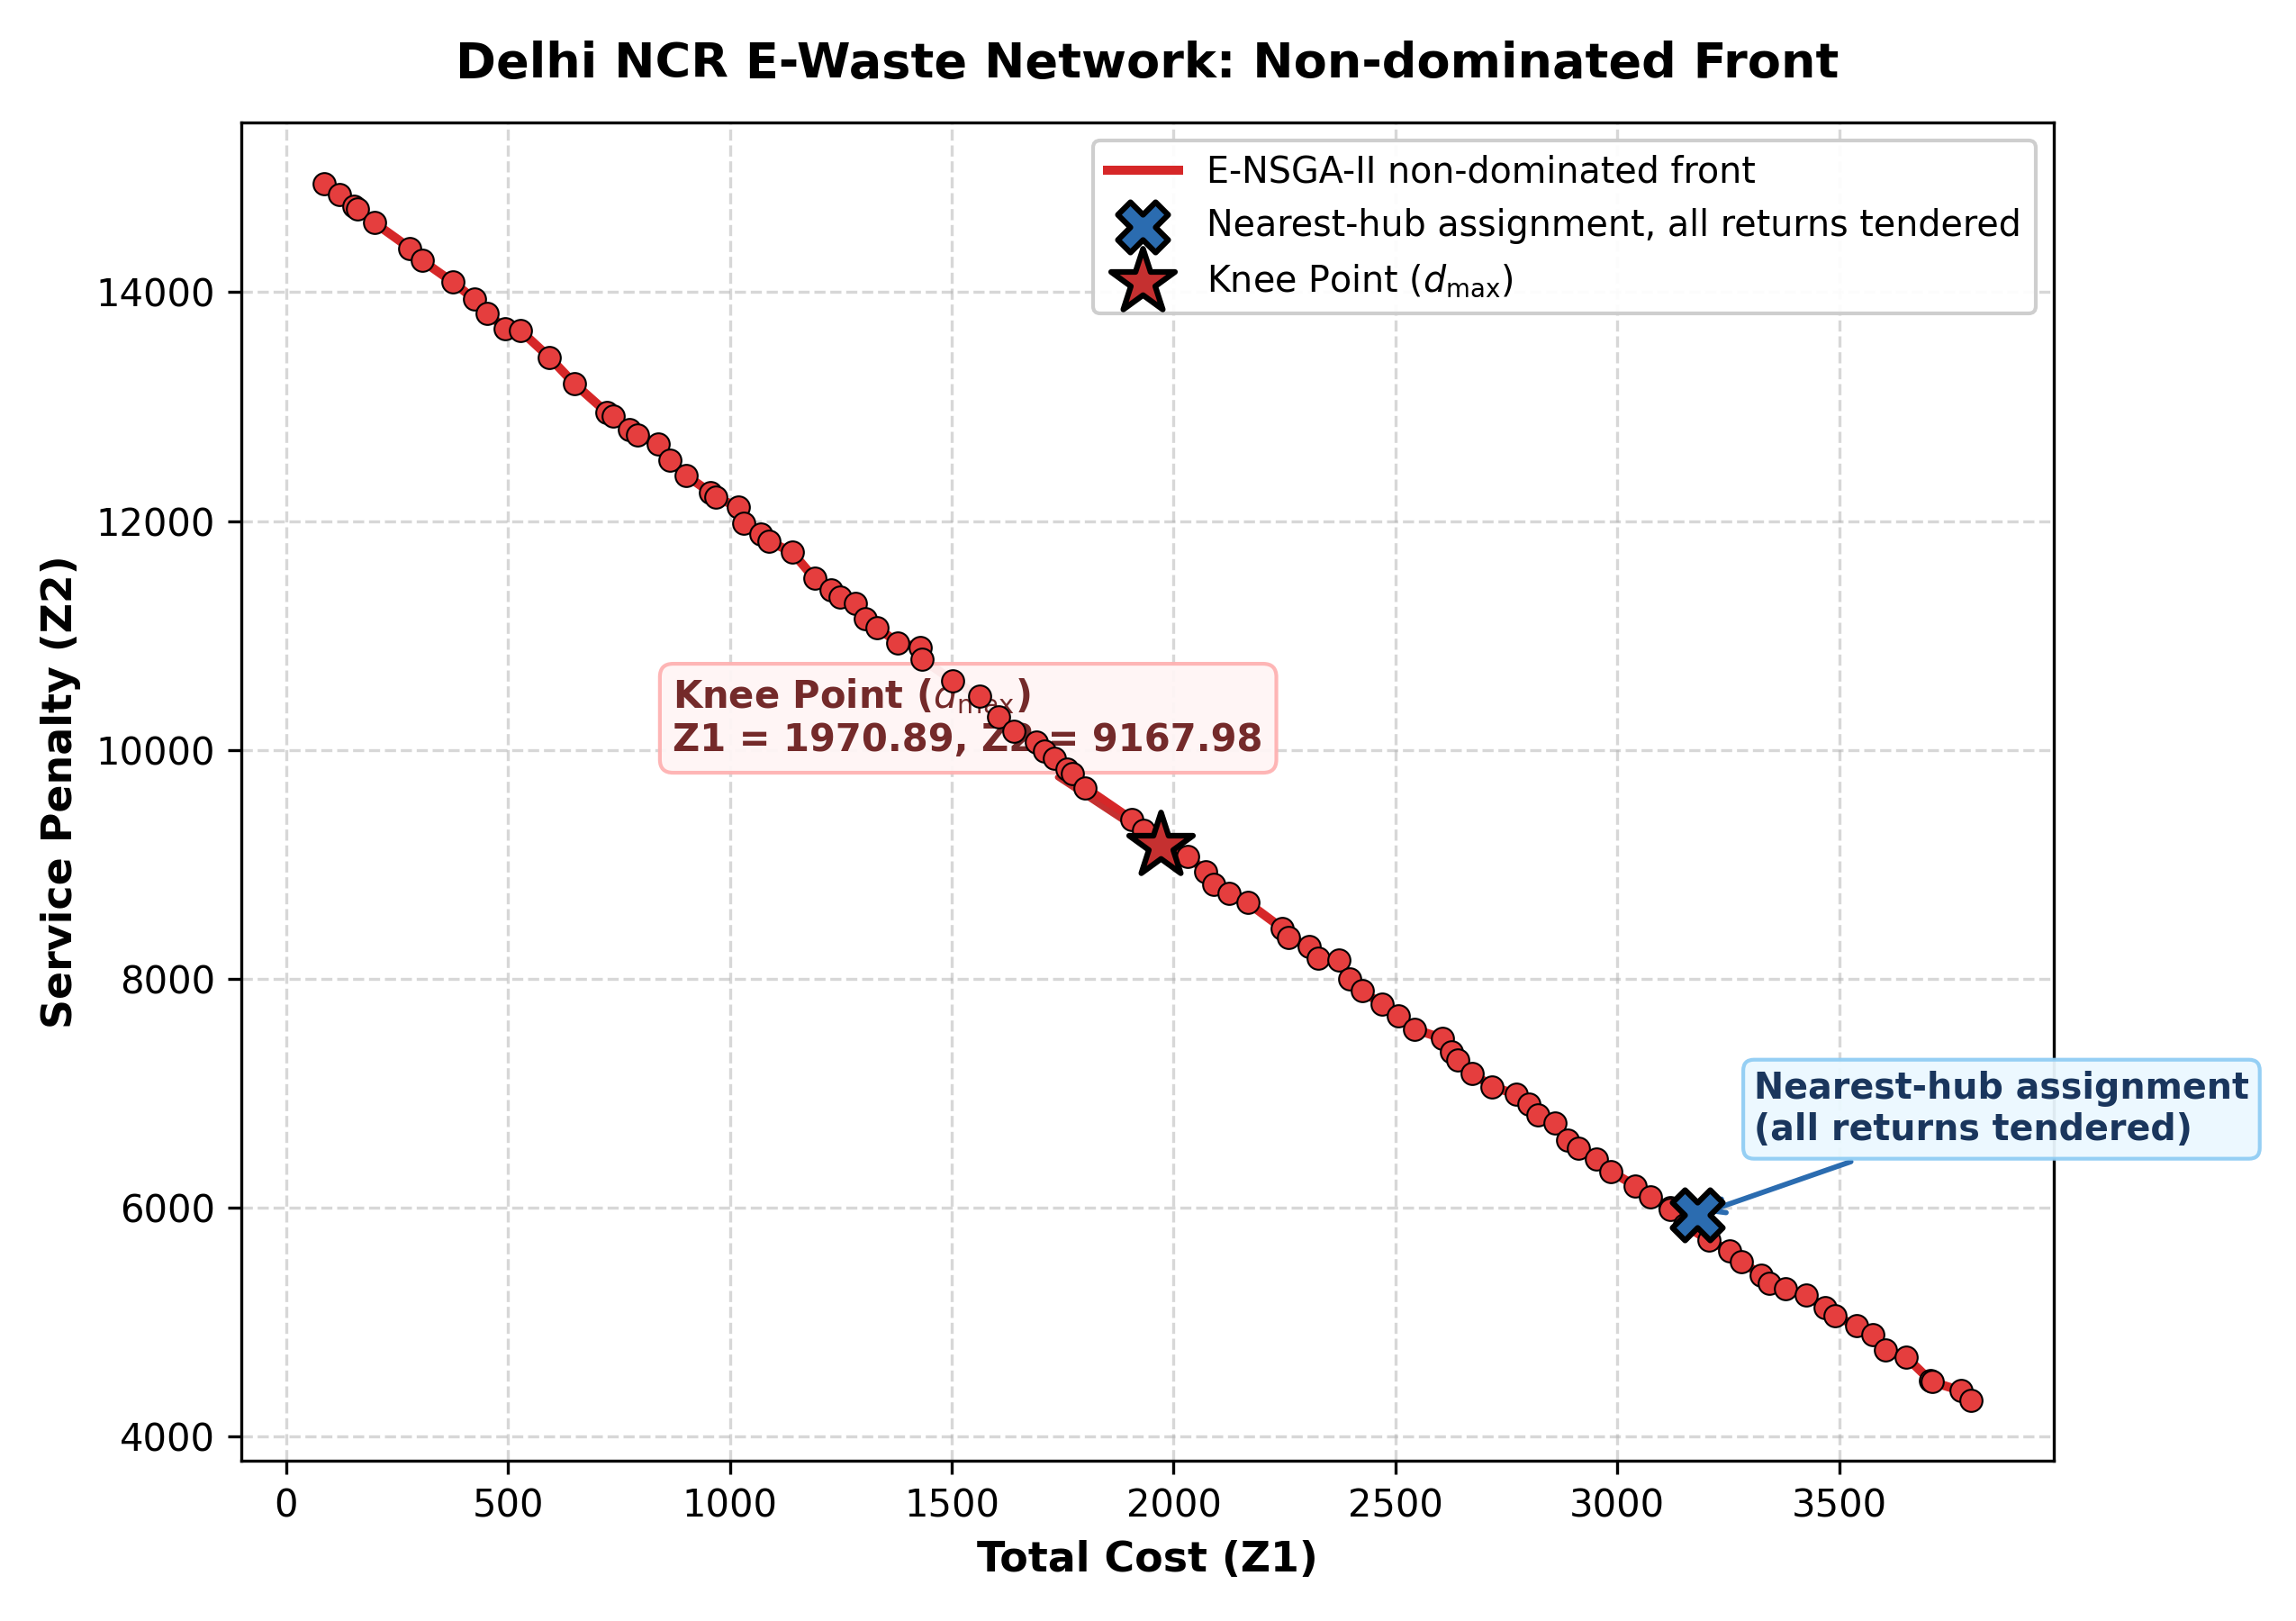
\includegraphics[width=\linewidth]{Delhi_Pareto_Front.png}
\end{minipage}\hfill
\begin{minipage}{0.49\textwidth}
\centering
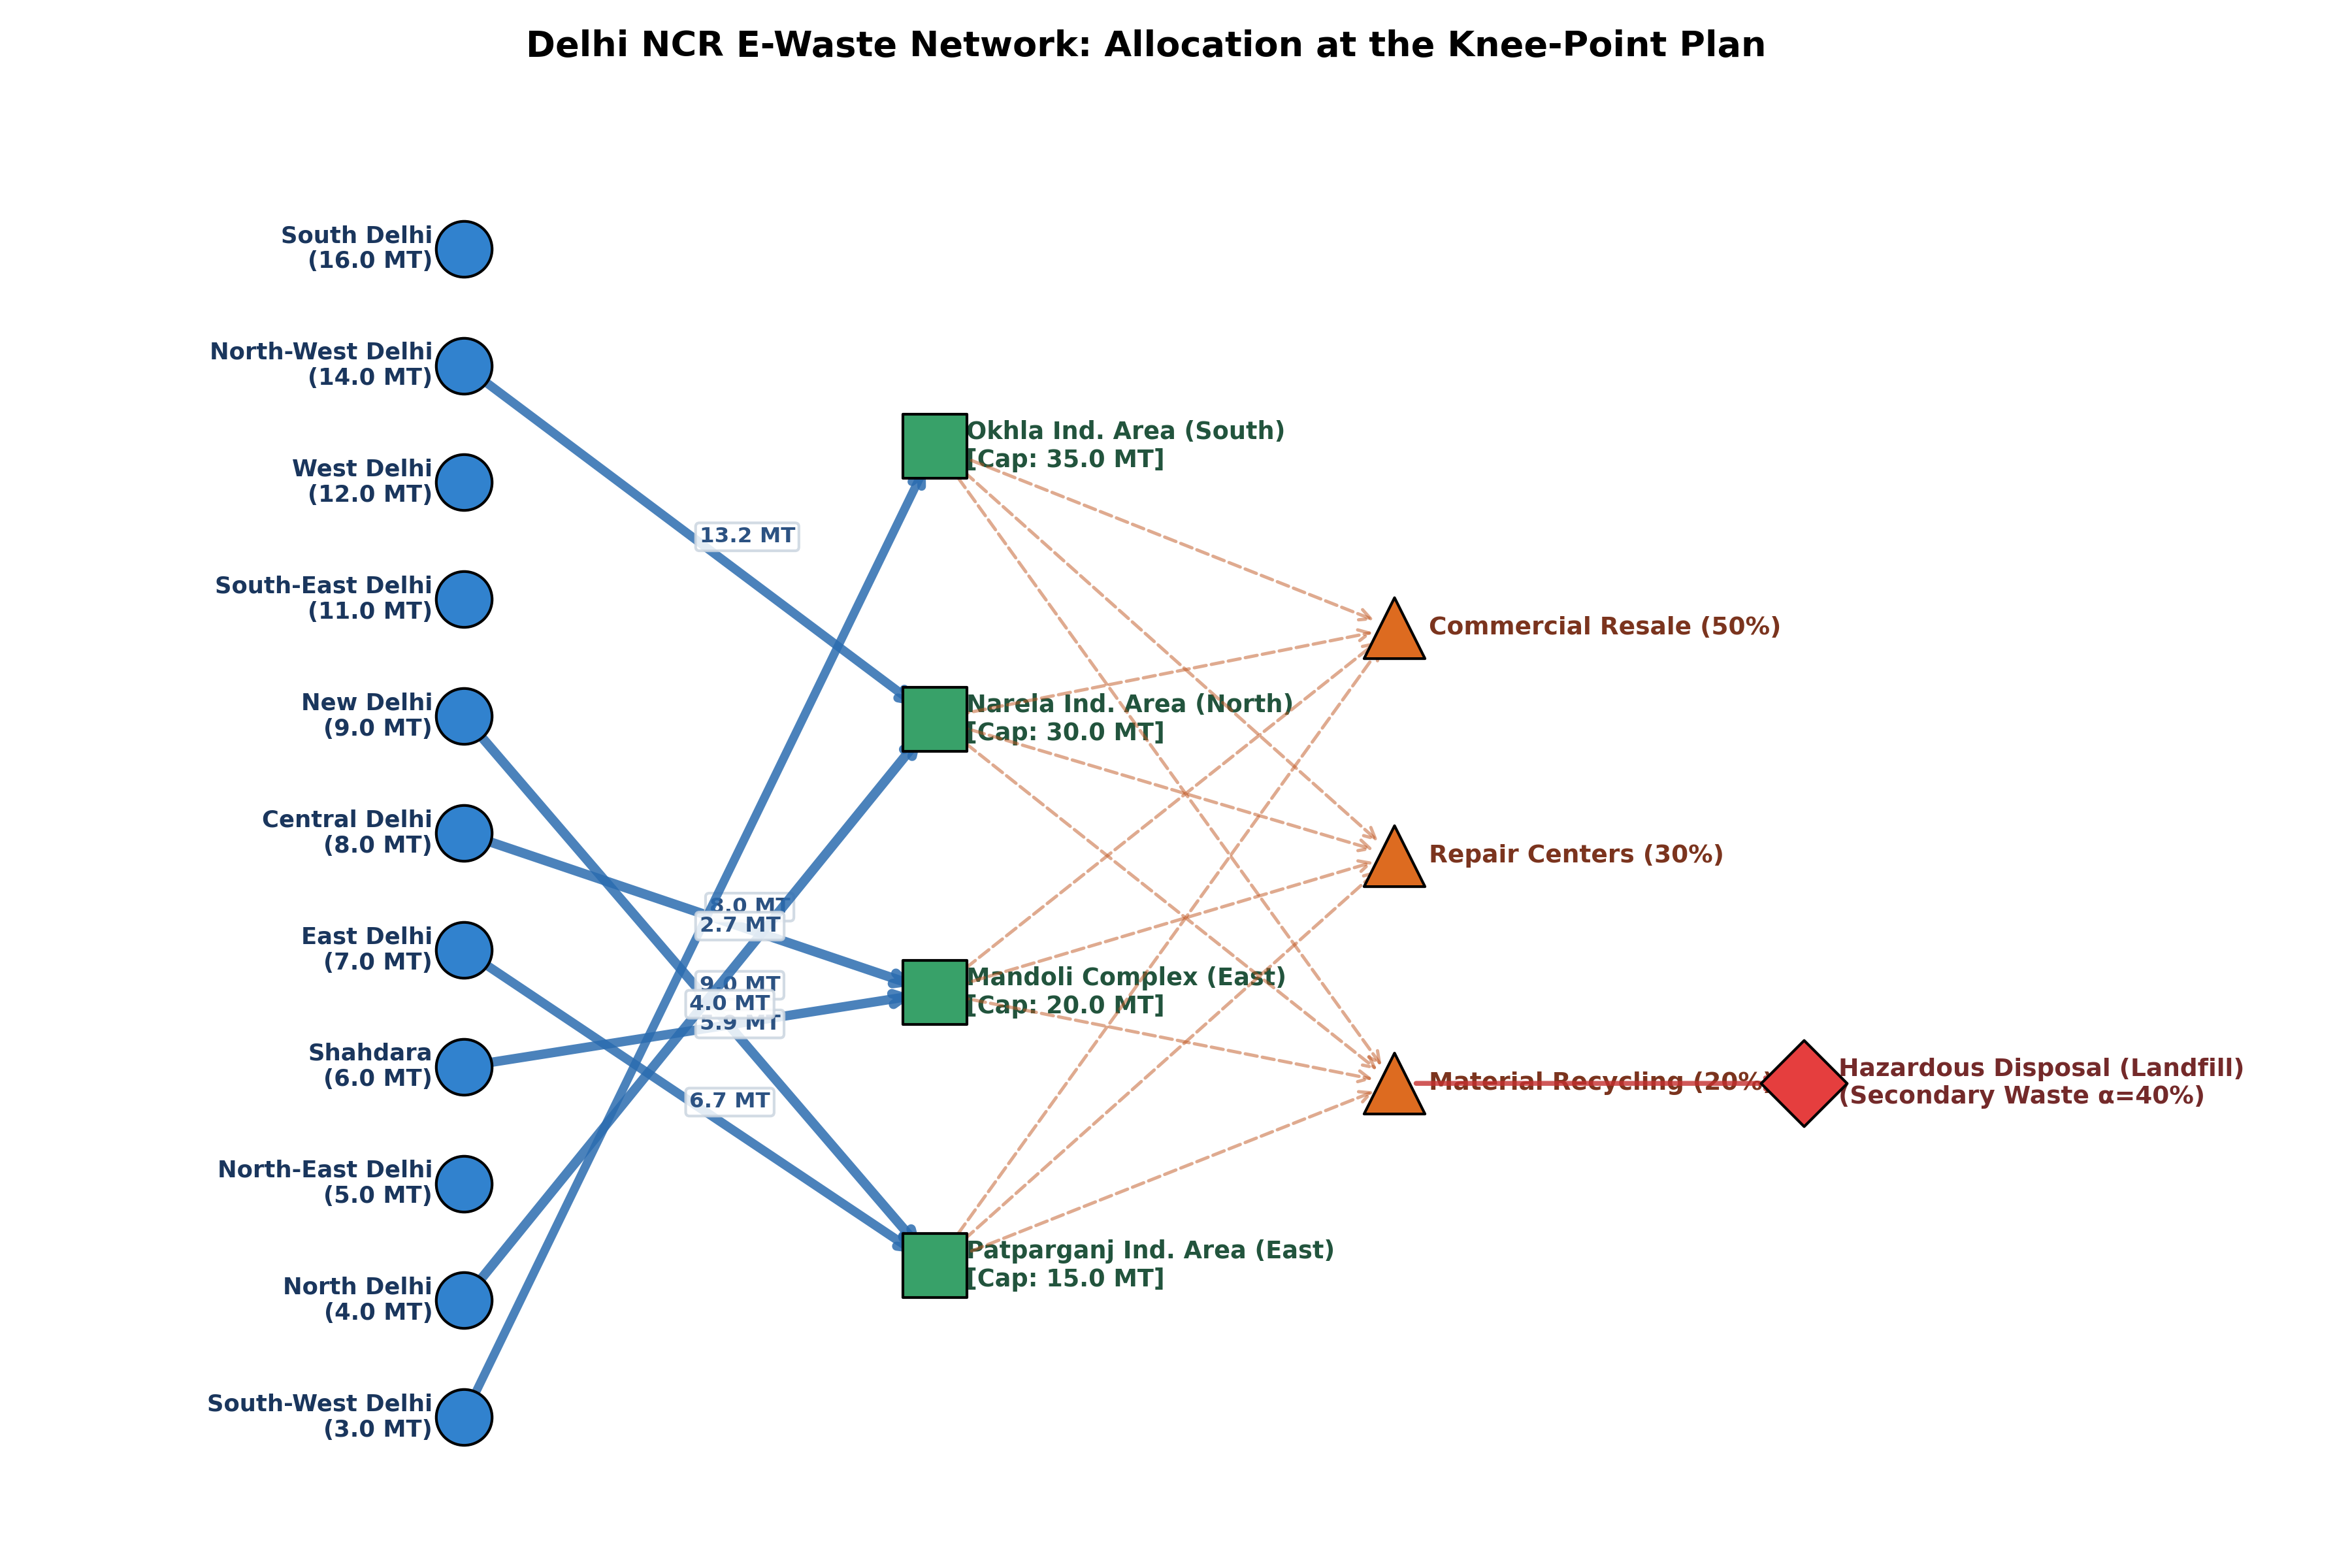
\includegraphics[width=\linewidth]{Delhi_Network_Flow.png}
\end{minipage}
\caption{Delhi NCR e-waste recovery network: non-dominated front (left) and allocation at the knee-point plan across the 11 administrative districts and 4 industrial recycling hubs (right). The cross marks the plan that assigns every district to its nearest hub and tenders all returns.}
\label{fig:DelhiResults}
\end{figure}

\subsubsection{Case study B: Greater London (United Kingdom)}\label{sec:case-london}

Greater London provides a benchmark of a mature Western/European reverse logistics network, operating under high labor costs, strict emission standards (the Ultra Low Emission Zone, ULEZ), and stringent Extended Producer Responsibility (EPR) mandates. The network operates under the UK Waste Electrical and Electronic Equipment (WEEE) Regulations, with municipal collection data published openly on the London Datastore and treatment facilities licensed as Approved Authorised Treatment Facilities (AATFs) by the UK Environment Agency (EA). The network consists of $|I| = 8$ representative borough groupings and $|J| = 3$ regional AATF treatment hubs:
\begin{enumerate}
    \item \textbf{Edmonton EcoPark} ($j=1$, North London).
    \item \textbf{Rainham \& Dagenham Resource Centre} ($j=2$, East London).
    \item \textbf{Beddington Farmlands Hub} ($j=3$, South London).
\end{enumerate}
The borough groupings are Westminster \& City, Barnet \& Enfield, Southwark \& Lambeth, Croydon \& Bromley, Camden \& Islington, Tower Hamlets \& Hackney, Kensington \& Chelsea, and Greenwich \& Lewisham, with a total mean regional return demand of 80.0 MT/scenario. The central financial boroughs, Westminster and the City of London, alone generate 18.0 MT/scenario of commercial IT equipment waste (more than double the next-largest source), while strict landfill-diversion targets demand high collection rates even as high urban transit costs require minimizing cross-Thames and orbital M25 transit miles.

Figure~\ref{fig:LondonResults} presents the non-dominated front and the allocation at the knee point. The mean total capacity of the three hubs is 89.9 MT/scenario. The front runs from the plan that collects nothing ($Z_1 = 0$, $Z_2 = 1.28\times10^{4}$) to $Z_1 = 3536$, $Z_2 = 9.6\times10^{2}$, and it is again close to a straight line. The knee-point plan has $Z_1 = 998.49$ and $Z_2 = 9.32\times10^{3}$ and collects 28.5\% of the returned volume on average (between 26.3\% and 31.3\% across the scenarios). It serves Southwark \& Lambeth, Kensington \& Chelsea and Greenwich \& Lewisham and collects almost nothing from the other five borough groupings, including Westminster \& City, the largest source. Beddington works at 72\% of its mean capacity, Rainham \& Dagenham at 13\% and Edmonton at 2\%. As a plan for a network under landfill-diversion targets this would not be acceptable, and a provider would choose a point much further towards the service end of the front.

\begin{figure}[htbp]
\centering
\begin{minipage}{0.49\textwidth}
\centering
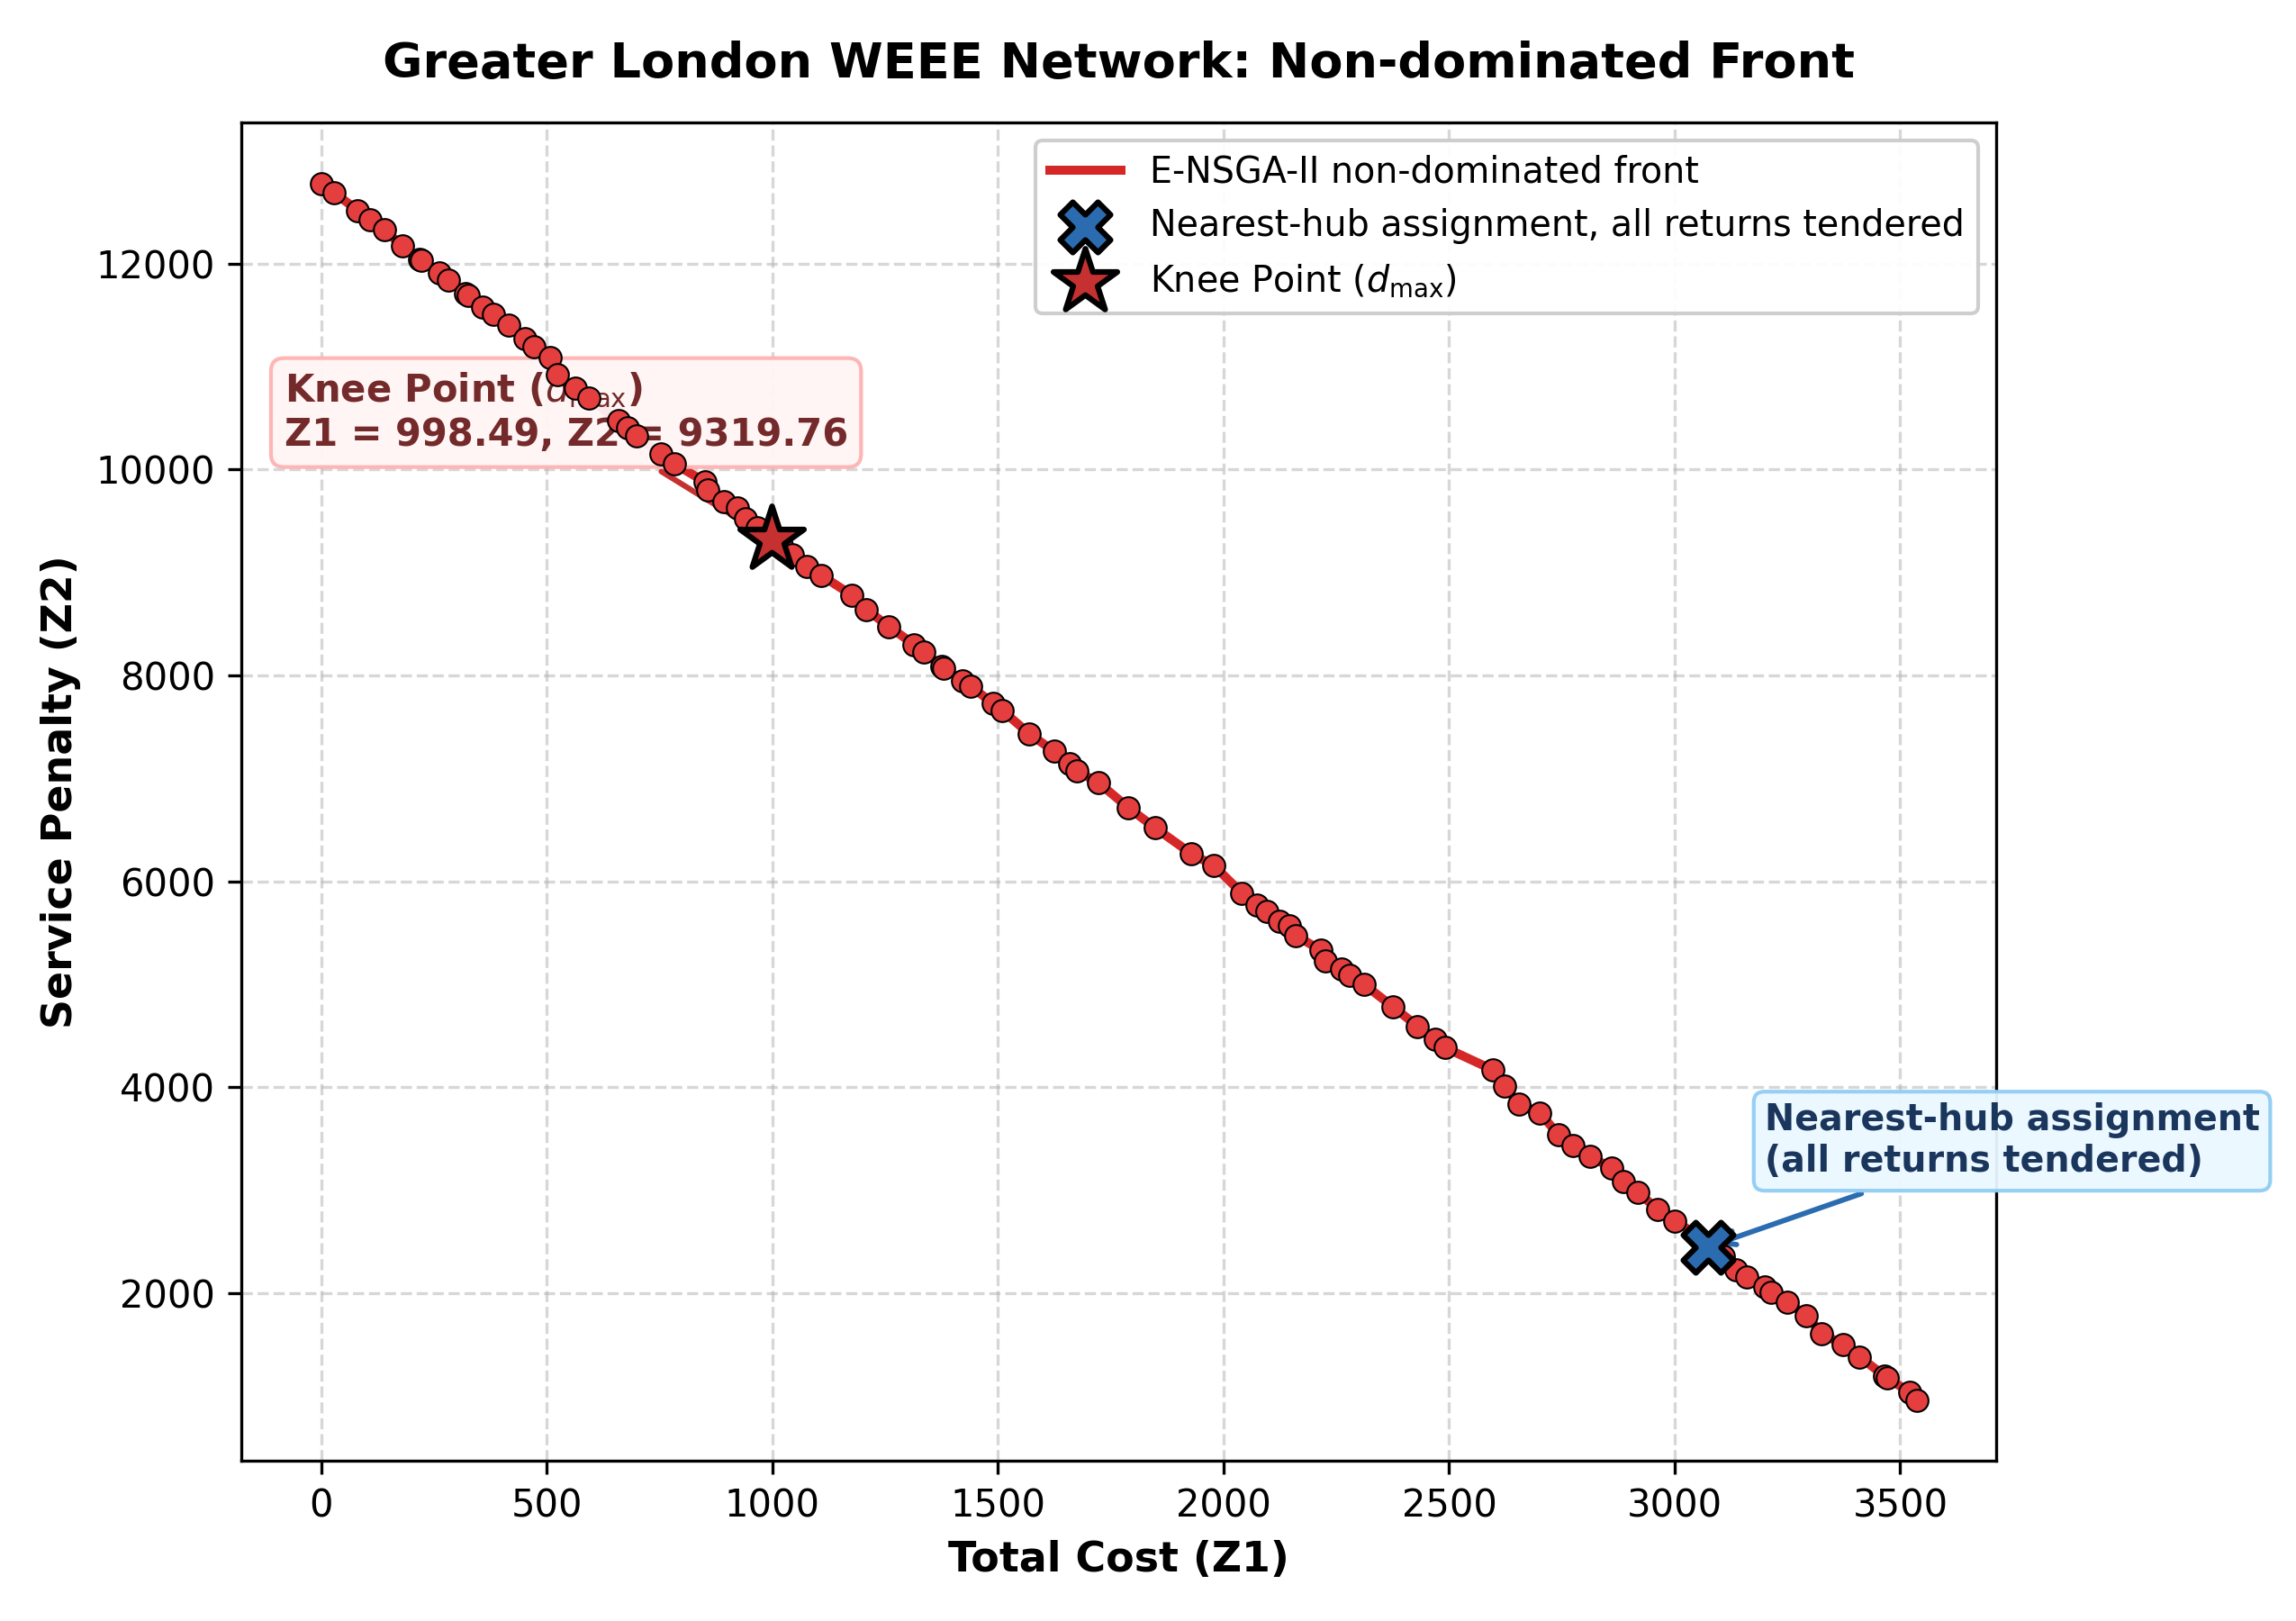
\includegraphics[width=\linewidth]{London_Pareto_Front.png}
\end{minipage}\hfill
\begin{minipage}{0.49\textwidth}
\centering
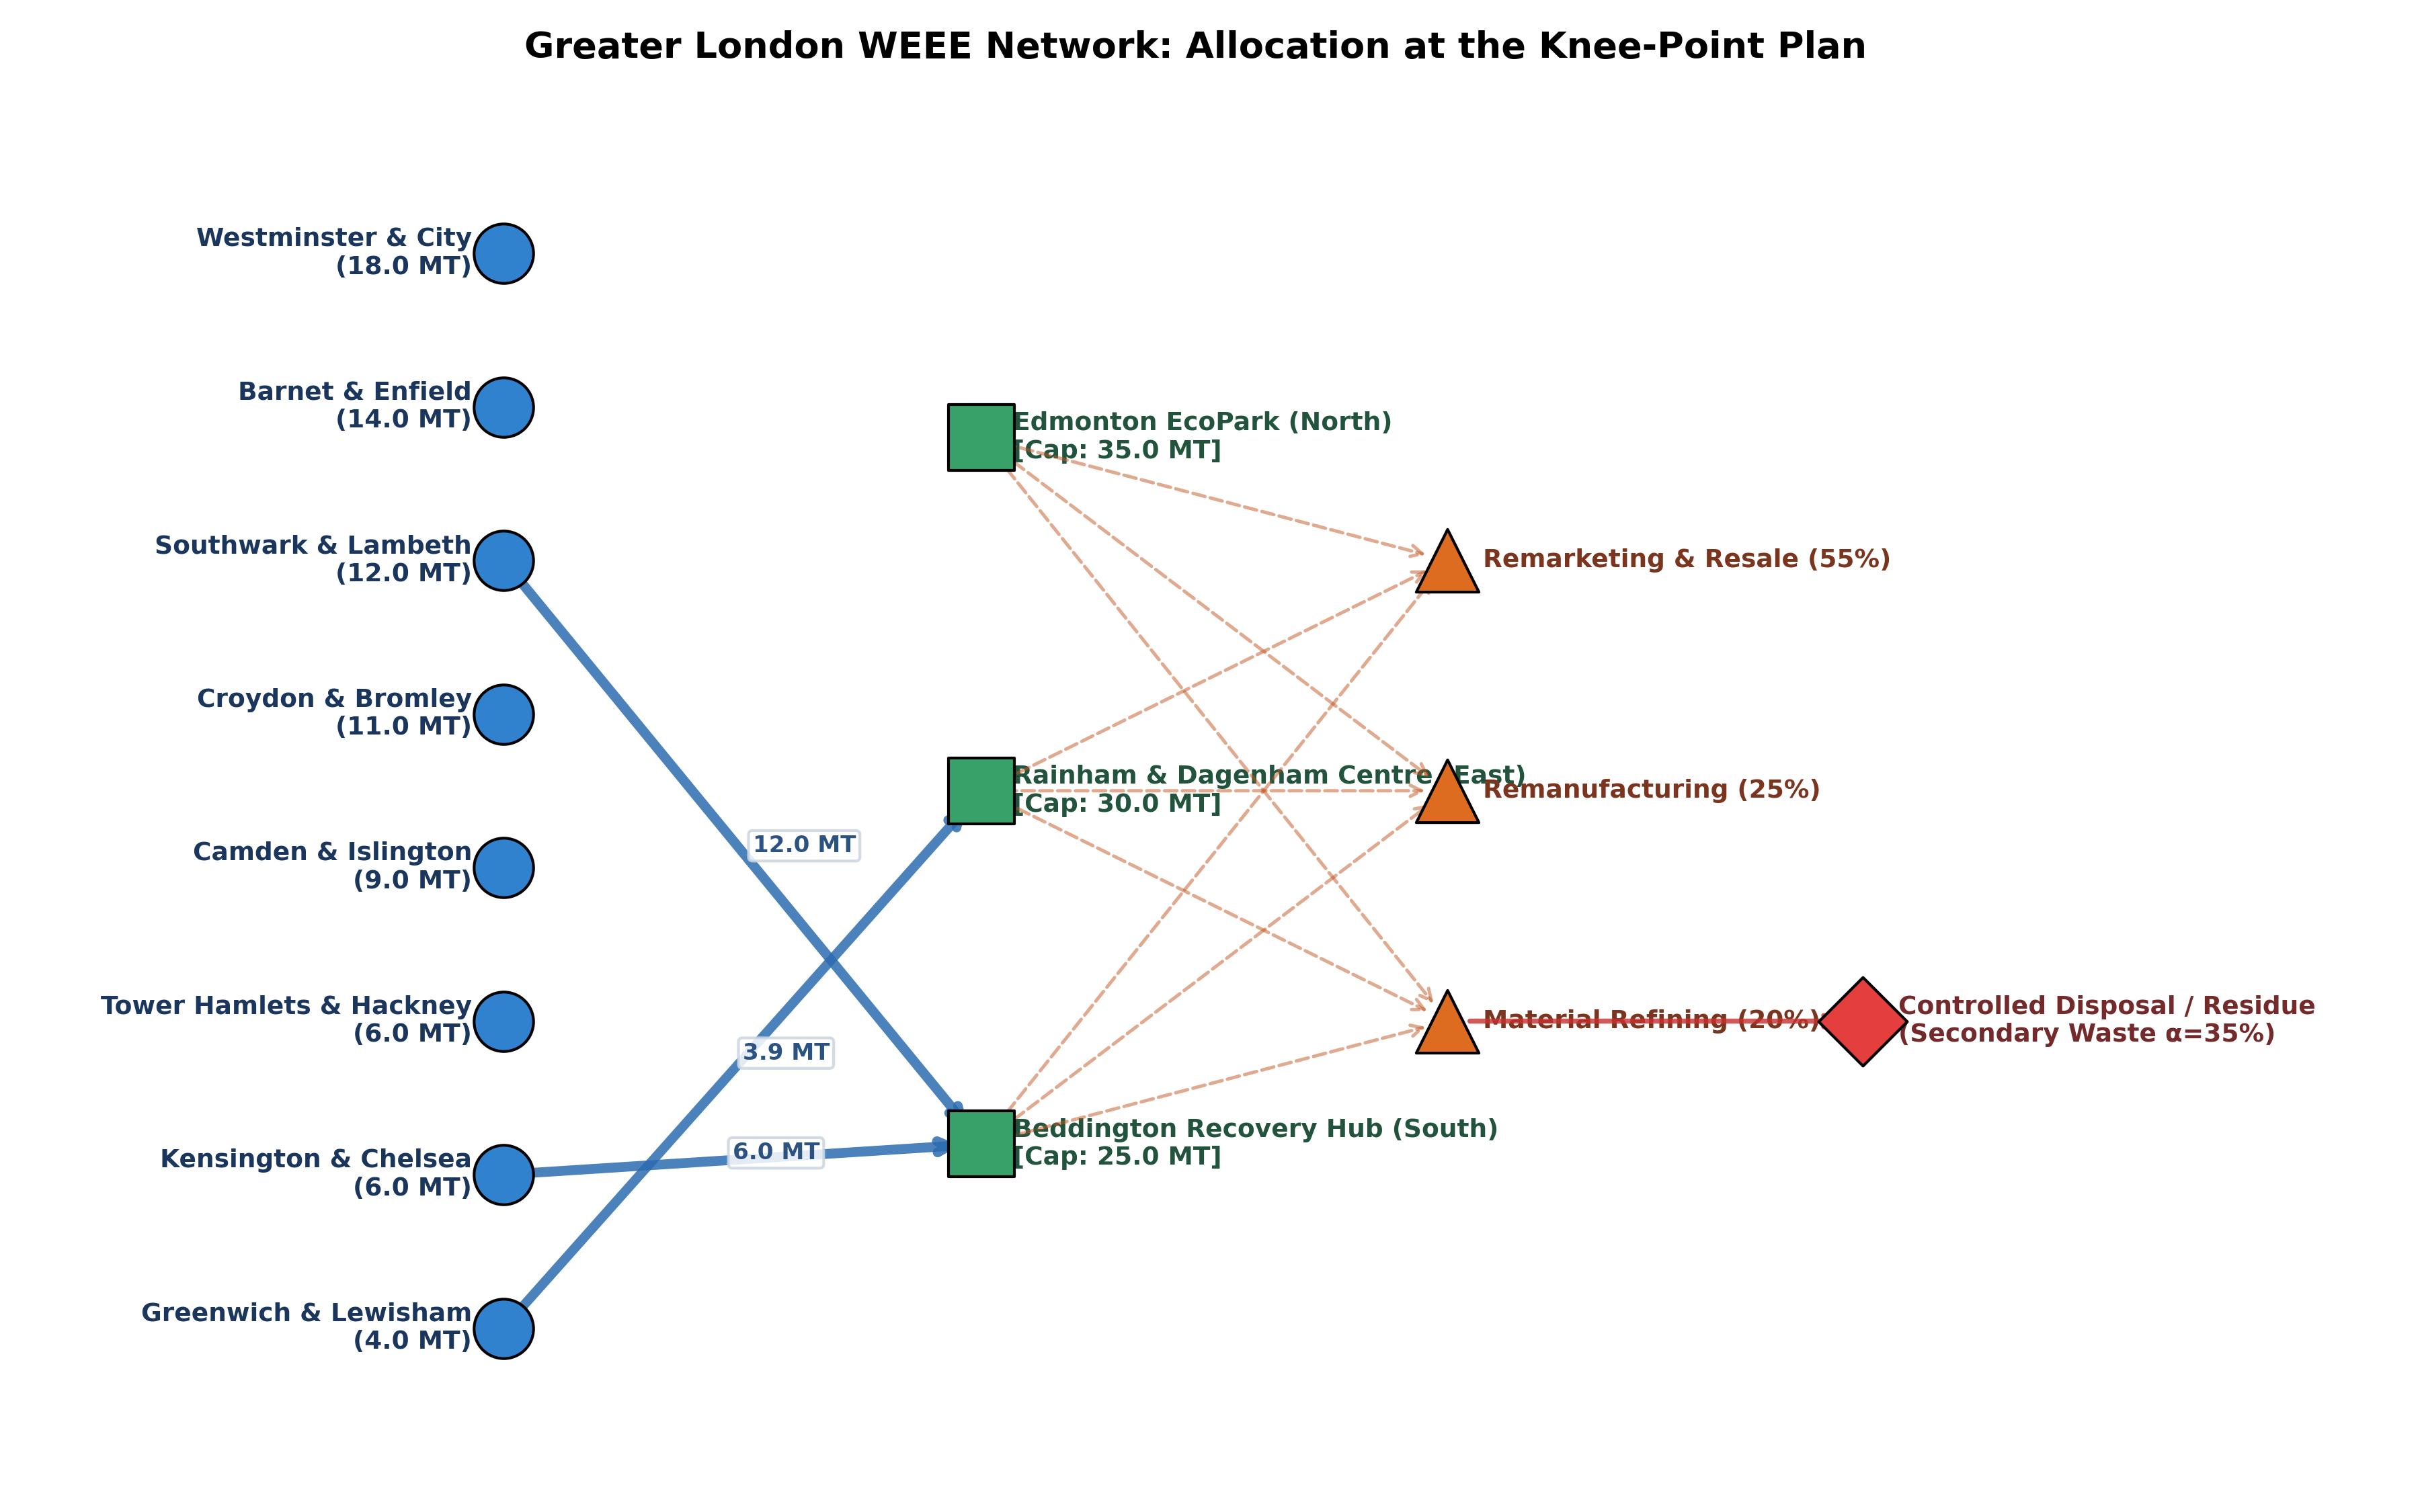
\includegraphics[width=\linewidth]{London_Network_Flow.png}
\end{minipage}
\caption{Greater London e-waste recovery network: non-dominated front (left) and allocation at the knee-point plan across the 8 borough groupings and 3 regional AATF treatment hubs (right). The cross marks the plan that assigns every borough grouping to its nearest hub and tenders all returns.}
\label{fig:LondonResults}
\end{figure}

\subsubsection{Cross-city comparative findings}\label{sec:cross-city-findings}

Table~\ref{tab:CrossCity} summarizes the two case studies. Three observations hold in both networks.

\begin{table}[htbp]
\centering
\small
\caption{Cross-city summary of network scale and of the E-NSGA-II knee-point plan.}
\label{tab:CrossCity}
\begin{tabular}{@{}lccccccc@{}}
\toprule
Case study & $|I|$ & $|J|$ & Mean returns & Mean capacity & Knee $Z_1$ & Knee $Z_2$ & Collection rate \\
 & & & (MT/scenario) & (MT/scenario) & & & (\%) \\
\midrule
Delhi NCR & 11 & 4 & 95.2 & 99.7 & 1970.89 & 9167.98 & 51.8 \\
Greater London & 8 & 3 & 79.9 & 89.9 & 998.49 & 9319.76 & 28.5 \\
\bottomrule
\end{tabular}
\end{table}

\textbf{The knee point is a low-collection plan.} In both networks the trade-off between cost and penalty is almost linear, so the point of maximum distance from the chord is not a pronounced knee, and it falls where roughly half (Delhi) or less than a third (London) of the returns are collected. The plan concentrates collection on a subset of zones and leaves the others, including the largest one in each city, uncollected. These plans are reported as the output of the procedure of Section~4.4 and not as recommendations.

\textbf{Cost differences between plans reflect how much is collected.} An earlier version of this section compared the knee-point plan with a plan that assigns each zone to its nearest hub and tenders all returns, described that plan as current industry practice, and reported the difference in $Z_1$ as a saving of 38.0\% and 67.5\%. We have withdrawn those figures. We have no source showing that providers operate in this way, and the comparison was not made at equal service. The nearest-hub plan collects 83.3\% of the returns in Delhi and 87.2\% in London, against 51.8\% and 28.5\% at the knee point, and its penalty $Z_2$ is correspondingly lower ($5.94\times10^{3}$ and $2.45\times10^{3}$). The difference in $Z_1$ was the cost of the volume that the knee-point plan does not collect. When the comparison is made at the same service level it disappears: the cheapest point of the E-NSGA-II front whose penalty is no higher than that of the nearest-hub plan costs 3151.61 against 3180.93 in Delhi, a difference below 1\%, and in London no point of the front dominates the nearest-hub plan at all (the cheapest front point with no higher penalty costs 3107.35 against 3074.20). In these two networks the nearest-hub assignment with full tendering is, in effect, a point at the high-service end of the front.

\textbf{What the case studies show.} The framework runs on networks built around named facilities and districts under two different regulatory settings and returns a complete trade-off curve from which a provider can pick a collection level. The case studies do not show that it improves on what providers do today. Like the other results of Section~5, the fronts were obtained with the scenario-independent collection rule of Section~\ref{sec:representation}, so they are subject to the restriction quantified in Section~\ref{validation-against-exact-solutions}.
\section{Managerial Implications}
The results carry four practical messages for a 3PL provider planning a returns network under a service contract. The collection level, not the choice of hub, drives the cost of a plan. In both case networks the cost and penalty of a plan move almost one for one with the volume collected, and a plan that sends every zone to its nearest hub and tenders all returns lies on or very close to the trade-off curve at its high-service end. Reassigning zones away from their nearest hub pays only where that hub's capacity binds. Two plans should therefore be compared on cost only at the same service level, since a cheaper plan is usually one that collects less. The first question for the provider is how much of the returned volume the contract obliges it to collect, and the assignment of zones to collection centres follows from that.

The knee point is a possible default operating plan on the benchmark instances, but it needs checking against the collection obligation. In the two case networks the knee point falls at collection rates of 52\% and 29\%, which a contract with collection targets would not allow. In instance 8, moving from the cost-orientated weighting $(0.7,0.3)$ to the service-orientated weighting $(0.3,0.7)$ lifts the collection rate from 52.80\% to 65.47\% and cuts the late-delivery penalty from 189{,}246.83 to 165{,}985.39, but operating costs rise from 463{,}147.29 to 521{,}223.28, a premium of 12.5\%. The knee point coincides with the balanced weighting
and captures most of the service gain (60.71\% collection, 34{,}420 uncollected units) at roughly half that premium. Where no explicit client preference is stated, the knee point gives the provider a plan that is easy to justify to both the operations and the account-management side of the contract.

Only two contract parameters are worth negotiating hard. The sensitivity analysis shows that effective collection-centre capacity $\widetilde{Ca}_j$ and the uncollected-return penalty rate $\phi_1$ dominate: a $\pm 35\%$ swing in capacity moves total cost by about 81\%, while $\phi_1$ acts as a near-pure multiplier on the penalty
term, taking it from 8.13 to 16.42 million over the same range. Sorting fractions, the e-waste fraction and the late-delivery penalty rate shift the totals by less than 2\%. Negotiating effort, data collection, and staffing flexibility should therefore concentrate on capacity assurance and the uncollected-volume clause. Because the penalty enters the cost objective as well, a client or regulator that tightens $\phi_1$ raises the
provider's total logistics cost, not merely its penalty exposure.

Planning does not require heavy computational infrastructure. Plans selected on 50 in-sample scenarios shift by at most 3.1\% on cost and 0.3\% on service when re-evaluated on 500 unseen realizations, and the ranking of plans is unchanged under Normal and Lognormal return distributions. These figures concern the stability of a plan across scenario samples. They do not say how close the plan is to the best attainable one. On the three small instances where that can be checked, the plans produced with the fixed collection rule cost between 28\% and 135\% more than an exact plan with the same service level (Table~\ref{tab:TwoGaps}), and the gap closes when the collected quantities are allowed to adapt to each scenario. With solution times of 3--7 seconds on the benchmark instances, the provider can re-run the plan at every contract renewal, or whenever return volumes drift, without specialized solver infrastructure.

\section{Conclusion}

This paper has addressed the reverse logistics planning problem of a third-party logistics provider that commits to a service contract before knowing the return volumes, collection capacities, handling and storage costs, and repair turnaround times it will face. The problem was formulated as a bi-objective two-stage stochastic mixed-integer linear programm in which the first stage fixes the assignment of customer zones to collection
centres and the second stage determines the recourse flows across the collection, retailing, repair, recycling and disposal echelons, including the explicit return leg that carries repaired items back to the customers who sent them. The scope was deliberately restricted to the decisions a provider actually controls, and service performance was measured through the contractual penalties for uncollected returns and late deliveries
rather than through a distance or travel-time proxy.

An Enhanced NSGA-II was developed as an approximate solution method. It searches over the assignments and a scenario-independent collection rule, and it has three
problem-specific components: cost-structure-based heuristic initialisation, a feasibility-preserving repair operator, and adaptive mutation triggered by the loss of diversity along the Pareto front. Benchmarked against MOEA/D-DE, SMS-EMOA and SPEA2 under a common evaluation budget, E-NSGA-II attained the best mean hypervolume on ten of twelve instances and the best $\text{IGD}^+$ and spread on all twelve, with the Friedman test
rejecting equal performance on every indicator ($p < 0.001$), and it did so at the lowest computational cost. The ablation study confirmed that both enhancements contribute, that they matter more for diversity than for convergence, and that their effects interact. The objective values of the selected plans moved by at most 3.1\% on cost and 0.3\% on service between the in-sample and the out-of-sample scenarios, the plans held their ranking under alternative distributional assumptions, and the method scaled to networks of 50--100 customer zones. The out-of-sample figures measure how well a plan generalizes across scenario samples and are distinct from its distance to the exact front, which is reported separately below. The framework was also applied to two networks built around the Delhi NCR and Greater London e-waste recovery systems. Their knee-point plans collect 51.8\% and 28.5\% of the returned volume, and the trade-off between cost and penalty in both networks is close to linear. No claim of savings over current practice is made, since we have no documented comparator.

Several limitations bound these conclusions and point to further work. The formulation is single-period and single-product, so it cannot represent seasonal return surges, inventory carried between periods, or return streams whose recovery options differ by product family; extending it to a multi-period, multi-product setting is the most immediate generalization. The recourse structure is risk-neutral, optimizing expected cost and
expected penalty; because a provider's contractual exposure is driven by tail realizations, a mean-risk or CVaR variant would be a more faithful representation of how penalty clauses are experienced. Uncertainty is represented through sample average approximation on a finite scenario set, and although 50 scenarios proved sufficient here, no distributional-ambiguity guarantee is offered; distributionally robust counterparts are
a natural next step. The solution method does not search the full recourse space of the model. The fraction of returns that the provider attempts to collect in each zone is fixed across scenarios, capacity shortfalls are shared proportionally, and the repair channel is routed by cost alone, so the reported fronts are feasible for the two-stage model but belong to a restricted class of recourse policies. On instances 1--3, where a dense exact reference was computed, E-NSGA-II with this rule recovered 84.6\%, 88.5\% and 62.6\% of the exact hypervolume, which is not a close approximation, and its knee-point plans cost between 28\% and 135\% more than exact plans with the same service level even though their out-of-sample gap was about 1\%. When the recourse was instead solved inside the decoder, which reduces to a continuous knapsack problem at each collection center because the downstream facilities are uncapacitated, the same algorithm recovered more than 99\% on all three instances at no higher run time. The loss is therefore due to the restriction and not to the search. On instances 4--8, 10, 12 and 15, against reference fronts computed with an open-source solver under a budget of 300 seconds per subproblem, the rule recovered between 85\% and 28\% of the reference hypervolume, falling as the instance grows, and the recourse variant stayed at the level of the reference. The exact method proved optimality at every grid point up to instance~5 and returned fronts with gaps of about 4\% at most on the largest instance in under two hours, so the argument for the evolutionary method on this benchmark is its run time of seconds and not the intractability of exact solution, and on the two smallest instances the exact method is as fast or faster and should be preferred. Beyond that, the method is a metaheuristic and provides no optimality gap on instances of realistic size, so pairing it with an L-shaped or Benders decomposition to certify the quality of the front would strengthen the evidence. Finally, the model takes the penalty rates as exogenous, whereas the sensitivity analysis shows that $\phi_1$ is the single most influential contractual parameter; treating the contract itself as a decision, in a bilevel or Stackelberg setting between client and provider, would close the loop between network planning and contract design.
\subsubsection*{Data Availability Statement}
\footnotesize All benchmark instance parameters and configurations are fully reported within the manuscript (Tables 6–8 and Table 21). Empirical case study data for Delhi NCR and Greater London were derived from publicly accessible regulatory sources (DPCC, CPCB, UK EA, and London Datastore) cited in the text. The curated datasets supporting the findings of this study are available from the corresponding author upon reasonable request.
\bibliographystyle{plainnat}
\bibliography{Ref1}
\end{document}